\RequirePackage[l2tabu,orthodox]{nag}

% TODO: decide if one-sided/two-sided
%\documentclass[headsepline,footsepline,footinclude=false,fontsize=11pt,paper=a4,listof=totoc,bibliography=totoc,BCOR=12mm,DIV=12]{scrbook} % two-sided
\documentclass[headsepline,footsepline,footinclude=false,oneside,fontsize=11pt,paper=a4,listof=totoc,bibliography=totoc]{scrbook} % one-sided

\PassOptionsToPackage{table,svgnames,dvipsnames}{xcolor}

\usepackage[utf8]{inputenc}
\usepackage[T1]{fontenc}
\usepackage[sc]{mathpazo}
\usepackage[american]{babel}
\usepackage[autostyle]{csquotes}
\usepackage[%
  backend=biber,
  url=false,
  style=alphabetic,
  maxnames=4,
  minnames=3,
  maxbibnames=99,
  firstinits,
  uniquename=init]{biblatex} % TODO: adapt bibliography style
\usepackage{graphicx}
\usepackage{scrhack} % necessary for listings package
\usepackage{listings}
\usepackage{lstautogobble}
\usepackage{tikz}
\usepackage{pgfplots}
\usepackage{pgfplotstable}
\usepackage{booktabs}
\usepackage[final]{microtype}
\usepackage{caption}
\usepackage[hidelinks]{hyperref} % hidelinks removes colored boxes around references and links
\usepackage[toc,nonumberlist,acronym]{glossaries} % TODO: remove if glossary not needed
\usepackage{textcomp}
\usepackage[boxruled,linesnumbered,lined,commentsnumbered,longend,nofillcomment,noresetcount]{algorithm2e}
\usepackage{amsmath}
\usepackage{mathtools}
\usepackage[all]{hypcap}

\bibliography{bibliography/literature}

\setkomafont{disposition}{\normalfont\bfseries} % use serif font for headings
\linespread{1.05} % adjust line spread for mathpazo font

% Settings for glossaries TODO: remove the following block if glossary not needed
\renewcommand{\glsnamefont}[1]{\normalfont\bfseries #1} % use serif font for glossary entry titles
\makeglossaries{}

% Settings for pgfplots
\pgfplotsset{compat=1.9} % TODO: adjust to your installed version
\pgfplotsset{
  % For available color names, see http://www.latextemplates.com/svgnames-colors
  cycle list={CornflowerBlue\\Dandelion\\ForestGreen\\BrickRed\\},
}

% Settings for lstlistings
\lstset{%
  basicstyle=\ttfamily,
  columns=fullflexible,
  autogobble,
  keywordstyle=\bfseries\color{MediumBlue},
  stringstyle=\color{DarkGreen}
}

% Basic information for cover & title page
\newcommand*{\getUniversity}{Technische Universität München}
\newcommand*{\getFaculty}{Department of Informatics}
\newcommand*{\getTitle}{Job Scheduling for Adaptive Applications in Future HPC Systems}
\newcommand*{\getTitleGer}{Job Scheduling für Adaptive Anwendungen auf Zukünftigen HPC Systemen}
\newcommand*{\getAuthor}{Nishanth Nagendra}
\newcommand*{\getDoctype}{Master's Thesis in Informatics}
\newcommand*{\getSupervisor}{Prof. Dr. Michael Gerndt}
\newcommand*{\getAdvisor}{M.Sc. Isaias Alberto Compres Urena}
\newcommand*{\getSubmissionDate}{May 15, 2015}
\newcommand*{\getSubmissionLocation}{Munich}

% TODO: add custom commands etc.


% TODO: remove if glossary not needed
\newglossaryentry{computer}
{
  name=computer,
  description={is a machine that\ldots}
}

\newacronym{tum}{TUM}{Technische Universität München}


\begin{document}

\begin{titlepage}
  % HACK for two-sided documents: ignore binding correction for cover page.
  % Adapted from Markus Kohm's KOMA-Script titlepage=firstiscover handling.
  % See http://mirrors.ctan.org/macros/latex/contrib/koma-script/scrkernel-title.dtx,
  % \maketitle macro.
  \oddsidemargin=\evensidemargin\relax
  \textwidth=\dimexpr\paperwidth-2\evensidemargin-2in\relax
  \hsize=\textwidth\relax

  \centering

  \includegraphics[width=40mm]{logos/tum}

  \vspace{5mm}
  {\huge\MakeUppercase{\getFaculty{}}}\\

  \vspace{5mm}
  {\large\MakeUppercase{\getUniversity{}}}\\

  \vspace{20mm}
  {\Large \getDoctype{}}

  \vspace{15mm}
  {\huge\bfseries \getTitle{}}

  \vspace{15mm}
  {\LARGE \getAuthor{}}

  \vspace{20mm}
  \includegraphics[width=20mm]{logos/faculty}
\end{titlepage}


\frontmatter{}

\begin{titlepage}
  \centering

  \includegraphics[width=40mm]{logos/tum}

  \vspace{5mm}
  {\huge\MakeUppercase{\getFaculty{}}}\\

  \vspace{5mm}
  {\large\MakeUppercase{\getUniversity{}}}\\

  \vspace{20mm}
  {\Large \getDoctype{}}

  \vspace{15mm}
  {\huge\bfseries \getTitle{}}

  \vspace{10mm}
  {\huge\bfseries \getTitleGer{}}

  \vspace{15mm}
  \begin{tabular}{l l}
    Author: & \getAuthor{} \\
    Supervisor: & \getSupervisor{} \\
    Advisor: & \getAdvisor{} \\
    Submission Date: & \getSubmissionDate{} \\
  \end{tabular}

  \vspace{20mm}
  \includegraphics[width=20mm]{logos/faculty}
\end{titlepage}

\thispagestyle{empty}
\vspace*{0.8\textheight}
\noindent
I confirm that this \MakeLowercase{\getDoctype{}} is my own work and I have documented all sources and material used.

\vspace{15mm}
\noindent
\getSubmissionLocation{}, \getSubmissionDate{} \hspace{5cm} \getAuthor{}

\cleardoublepage{}

\addcontentsline{toc}{chapter}{Acknowledgments}
\thispagestyle{empty}

\vspace*{2cm}

\begin{center}
{\usekomafont{section} Acknowledgments}
\end{center}

\vspace{1cm}

%TODO: Acknowledgments
<TBA>
\cleardoublepage{}

\chapter{\abstractname}
Invasive Computing is a novel paradigm for the design and resource-aware programming of future parallel computing systems. It enables the programmer to write resource aware programs and the goal is to optimize the program for the available resources. Traditionally, parallel applications implemented using MPI are submitted with a fixed number of MPI processes to execute on a HPC(High Performance Computing) system. This results in a fixed allocation of resources for the job. Modern techniques in scientific computing such as AMR(Adaptive Mesh Refinement) result in applications exhibiting complex behaviors where their resource requirements change during execution. Invasive MPI is an ongoing research effort to provide MPI extensions for the development of Invasive MPI applications that will result in jobs which are resource-aware for the HPC systems and can utilize such AMR techniques. Unfortunately, using only static allocations result in these applications being forced to execute using their maximum resource requirements that may lead to inefficient resource utilization. In order to support such kind of parallel applications at HPC centers, there is an urgent need to investigate and implement extensions to existing resource management systems or develop a new system. This thesis has extended the previous work during which a protocol was developed for the intgeration of invasive resource management into existing batch systems. In this work, we have explored the idea of separating the concerns of batch and runtime scheduling into two different software layers / components in contrasts to existing systems where both are merged together. Specifically, This thesis has investigated and implemented a job scheduling algorithm in accordance with the new protocol developed earlier for supporting such an invasive resource management. An early prototype that can simulate the negotiation between batch and runtime scheduler using their respective scheduling algorithms for a HPC workload comprising different job types has been accomplished.\par

%TODO: Abstract



\microtypesetup{protrusion=false}
\tableofcontents{}
\microtypesetup{protrusion=true}
\listoffigures{}
\listoftables{}

\mainmatter{}

\chapter{Introduction}\label{chapter:introduction}
Over the last two decades, the landscape of Computer Architecture has changed radically from sequential to parallel . Due to the limiting factors of technology we have moved from single core processors to multi core processors having a network interconnecting them. Traditionally, the approach of designing algorithms has been sequential, but designing algorithms in parallel is gaining more importance now to better utilize the computing power available at our disposal. Another important trend that has changed the face of computing is an enormous increase in the capabilities of the networks that connect computers with regards to speed, reliability etc. These trends make it feasible to develop applications that use physically distributed resources as if they were part of the same computer. A typical application of this sort may utilize processors on multiple remote computers, access a selection of remote databases, perform rendering on one or more graphics computers, and provide real-time output and control on a workstation. Computing on networked computers ("Distributed Computing") is not just a subfield of parallel computing as the basic task of developing programs that can run on many computers at once is a parallel computing problem. In this respect, the previously distinct worlds of parallel and distributed computing are converging.\\ \par
\noindent
As technology advances, we have newer problems or applications that demand larger computing capabilities which push the limits of technology giving rise to newer advancements. The performance of a computer depends directly on the time required to perform a basic operation and the number of these basic operations that can be performed concurrently. A metric used to quantify the performance of a computer is FLOPS (floating point operations per second). The time to perform a basic operation is ultimately limited by the "clock cycle" of the processor, that is, the time required to perform the most primitive operation. The term \textbf{\textit{High Performance Computing (HPC)}} refers to the practice of aggregating computing power (multiple nodes with processing units interconnected by a network in a certain toplogy) or the use of parallel processing for running advanced application programs efficiently, reliably and quickly. The term applies especially to systems that function above a \textbf{\textit{teraflop}} or \textbf{\textit{$10^{12}$}} floating-point operations per second. The term HPC is occasionally used as a synonym for Supercomputer that works at more than a \textbf{\textit{petaflop}} or \textbf{\textit{$10^{15}$}} floating-point operations per second. The most common users of HPC systems are scientific researchers, engineers, government agencies including the military, and academic institutions. In general, HPC systems can refer to Clusters, Supercomputers, Grid Computing etc. and they are usually used for running complex applications.\\ \par
\noindent
A \textbf{\textit{Batch System}} is used to manage the resources in a HPC System. It is a middleware that comprises of two major components namely the \textbf{\textit{Resource Manager}} and \textbf{\textit{Scheduler}}. The role of a Resource Manager is to act like a glue for a parallel computer to execute parallel jobs. It should make a parallel computer as easy to use as a Personal Computer (PC). A programming model such as \textbf{\textit{Message Passing Interface (MPI)}} for programming on distributed memory systems would typically be used to manage communications within a parallel program by using the MPI library functions. A Resource Manager allocates resources within a HPC system, launches and otherwise manages Jobs. Some of the examples of widely used open source as well as commercial resource managers are \textbf{\textit{SLURM, TORQUE, OMEGA, IBM Platform LSF}} etc. Together with a scheduler it is termed as a Batch System. The role of a job scheduler is to manage queue(s) of work when there is more work than resources. It supports complex scheduling algorithms which are optimized for network topology, energy efficiency, fair share scheduling, advanced reservations, preemption, gang scheduling (time-slicing jobs) etc. It also supports resource limits (by queue, user, group, etc.). Many batch systems provide both resource management and job scheduling within a single product (e.g. LSF) while others use distinct products(e.g. Torque Resource Manager and Moab Job Scheduler). Some other examples of Job Scheduling Systems are \textbf{\textit{LoadLeveler, OAR, Maui, SLURM etc.}}\\ \par
\noindent
Existing Batch Systems usually support only static allocation of resources to Jobs/Applications before they start which means the resources once allocated are fixed for the lifetime of the application. The complexity of applications have been growing, However, especially when we consider advanced techniques in Scientific Computing like \textbf{\textit{Adaptive Mesh Refinement (AMR)}} where applications exhibit complex behavior by changing their resource requirements during execution. The Batch Systems of today are not equipped to deal with such kind of complex applications in an intelligent manner apart from giving the Job the maximum number of resources before it starts that will result in sheer wastage of resources leading to a poor resource utilisation. In order to support such parallel adaptive applications at HPC centers there is an urgent need to investigate and implement extensions to existing resource management systems or develop an entirely new system. These supporting infrastructures must be able to handle the new kind of adaptive applications and the legacy static jobs intelligently keeping in mind that they should now be able to achieve much higher system utilization, throughput, energy efficiency etc. compared to their predecessors due to the elasticity of the applications.

\section{Invasive Computing}
The throughput of HPC Systems depends not only on efficient job scheduling but also on the type of jobs forming the workload. As defined by Feitelson, and Rudolph, Jobs can be classified into four categories based on their flexibility:
\begin{itemize}
\item \textbf{\textit{Rigid Job:}} Requires a fixed number of resources throughout its execution.
\item \textbf{\textit{Moldable Job: }} The resource requirement of the job can be molded or modified by the batch system before starting the job(e.g. to effectively fit alongside other rigid jobs). Once started its resource set cannot be changed anymore.
\item \textbf{\textit{Evolving Job: }} These kind of jobs request for resource expansion or shrinkage during their execution. Applications that use Multi-Scale Analysis or Adaptive Mesh Refinement (AMR) exhibit this kind of behavior typically due to unexpected increases in computations or having reached hardware limits (e.g. memory) on a node.
\item \textbf{\textit{Malleable Job: }} The expansion and shrinkage of resources are initiated by the batch system in contrast to the evolving jobs. The application adapts itself to the changing resource set.
\end{itemize}
The first two types fall into the category of what is called as the static allocation since the allocation of rigid and moldable jobs must be finalized before the job starts. Whereas, the last two types fall under the category of dynamic allocation since this property of expanding or shrinking evolving and malleable jobs (together termed adaptive jobs) happens at runtime. Adaptive Jobs hold a strong potential to obtain high system performance. Batch systems can substantially improve the system utilization, throughput and response times with efficient shrink/expand strategies for running jobs that are adaptive. Similarly, applications also profit when expanded with additional resources as this can increase application speedup and improve load balance across the job\textquotesingle s resource set.\\ \par
\noindent
Invasive Computing is a novel paradigm for the design and resource-aware programming of future parallel computing systems. It enables the programmer to write efficient resource aware programs. This approach can be used to allocate, execute on and free resources during execution of the program. The results is an adaptive application which can expand and shrink in the number of its resources at runtime. HPC infrastructures like Clusters, Supercomputers execute a vast variety of jobs, majority of which are parallel applications. These centers use intelligent resource management systems that should not only perform tasks of job management, resource management and scheduling but also satisfy important metrics like higher system utilization, job throughput and responsiveness. Traditionally, MPI applications are executed with a fixed number of MPI processes but with Invasive MPI they can evolve dynamically at runtime in the number of their MPI processes. This in turn supports advanced techniques like AMR where the working set size of applications change at runtime. Such kind of adaptive programming paradigms need to be complemented with intelligent resource management systems that can  achieve much higher system utilization, energy efficiency, throughput etc. compared to their predecessors due to elasticity of the applications.\par
\noindent
\\Under the collaborative research project funded by the \textbf{German Research Foundation (DFG)} in the \textbf{Transregional Collaborative Research Centre 89 (TRR89)}, research efforts are being made to investigate this Invasive Computing approach at different levels of abstraction right from the hardware up to the programming model and its applications. \textbf{Invasive MPI} is an effort towards invasive programming with MPI where the application programmer has MPI extensions available for specifying at certain safe points in the program to allow for elasticity which means that the application can evolve at runtime.\\ \par

\section{Dynamic Resource Management}
Two of the most widely used resource managers on HPC systems are \textbf{SLURM} and \textbf{TORQUE}. The two major components in general of any sophisticated resource manager are the batch scheduler and the process manager. The Process Manager is responsible for launching the jobs on the allocated resources and managing them throughout their lifetime. Examples of process manager are \textbf{\textit{Hydra, SLURM Daemon (slurmd)}} etc. The Process Managers interact with the processes of a parallel application via the \textbf{Process Management Interface (PMI)}. In order to support Invasive Resource Management, The following components will be implemented: \textbf{\textit{iScheduler}} (Batch Scheduler for Invasic Jobs) built as an extension into an existing batch system and \textbf{\textit{iDRScheduler}} (Invasive Distributed Run TIme Scheduler) similar to a controller daemon which will sit between the batch scheduler and the process manager. \textbf{SLURM} is the choice of an existing batch system on which this prototype will be implemented for demonstrating Invasive Computing and \ref{fig:1} shows a high level illustration of the architecture for such an Invasive Resource Management.\\ \par
\begin{figure}[!htbp]
\centering
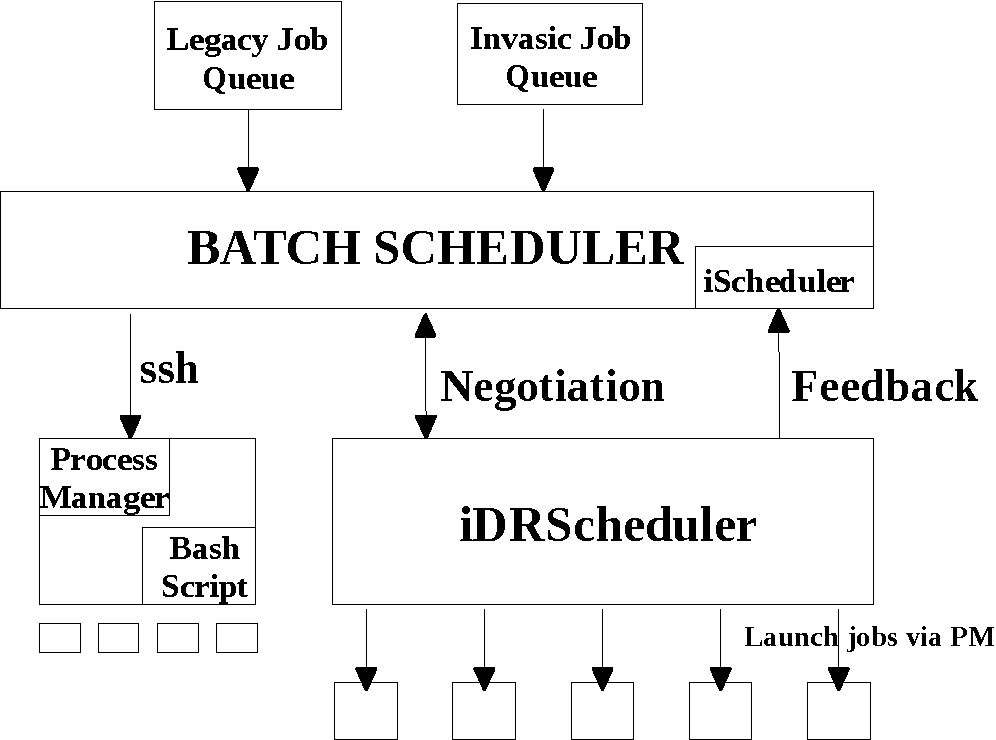
\includegraphics[width=0.8\textwidth, height=60mm]{./figures/architecture.pdf}
\caption{Invasive Resource Management Architecture}
\label{fig:1}
\end{figure}
\noindent
The above figure illustrates the proposed invasive resource management architecture. In addition to a job queue for legacy static jobs, we now have an additional job queue for invasic jobs. The existing batch scheduler needs to be extended in order to schedule these new type of Invasic Jobs and a new component called \textbf{\textit{Invasic Scheduler (iScheduler)}} is responsible for this. In contrast to modifying an existing system to support Invasive Resource Management, a new component called \textbf{\textit{Invasive Distributed Run Time Scheduler (iDRScheduler)}} is proposed which sits between the Batch Scheduler and Process Manager. The objective of such a multi-level approach is to avoid modifying the existing system which will be a substantially large effort and rather have an independent component that caters specifically to Invasic Jobs. It is responsible for managing the resources present in the Invasic paritition used specifically for running Invasic Jobs. With this approach, the existing Legacy Jobs can be served via the existing batch scheduler and the new Invasic Jobs can be served by via iScheduler and iDRScheduler. iDRScheduler talks to the iScheduler via a protocol called the Negotiation protocol to receive Invasic Jobs dispatched from iScheduler which it then launches for execution by performing some run time scheduling like pinning of jobs, expand/shrink etc.\\ \par
\noindent
The new components proposed in the architecture help achieve the objective of supporting dynamic resource management for invasic applications. iScheduler is responsible for scheduling Invasic Jobs. The scheduling decisions are communicated via negotiation protocol to iDRScheduler and these decisions are basically job(s) selected via a scheduling algorithm to be submitted for execution. The decisions will be made on the basis of Resource Offers sent by iDRScheduler which creates these resource offers based on the state of the partition. Upon receiving a resource offer, iScheduler will either accept it by selecting jobs from the queue that can be mapped to this offer or reject it. A Resource Offer can represent real or virtual resources because the iDRScheduler can also present a virtual view of resources in the hope of getting a mapping of jobs to offer that is more suitable to satisfy its local metrics such as resource utilization, power stability, energy efficiency etc. It can either accept or reject the mapping received from iScheduler. Similar to iDRScheduler, the iScheduler makes its decisions to optimize for certain local metrics such as high job throughput, reduced job waiting times, deadlines, priorities etc. This highlights the mismatching policies/metrics for which both the iDRScheduler and iScheduler make their decisions on and hence both will be involved in some kind of a negotiation via the protocol to reach a common agreement. iDRScheduler is an independent entity introduced with the purpose of inter-operating with existing batch systems rather than replacing them with an entirely new one. It may be possible that in the future this component will not be a separate entitiy but will be built into the batch system itself.\\ \par
\noindent
\textbf{\textit{Shrink/Expand Strategies: }}There are several strategies one may employ to tackle adaptive applications during runtime and take decisions that can lead to higher system utilisation, energy efficiency etc.:
\begin{itemize} 
\item Let us consider that at any given point of time there are some Invasic Jobs running in the system. If the parallel runtime environment is able to anticipate that in the near future, there may be a large window of free resources available because some applications may shrink according to a prediction of their scalability behavior with the help of run time profiling and collected performance data then iDRScheduler can provide a resource offer to iScheduler. This offer can specify a virtual list of nodes more than what is available in order to get a mapping of jobs. These jobs can then be shrunk and fit into the existing space of resources with the knowledge that they may be able to expand later.
\item Another scenario is where there is an anticipation of a smaller window of resources in the future because some of the currently running applications may expand. In such a case iDRScheduler will provide a resource offer to iScheduler with a virtual list of nodes smaller than what is currently available in order to get a mapping of jobs. These jobs can be then be expanded and fit into the existing space of resources with the knowledge that they may have to shrink later.
\item The third variation could be the case where the runtime anticipates the state of resources to remain the same as the current state for the near future since none of the running applications may expand or shrink. In such a scenario iDRScheduler will send a resource offer that is a list of nodes which is exactly the same as the available resources to iScheduler in order to get a mapping of jobs. These jobs can then be fit into the space of resources available as it is without expanding/shrinking them. 
\end{itemize}
\section{Master Thesis}
The focus of this Master Thesis is to extend the early prototype developed as a part of the guided research in the last few months. It will now give concrete meanings to the negotiation protocol, defining the format of the invasic job records, its constraints, definition of resource offers, feedback reports and most important of all to investigate and develop an efficient job scheduling algorithm at the iScheduler level. Following this closely from the Guided Research would be to continue having an automated testing in place that will help in simulating a workload of jobs, testing the job scheduling algorithm for its correctness, evaluating and analysing the performance of such a prototype for various metrics. Given below is a tentative plan of the activities proposed monthwise starting from November $15$ till May $15$ to be carried out for the duration of 6 months in this Master Thesis.\par
\subsection{Tentative Plan}
\begin{itemize}
\item Literature survey for current/recent related work on batch job scheduling from research groups focusing on problems in the areas of batch scheduling, resource management, middleware etc. In addition to this, defining resource offers, invasic job records and job constraints that can come from a pre-computed performance model of an application during its runtime or could be user defined. Once these tasks have been completed, it will follow up with extending the early prototype by the implementation of these ideas and testing them for correctness using the automated testing feature.
\item Integration of the fake iHypervisor with the real iHypervisor by making it as its plugin. Test this integration for all the earlier development using the automated testing feature for correctness. Review, analyse, fix any errors and repeate the process till the integration is stable. Follow this up by understanding the SLURM's existing scheduling algorithms including the recent Machine Learning approach for a possible reuse or enhancement. Define the format of feedback reports sent by iHypervisor and how they can be processed on the iScheduler side including its storage mechanism (possibly using SLURM's existing database functionalities). Implement these ideas in the prototype and test it thoroughly.
\item Investigate and experiment with basic scheduling algorithms first to later proceed with complex ones. Design and implement a sophisticated scheduling algorithm for mapping jobs from Invasic job queue to the resource offers sent by iHypervisor. This algorithm must perform its decision making by also using the collected history/feedback data about many statistical measures provided by iHypervisor periodically.
\item Implementation of the Job Scheduling Algorithm continues for realizing all the necessary requirements as proposed earlier till it has been successfully implemented and later followed by a lot of functional testing.
\item Test the full prototype along with the other component iHypervisor (Including its Run Time scheduling and Invasive Resource Management) for simple to complex workloads (emulating a queue of invasic jobs possibly including legacy static jobs). Testing also needs to be done with real Invasic applications developed by the \textit{Chair Of Scientific Computing}. Find issues/errors, review, analyse, correct and repeat the process till it is stable and then collect all the results necessary.
\item Coming up with the draft version of the Master Thesis Report followed by reviews, corrections. This process is repeated till the final version is decided. Also prepare the slides for the Master thesis to present them at a later stage.
\end{itemize}
\noindent
\\The above timeline highlights a tentative plan for the activities to be taken up during the Master Thesis and the $6$ items above correspond to these $6$ months of the Thesis in a chronological order. The steps may overlap or shift depending on the progress but the same overall structure will be followed for the Thesis. It will also include in parallel small amounts of documentation in the report as and when necessary during the $6$ month period and not necessarily everything at the end.\par

\section{Motivation}

\section{Document Structure}
This is end of the first section which gave an introduction to this Master Thesis and the kind of problem it deals with. The rest of this report is organized as follows:
\begin{itemize}
\item \textbf{\textit{Modeling:}} This section will explain in brief on how the DNDP will be mathematically formulated using a bilevel linear program with all its contraints, decision variables and objective function. It will explain the approach to approximate the non-linear objective function of the inner problem of DNDP which is TAP and an introduction to metaheuristics that will be used to solve such kind of a combinatorial optimization problem.
\item \textbf{\textit{Genetic Algorithm:}} This section will dive into the details of the genetic algorithm that includes all the important aspects which fall under GA that needs to be tackled in order to come up with a correct implementation yielding good performance. It will explain in detail some of the many choices one has for implementation during every step of GA.
\item \textbf{\textit{Implementation:}} This section will illustrate with the help of a flow chart the high level view of the GA implementation followed by some pseudo codes to demonstrate in a simple language the implementation details of the inner workings of GA.
\item \textbf{\textit{Experiments and Visualization:}} This section will present all the results of the experiments conducted on different types(sizes) of datasets using the implemented GA in the form of tables. It will also mention in brief some of the observations and inferences that have been drawn by looking at these results.
\item \textbf{\textit{Conclusion:}} This section concludes the report on this project with a highlight of what was successfully achieved along with the possible scope of what can be done as a part of future research work. This is followed by a list of some useful references that played an important role in the understanding of many of the concepts towards the realization of this project.
\end{itemize}

\chapter{Related Work}\label{chapter:related work}
The problem of job scheduling for adaptive applications as introduced in the previous chapter is really an intersection of many different problems. In this section, we will look at the some of the relevant work that has happened in the past with respect to batch job scheduling and also briefly look at a subset of the relevant work that has happened with resource-aware programming models and runtime scheduling.\\ \\
%%%%%%%%%%
Substantial amount of work has been done in exploring efficient resource management and scheduling for HPC systems in the past focusing on rigid and moldable jobs. There has been growing interest in the recent years to explore dynamic resource management and scheduling techniques due to the increasing complexity of applications, ex: Scientific applications utilizing Adapative Mesh Refinement(AMR) techniques change their working set size as the mesh is refined/coarsened. Dynamically allocating resources to such applications at runtime or other applications which are potentially scalable has the potential to improve resource utilization, energy efficiency, fault tolerance and a host of other metrics\cite{abhishek}\cite{osman}. Wolf.et.al\cite{felix} demonstrated such a dynamic resource management approach for supporting evolving jobs<ref to section no.> by extending the Torque / Maui Batch System to allow dynamic allocations and a dynamic fairness strategy implemented in the Maui Scheduler to efficiently service static and dynamic allocations. Their results showed reduced turnaround and waiting times for applications, while increasing system utilization and throughput. Wolf.et.al\cite{laxmikant} also proposed an extension to this work to further support malleable<ref to section no.> type of jobs with the help of a communication protocol between the Batch System and the Charm++ runtime which enables the malleability of applications. In combination with their earlier work, The Scheduler now supported a mix of jobs with different types such as rigid, malleable and evolving.\\ \\
%%%%%%%%%%%
In contrast to the research works mentioned above that focused on the Charm++ programming model, there have been several efforts directed towards the MPI programming model\cite{georgiou}\cite{travis}\cite{gladys}\cite{gonzalo}\cite{martin} some of which explored on how to first provide such an adaptive behavior on MPI applications and some on how to support the same with the help of libraries, resource management systems\cite{klein} etc. In the current collaborative research project earlier efforts were directed towards supporting such adaptive programming paradigms in shared memory programming model such as openMP\cite{andreas} and work was also done in MPI\cite{isaias}. The ongoing efforts in this project is to now continue forward in the direction of MPI but to approach the problem vertically at different levels of abstraction such as the programming model, middleware and runtime tuning of applications.\\ \\
%%%%%%%%%
This thesis will mainly focus on the middleware part of this solution stack to support adaptive applications in future HPC systems. Middlewares provide job scheduling for HPC systems and job scheduling has always remained a very active area of research both for theoretical purposes and for practical systems. The most widely used and proven technique running in most of the HPC systems today is backfilling. Backfilling was first developed by lifka\cite{david} for the Argonne National Laboratory's IBM SP system to address the need for a new scheduling system on supercomputers and was named as \textbf{EASY}(Extensible Argonne Scheduling System). Feitelson.et.al\cite{ahuva} proposed an extension to backfilling by providing a reservation for every job that could not be started and allowing lower priority jobs from behind in the queue to start if they would not delay these reservations. This was called as \textbf{\textit{Conservative Backfilling}} whereas the one proposed by lifka was called \textbf{\textit{Aggressive Backfilling}} as it provided a reservation to the job only at the front of the queue. Feitelson.et.al\cite{dror} came up with a new approach to backfilling algorithm where a set of jobs from the job queue are looked at once for making a scheduling decision using dynamic programming instead of traversing the queue one job at a time. The claim was that this resulted in better packing of jobs resulting in higher utilization, reduced mean response time and mean slowdown of all jobs. This scheduler was named as \textbf{\textit{LOS(Lookahead Optimizing Scheduler)}}.\\ \\
%%%%%%%%%%
In addition to the standard batch job scheduling for rigid jobs, efforts have also been made in the direction of supporting moldable jobs. Cirne.et.al\cite{wcirne} proposed \textbf{SA(Supercomputer AppLes - Application level scheduler)} that would select on behalf of the user, the appropriate size for a given job from its available sizes. This decision was made based on the state of the resources, job characteristics etc to minimize turnaround time. Sadayappan.et.al\cite{sabin}\cite{srividya}\cite{sudha} proposed several works for moldable scheduling of parallel jobs by using different policies like fair-share, overbooking, and finally considering job's efficiency also in determining the best partition size for the job. They developed an iterative algorithm in order to make the appropriate choice of values for overbooking and efficiency which is inturn based on the scalability characteristics of the job mix.\\ \\
%%%%%%%%
Traditionally, Batch Systems have had both batch and runtime scheduling merged together into a single component. In this work, we explore the idea of separating the two concerns into different components for providing a dynamic and flexible scheduling functionality. Such a multi-level approach has usually been observed in the grid and cloud based infrastructures\cite{kwang}\cite{kurowski}\cite{streit}. These infrastructures are distributed geographically and employ a local resource manager and scheduler at each of these locations and all of these locations are coordinating by a single centralized broker / service provider. The broker usually engages in some sort of a negotiation\cite{oliver}\cite{roland}\cite{viktor}\cite{rizos} with the different locations / resource providers / sites for availability of resources in order to make the best possible decision for serving its users.

\chapter{Invasive Computing}
\label{chapter:invasive computing}
Invasive Computing is a novel paradigm for designing and programming future parallel systems. Decreasing feature sizes are motivating a redesign of multi million transistor system-on-chip architectures. This can lead to a dramatic increase in the rates of temporary and permanent faults as well as feature variations. SoCs with 1000 or more processors on a single chip in the year 2020 are foreseen, hence static and central management concepts to control the execution of all resources are no longer appropriate. Invasive Computing allows a program to be resource-aware by which it can explore and dynamically spread its computations to neighbour processors in a phase called as \textbf{\textit{invade}}, then to execute portions of code of high parallelism degree in parallel based on the available invasible region in a given multi-processor architecture in a phase called as \textbf{\textit{infect}}. Later, once the degree of parallelism should be lower again or if it terminates, the program may enter a \textbf{\textit{retreat}} phase where it can deallocate resources and resume execution again, for example, on a single processor. With the help of such resource awareness, the program has the ability to self-organise itself and be immune to faults, feature variations, be highly scalable, show performance gain and record a higher resource utilization metric.\\ \\
This concept would require not just new programming concepts, languages, compilers and operating systems but a radical change in the architectural design of MPSoCs(\textit{Multi-Processor Systems-On-a-Chip}) so as to efficiently support invasion, infection and retreat operations. Some of the main motivations behind the idea of invasive computing are enumerated below:
\begin{itemize}
\item \textbf{\textit{Programmability}} How to map algorithms and programs to 1000 processors or more and how to benefit from the massive parallelism available by tolerating manufacturing defects, feature variations etc.
\item \textbf{\textit{Adaptivity}} Modern applications have unpredictable resource requirements most of which may not be known at compile-time. In addition to this, when different applications are running on a single chip, resource distribution will have to happen dynamically keeping up a high resource utilization and performance. These factors show the need for some sort of hardware / software reconfigurability of the MPSoC.
\item \textbf{\textit{Scalability}} How to efficiently run algorithms and programs on different number of resources?
\item \textbf{\textit{Physical Constraints}} Heat dissipation will be a major bottleneck. Intelligent methods and architectural support to run algorithms at different speeds to exploit parallelism under power reduction is needed.
\item \textbf{\textit{Reliability and Fault-Tolerance}} Applications must be immune to temporal or permanent faults that may be caused due to manufacturing defects, feature variations, degradation etc. This especially has a higher likelihood to happen in the case of future MPSoCs.
%%%%%%%
\end{itemize}
The paradigm of invasive computing offers a new perspective for programming large scale HPC systems. Current resource management systems manage resources via static partitioning among parallel jobs. This is a very rigid approach considering that an application will then be limited to a fixed amount of parallelism it can utilize. This, however, will not be beneficial especially in the case of future exascale systems where if one needs to derive maximum performance then the maximum number of resources will have to be allocated. The application can benefit from invasive programming during certain phases of its runtime by running at maximum parallelism and in the remaining time it can run at a lower parallelism.\\ \\
%%%%%%%
Another motivation is for a specific classes of applications like multi-grid and adaptive grid. Multi-grid applications work on multiple grid levels ranging from fine to coarse grids. On fine grids, more resources could yield better performance and efficiency, whereas on coarse grids fewer resources would be sufficient. In the case of adaptive grid applications, the grid is dynamically refined according to the current solution and the application may go through different levels of parallelism in different phases.\\ \\
%%%%%%%
Scaling the systems to exaflop level would consume significantly more power that would very likely cross a gigawatt, roughly the output of Hoover Dam. Reducing the power requirement by a factor of atleast 100 is a challenge for future hardware and software technologies. Invasive computing concept with invasive programming models combined with intelligent resource management and flexible scheduling mechanisms can possibly help in addressing this challenge.\\ \\
%%%%%%%
Coping with run-time errors would be another major challenge. Due to design and power constraints, the clock frequency is unlikely to change and feature sizes would continue to decrease as per moore's law for the next few years. By 2020, it is envisaged that exascale systems can possibly have approximately one billion processing elements. An immediate consequence is that the frequency of errors will increase while timely identification and correction of errors would be much more difficult. Fault tolerance would be one of the most important challenges in this regard.\\ \\
%%%%%%%
Exploiting massive parallelism for current and emerging scientific applications would also be another major challenge.
\section{Traditional Resource Management}
The role of a resource manager is to act like a \textit{glue} for a parallel computer to execute parallel jobs. It should make a parallel computer as easy to use as almost a personal computer. MPI would typically be used to manage communications within the parallel program. A resource manager allocates resources within a cluster, launches and otherwise manages the jobs. Some of the examples of widely used open source as well as commercial resource managers are \textbf{SLURM, TORQUE, OMEGA, IBM Platform LSF} etc. Together with a scheduler it is termed as a \textbf{\textit{Batch System}}. The Batch System serves as a middleware for managing supercomputing resources. The combination of \textit{Scheduler}$+$\textit{Resource Manager} makes it possible to run parallel jobs.\par
\noindent
\\
The role of a job scheduler is to manage queue(s) of work when there is more work than resources. It supports complex scheduling algorithms which are optimized for network topology, energy efficiency, fair share scheduling, advanced reservations, preemption, gang scheduling(time-slicing jobs) etc. It also supports resource limits(by queue, user, group, etc.). Many batch systems provide both resource management and job scheduling within a single product (e.g. LSF) while others use distinct products(e.g. Torque resource manager and Moab job scheduler). Some other examples of job scheduling systems are \textbf{LoadLeveler, OAR, Maui, SLURM} etc.
%%%%%%
\subsection{Classification}
The process of computing a schedule may be done by a queueing or planning based scheduler. A \textit{Schedule} is computed for the job requests that are present in the job queue. Every request contains information such as the number of requested resources and a duration for how long the resources are requested for. A job consists of a request and some additional information about the associated application. These additional details could be the following: information about the processing environment (e. g. MPI or PVM), file I/O and redirection of stdout and stderr streams, the path and executable of the application, or startup parameters for the application etc. There can also be some reservation requests present. These request for resources at a specified time for a given duration. Once the scheduler accepts such a request, it is a reservation and those exact resources are then blocked for that specified time and are unavailable for any scheduling purposes.\\ \\
%%%%%%
The classification of resource management systems is based on the planned time frame [42]. Queuing systems try to utilize the currently available resources in order to satisfy the job requests. Future resource planning for all the pending requests is not done. Hence, the pending requests have no proposed start times. Planning systems in contrast, plan for the present and the future. Planned start times are assigned to all requests and a complete schedule about the future resource usage is computed.\\ \\
%%%%%%%%%%%%
\textbf{\textit{Queuing Systems }} These systems have several queues with different limits on the number of requested resources and the runtime limit for the job. Jobs within a queue are ordered according to a scheduling policy, e. g. FCFS (first come, first serve). Queues might be activated only for specific times (e. g. prime time, non prime time, or weekend). The task of a queuing system is to assign free resources to waiting requests. The highest prioritized request is always the queue head. If it is possible to start more than one queue head, further criteria like queue priority or best fit (e. g. leaving less resources idle) are used to select a request. There might also exist a high priority queue whose jobs are preferred at any time. If not enough resources are available to start any of the queue heads, the system waits until enough resources become available. These idle resources may be utilized with less prioritized requests by backfilling mechanisms.\\ \\
%%%%%%%
In queuing systems, no information about future job starts are available. Consequently guarantees can not be given and resources can not be reserved in advance. Resource reservation will have to be done manually by the administrative staff. Usually high priority queues combined with dummy jobs for delaying other jobs are used. Job requests also come with run time limits. A longer run time than the limit of the queue is not allowed and the resource management system usually kills such jobs. If the associated application still needs more CPU time, the application has to be checkpointed and later restarted by the user. Also, if a job runs for more than the run time limit it specified, then the system will usually kill such a job.\\ \\
%%%%%%%%%
\textbf{\textit{Planning Systems }}Planning systems schedule for the present and future. They assign start times to all requests and a full schedule is generated. Runtime estimates for jobs are mandatory for this planning. With this knowledge advanced reservations are easily made possible. The re-planning process is the key element of a planning system. Each time a new request is submitted or a running request ends before it was estimated to end, a new schedule has to be computed and this function is invoked. At the beginning of a re-plan, All pending requests are sorted according to a scheduling policy in addition to clearing their previous planned start times. All the pending requests are then re-inserted at the earliest possible start time in the schedule. After this step each request is assigned a planned start and end time.\\ \\
%%%%%%%%%
As planning systems work with a full schedule and assign start times to all requests, resource usage is guaranteed and advanced reservations are possible. A reservation usually comes with a given start time or if the end time is given the start time is computed with the estimated run time. When the reservation request is submitted the scheduler checks with the current schedule, whether the reservation can be made or not. That is the amount of requested resources is available from the start time and throughout the complete estimated duration. If the reservation is accepted it is stored in an extra list for accepted reservations. During the re-planning process this list is processed before the list of standard job requests which can float around in the schedule. It does not have to be sorted as all reservations are accepted and therefore generate no conflicts in the schedule.\\ \\
%%%%%%%%%
One drawback in a planning system is the cost of scheduling. Furthermore, The usage of reservations should be monitored as users may misuse this facility without really needing it. This can be avoided by automatically releasing unused reservations after a specific idle time.
%%%%%%%%%
\subsection{Job Scheduling}
Typical resource management systems store job requests in list-like structures. A scheduling policy consists of two parts: inserting a new request in the data structure at its submission and taking requests out during the scheduling. Different sorting criteria are used for inserting new requests and some examples are (either in increasing or decreasing order):
\begin{itemize}
\item by arrival time: FCFS (first come first serve) uses an increasing order and FCFS is probably the most known and used scheduling policy as it simply appends new requests at the end of the queue. With this example the term fairness is described [79]. 
\item by duration: Both increasing and decreasing orders are used. Sorting by increasing order leads to SJF (shortest job first) respectively FFIH (first fit increasing height). Accordingly LJF (longest job first) and FFDH (first fit decreasing height) sort by decreasing run time. In an on-line scenario this requires duration estimates, as the actual duration of jobs are not known at submission time. SJF and LJF are both not fair, as very long (SJF) and short (LJF) jobs potentially wait forever. LJF is commonly known for improving the utilization of a machine.
\item by area: The jobs area is the product of the width (requested resources) and length (estimated duration). FFIA (first fit increasing area) is used in the SMART algorithm (Scheduling to Minimize Average Response Time) [91, 76]. 
\item by given job weights: Jobs may come with weights which are used for sorting. Job weights consist of user or system given weights or a combination of both. For example: all jobs receive default weights of one and only very important jobs receive higher weights, i. e. they are scheduled prior to other jobs.
\item by the Smith ratio: The Smith ratio of a job is defined by weight area and is used in the PSRS (Preemptive Smith Ratio Scheduling) algorithm [75].
\item by many others: e. g. number of requested resources, current slowdown, ...
\end{itemize}

In the scheduling process, Jobs are taken out of the ordered data structure for either a direct start in queuing systems or for placing the job in a full schedule (planning system):
\begin{itemize}
\item front: The first job in the data structure is always processed. Most scheduling policies use this approach as only with this a sorting policy makes sense. FCFS, SJF, and LJF use this approach.
\item first fit: The first job is taken, that matches the search constraints, i. e. requests equal or less resources than currently free.
\item best fit: All jobs are tested to see whether they can be scheduled. According to a quality criterion the best suited job is chosen. Commonly the job which leaves the least resources idle in order to increase the utilization is chosen. If more than one job is best suited an additional rule is required, e. g. always take the first, the longest/shortest job, or the job with the most weight.
\item next fit: The SMART algorithm uses this approach in a special case (NFIW) [91, 76].
\end{itemize}
In general, all combinations are possible but only a few are applicable in practice.\\ \\
%%%%%%%
If fairness in common sense has to be met, i. e. the starting order equals the arrival order, only the combination of sorting by increasing arrival time and always processing the front of the job structure can be used. All other combinations do not generate fair schedules. However, such a fair scheduler is not very efficient, as jobs usually have to wait until enough free resources are available. Therefore, basic scheduling policies are extended by backfilling, a method to avoid excessive idleness of resources. Backfilling has become a standard in modern resource management systems today. If requests are scheduled out of their sorting order by first or best fit, some form of backfilling is carried out.\\ \\
%%%%%
\textbf{\textit{EASY Backfilling }}The default algorithms used by job schedulers for parallel supercomputers employ a straightforward version of variable partitioning. (This means space-slicing with static-partitioning, where users specify the number of processors required by their jobs upon submittal.) In essence, schedulers select jobs for execution in first-come first-served (FCFS) order, and run each job to completion, in batch mode. The problem with this simplistic approach is that it causes significant fragmentation, as jobs with arbitrary sizes/arrivals do not pack perfectly. Specifically, if the first queued job requires many processors, it may have to wait a long time until enough are freed. During this time, processors stand idle as they accumulate, despite the fact there may very well be enough of them to accommodate the requirements of other, smaller, waiting jobs.\\ \\
%%%%%
To solve the problem, most schedulers therefore employ the following algorithm. Whenever the system status changes (job arrivals or terminations), the scheduler scans the queue of waiting jobs in order of arrival (FCFS) and starts the traversed jobs if enough processors are available. Upon reaching the first queued job that cannot be started immediately, the scheduler makes a reservation on its behalf for the earliest future-time at which enough free processors would accumulate to allow it to run. This time is also called the \textit{shadow time}. The scheduler then continues to scan the queue for smaller jobs (require fewer processors) that have been waiting less, but can be started immediately without interfering with the reservation. In other words, a job is started out of FCFS order only if it terminates before the shadow time and therefore does not delay the first queued job, or if it uses extra processes that would not be needed by the first queued job. The action of selecting smaller jobs for execution before their time provided they do not violate the reservation constraint is called backfilling.\\ \\
\begin{figure}[!htbp]
\centering
\includegraphics[width=1.0\textwidth, height=45mm]{./figures/"FCFS+Backfilling".pdf}
\caption{FCFS with and without Backfilling}
\label{fig:2}
\end{figure}
This approach was initially developed for the IBM SP1 supercomputer installed at the Argonne National Laboratory as part of EASY (Extensible Argonne Scheduling System), which was the first backfilling scheduler [98].1 The term “EASY” later became a synonym for FCFS with backfilling against a reservation associated with the first queued job. (Other backfill variants are described below.) While the basic concept is extremely simple, a comprehensive study involving 5 supercomputers over a period of 11 years has shown that consistent figures of 40–60 percent average
utilization have gone up to around 70 percent, once backfilling was introduced [79]. Further, in terms of performance, backfilling was shown to be a close second to more sophisticated algorithms that involve preemption (time slicing), migration, and dynamic partitioning [19, 170].\\ \\
%%%%%
\textbf{User Runtime Estimates} The down side of backfilling is that it requires the scheduler to know in advance how long each job will run. This is needed for two reasons:
\begin{itemize}
\item to compute the shadow time for the longest-waiting job (e.g. in the example given in Fig. 1.1, we need to know the runtimes of job 1 and job 2 to determine when their processors will be freed in favor of job 3), and
\item to know if smaller jobs positioned beyond the head of the wait-queue are short enough to be backfilled (we need to make sure backfilling job 4 will not delay job 3, namely, that job 4 will terminate before the shadow time of job 3).
\end{itemize}
Therefore, EASY required users to provide a runtime estimate for all submitted jobs [98], and the practice continues to this day. Importantly, jobs that exceed their estimates are killed, so as not to violate subsequent commitments (the reservation). The combination of simplicity, effectiveness, and FCFS semantics (often perceived as most fair [123]) has made EASY a very attractive and a very popular job scheduling strategy. Nowadays, virtually all major commercial and open-source production schedulers support EASY backfilling.\\ \\
%%%%%%%%%%%
\textbf{Variations on Backfilling} This section briefly mentions some of the various tunable knobs of backfilling algorithms.
\begin{figure}[!htbp]
\centering
\includegraphics[width=1.0\textwidth, height=190mm]{./figures/"BackfillParameters".pdf}
\caption{Backfilling Variations}
\label{fig:3}
\end{figure}
%%%%%%%
\subsection{SLURM}
The prime focus of this work will be on \textbf{SLURM(Simple Linux Utility For Resource Management)} which will be the choice of batch system upon which the support for Invasive Computing will be demonstrated. SLURM is a sophisticated open source batch system written in C whose development started in the year 2002 at Lawrence Livermore National Laboratory as a simple resource manager for Linux Clusters. A few years ago it spawned into an independent firm under the name SchedMD. SLURM has since its inception also evolved into a very capable job scheduler through the use of optional plugins. It is used on many of the world's largest supercomputers and is used by a large fraction of the world's TOP500 Supercomputer list. It supports many UNIX flavors like AIX, Linux, Solaris and is also fault tolerant, highly scalable, and portable.\\ \\
\begin{figure}[!ht]
\centering
\includegraphics[width=1.0\textwidth, height=150mm]{./figures/"SLURM Architecture".pdf}
\caption{SLURM Architecture}
\label{fig:6}
\end{figure}
%%%%%
\noindent
SLURM has a centralized manager called \textbf{\textit{slurmctld}}(controller daemon) that is the main nerve center of SLURM. SLURM operates in a style simlar to the Master-Slave paradigm where the Master is the \textbf{\textit{slurmctld}}. It takes centralized decisions to monitor resources and work. In the event of a failure, there may also be a backup controller. Each of the nodes in the cluster has a daemon running on it called as \textbf{\textit{slurmd}} and these are the slaves. These daemons are started on every node and they are responsible for monitoring them. This can resemble a remote shell: it waits for work from the controller, executes that work, returns status and waits for more work. The \textit{slurmd} daemons provide fault-tolerant hierarchical communications and also are responsible for spawning an additional daemon called \textbf{\textit{slurmstepd}}. The step daemon as it is called is responsible for the node local part of the job step that are the subset of processes running on the local node. A job step in SLURM refers to an application started with the help of srun and its allocated resources. srun could be used independently to launch jobs or one can specify the same within a batch script while using sbatch. \textbf{\textit{srun}} is one of the tools SLURM provides that allows the user to launch interactive jobs on the cluster, \textbf{\textit{sbatch}} to launch batch jobs and several others relating to accounting, job status, cancellation operation etc.\\ \\
The figure x.x shows the high level architecture of SLURM with the interaction between the several of its key components. It also shows the interaction between an MPI application through the PMI(Process Management Interface), \textit{slurmd} daemon of a node and the \textit{slurmstepd}.
\textbf{Plugins} are dynamically linked objects loaded at run time based upon configuration file and/or user options. \ref{fig:6} shows where these plugins fit inside SLURM. Approximately $80$ plugins of different varities are currently available. Some of them are listed below:
\begin{itemize}
\item \textbf{\textit{Accounting storage:}} MySQL, PostgreSQL, textfile.
\item \textbf{\textit{Network Topology:}} 3D-Torus, tree.
\item \textbf{\textit{MPI:}} OpenMPI, MPICH1, MVAPICH, MPICH2, etc.
\end{itemize}
PLugins are typically loaded when the daemon or command starts and persist indefinitely. They provide a level of indirection to a configurable underlying function.
%\begin{figure}[!htbp]
%\centering
%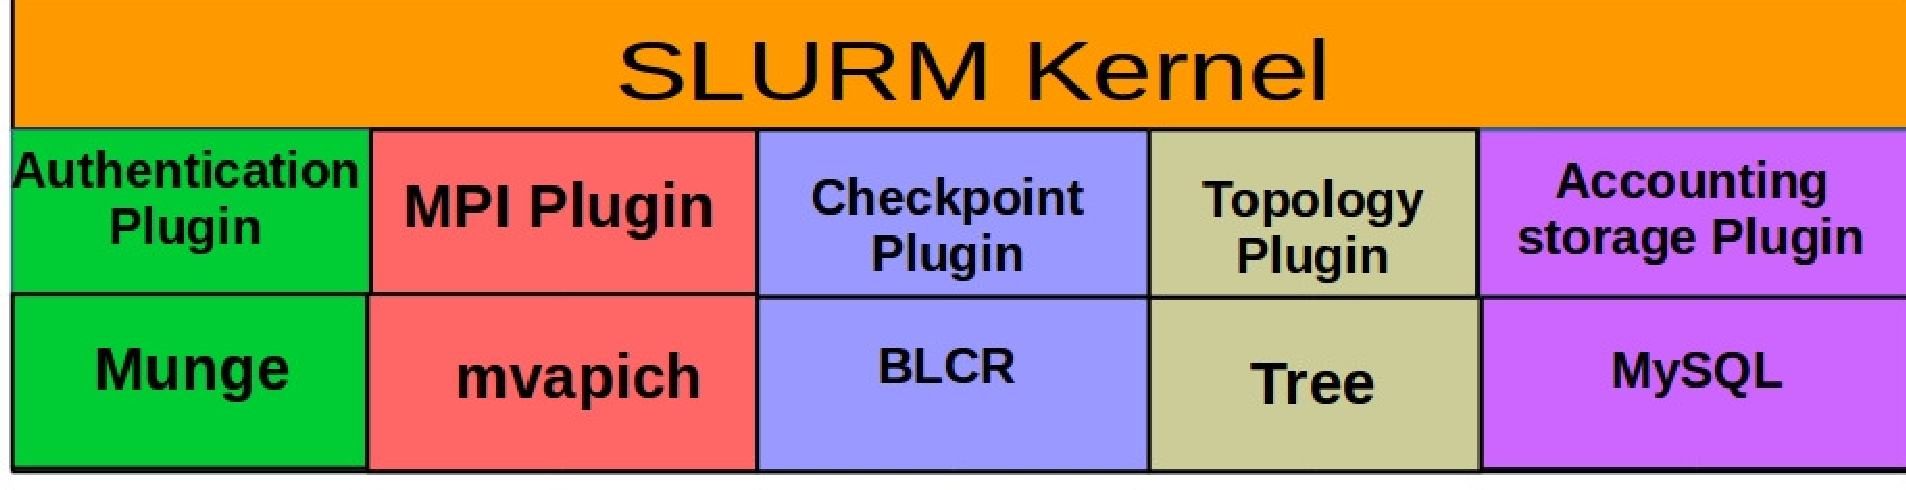
\includegraphics[width=1.0\textwidth]{./figures/plugin.pdf}
%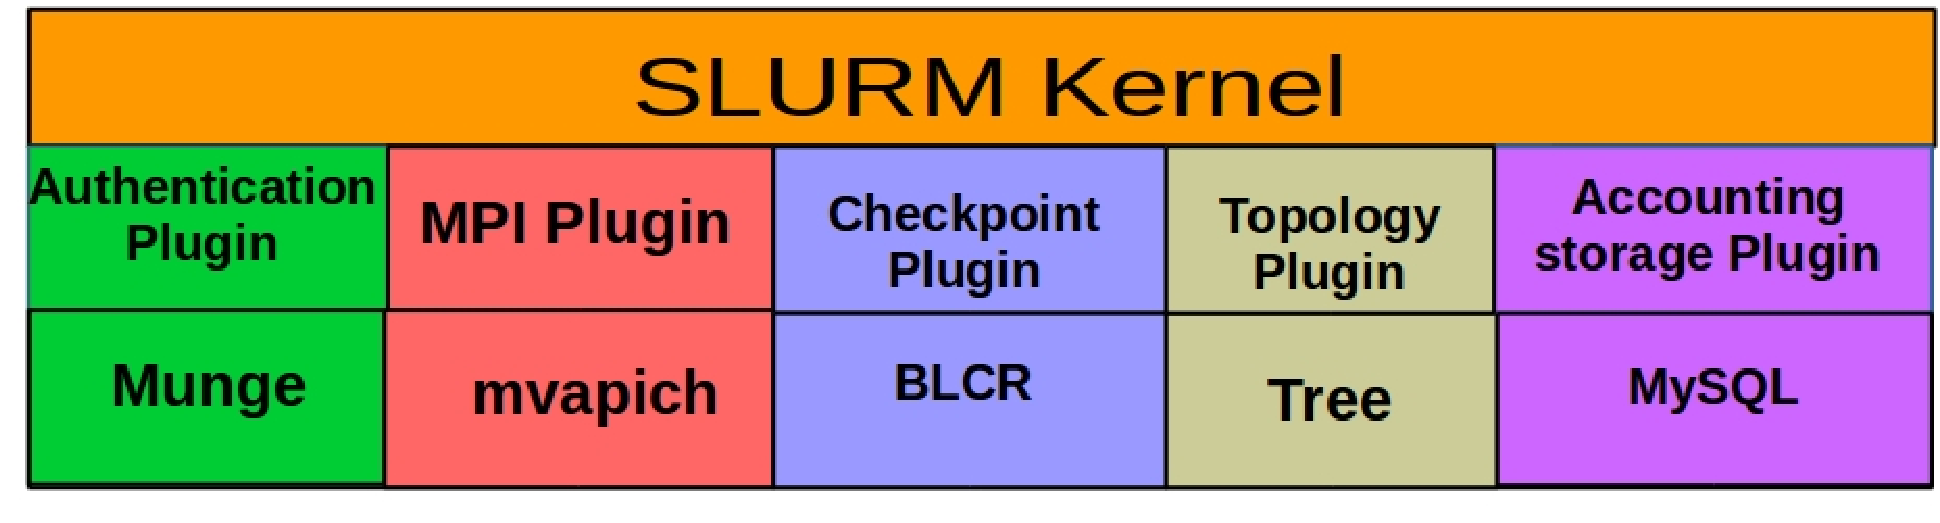
\includegraphics[width=1.0\textwidth]{./figures/plugin.eps}
%\vspace{-0.15in}
%\caption{SLURM with optional Plugins}
%\label{fig:6}
%\end{figure}
%%%%%
\section{Resource Aware Programming}
\subsection{Job Classification}
The throughput of HPC Systems depends not only on efficient job scheduling but also on the type of jobs forming the workload. As defined by Feitelson, and Rudolph, Jobs can be classified into four categories based on their flexibility:
\begin{itemize}
\item \textbf{\textit{Rigid Job:}} Requires a fixed number of resources throughout its execution.
\item \textbf{\textit{Moldable Job: }} The resource requirement of the job can be molded or modified by the batch system before starting the job(e.g. to effectively fit alongside other rigid jobs). Once started its resource set cannot be changed anymore.
\item \textbf{\textit{Evolving Job: }} These kind of jobs request for resource expansion or shrinkage during their execution. Applications that use Multi-Scale Analysis or Adaptive Mesh Refinement (AMR) exhibit this kind of behavior typically due to unexpected increases in computations or having reached hardware limits (e.g. memory) on a node.
\item \textbf{\textit{Malleable Job: }} The expansion and shrinkage of resources are initiated by the batch system in contrast to the evolving jobs. The application adapts itself to the changing resource set.
\end{itemize}
The first two types fall into the category of what is called as the static allocation since the allocation of rigid and moldable jobs must be finalized before the job starts. Whereas, the last two types fall under the category of dynamic allocation since this property of expanding or shrinking evolving and malleable jobs (together termed adaptive jobs) happens at runtime. Adaptive Jobs hold a strong potential to obtain high system performance. Batch systems can substantially improve the system utilization, throughput and response times with efficient shrink/expand strategies for running jobs that are adaptive. Similarly, applications also profit when expanded with additional resources as this can increase application speedup and improve load balance across the job\textquotesingle s resource set.
%%%%%
\subsection{Invasive Programming Models}
In this section, we will briefly look into the details of the earlier invasive extensions done to OpenMP and MPI done as a part of this ongoing research project. This will give us an insight into the earlier approach taken towards realizing such resource-aware programming models and also serve as a prelude to the approach currently undertaken. These invasic extensions provide us with a new parallel programming model that allows us to implement resource aware programs. Depending on the semantics of these new extensions, the resulting application can either be evolving(application dictates the changes to its resource set) or a malleable job(resource manager dictates the change in resources to which the application must adapt). Resource awareness could mean that either the program can allocate or free resources according to the amount of available parallelism / the dynamic size of the data or it could mean that it can adapt to the available resources for execution.\\ \\
%%%%%%%%%
In the context of invasive computing, parallel applications are resource aware and will invade or retreat from resources depending on their availability and on the load imbalances encountered during their runtime. To support this, some form of dynamic process management of the parallel application is necessary. And, in order to realize this in practice, the most basic requirement would be the need for a library that will serve as an application programming interface for programmers to implement such invasic applications that are capable of adapting to a changing set of resources. This requirement needs to be complemented by the extension of the resource management systems which would need to allocate / deallocate resources and coordinate with the library to allow for such adaptive operations of an invasive parallel application.\\ \\
\textbf{iOMP}\\
The OpenMP parallel programming model for shared memory systems was extended to support the programming of resource aware applications and is named as Invasive OpenMP or iOMP. OpenMP is implemented as a set of compiler directives, library routines and environment variables. Parallelization is based on directives inserted into the application's source code to define parallel regions that are executed in parallel using a fork-join parallelization model. The parallel region would then be executed by a team of threads whereas the sequential region would be executed by a single master thread. There are different ways to control the number of threads in a parallel region and the most common approach is through the environment variable, or through OpenMP library call or as an additional clause in its directives. It has language bindings for C, C++ and Fortran. iOMP has been implemented as a library in C++ using an object oriented approach and provides two important methods / operations available in its class \textbf{\textit{Claim}}:
%%%%
\begin{itemize}
\item \textbf{\textit{Invade}}: This operation allocates additional resources / PE's. A constraint parameter passed as an argument to this operation specifies the details such as which resources and how many of them [range] are additionally required from the resource manager.
\item \textbf{\textit{Retreat}}: This operations deallocates resources / PE's. A constraint parameter passed as an argument to this operation specifies the details such as which resources and how many of them must be freed to the resource manager.
\end{itemize}
%%%%%%
iOMP follows a similar terminology as mentioned in section x.x.x for X10 in invasive computing. A \textit{Claim}(not the C++ Class) in iOMP refers to all the resources / PE's allocated to the application. This means that an iOMP program will always have a single claim. Initially, the claim size is $1$ but it will increase and decrease during the runtime of the application. The constraint parameter mentioned before also allows the programmer to specify several other constraints such as memory, pinning strategy, architecture specific optimizations etc. Below is a small snippet of code from the paper that shows an example of iOMP program.
\begin{lstlisting}[frame=single]
int main() 
{
	Claim claim;
	int sum = 0;
	/* Acquire resources according to the given constraints */
	claim.invade(PEQuantity(1, 3));
	
	/* Executing a parallel for loop on the given resources */
	#pragma omp for reduce reduction(+:sum)
	for (int i=0; i < 100000; i++)
		sum += i;
	
	/* Free resources and delete pinning */
	claim.retreat();
}		
\end{lstlisting}
%%%%%%%%
As another important part of the iOMP implementation,  A resource manager has also been implemented. This has a global view of the resources in the shared memory system and acts like a server to every other running application that are its clients. Every client-server communication happens over a message queue. The resource manager handles the redistribution of the resources over time to all running applications based on their invade / retreat operations.\\ \\
%%%%%%%%
%%%%%%%%
\textbf{iMPI}\\
Similar to \textbf{iOMP}, previous research effort in this project was also directed towards extending parallel programming models for distributed memory systems. iMPI which stands for Invasive MPI is an extension to the MPI library that can support resource aware programming. The Single-chip Cloud Computer(SCC) from Intel Labs was an experimental CPU that integrates 48 cores and is basically a distributed memory system on the chip. This hardware platform along with its interesting memory features was used in order to evaluate this invasive programming model.\\ \\
%%%%%%
Message Passing has for long remained the dominant programming model for distributed memory systems. MPI stands for Message Passing Interface. It is a standardized and portable message passing system designed to function on a wide variety of parallel computers. It defines the syntax and semantics of a core of library routines for writing portable programs in C, C++ and Fortran. It implements a message passing type of parallel programming model where the application consists of a set of processes with separate address spaces. The processes exchange messages by explicit send/receive operations. There are several well-tested and efficient implementations of MPI, many of which are open-source or in the public domain. These have fostered the development of a parallel software industry, and encouraged development of portable and scalable large-scale parallel applications. Some of the most popular and widely used open-source implementations of MPI standard are MPICH and OpenMPI. LAM / MPI was the predecessor of OpenMPI and was another early MPI implementation. There are also commercial implementations from HP, Intel and Microsoft.\\  \\
%%%%%%
The following are the invasive extensions to MPI:
\begin{itemize}
\item \textbf{\textit{MPI\_Comm\_invade}}: The main purpose of this operation is to reserve resources and for this it looks into what resources are currently available and invades them.
\item \textbf{\textit{MPI\_Comm\_infect}}: This operation is used by the application to specify the total number of cores to infect and which ones are preferred. This number can be less than or equal to the total number of cores that were reserved by the invade operation. 
\item \textbf{\textit{MPI\_Comm\_retreat}}: This operation does the reverse of the invade+infect sequence. Instead of reserving and claiming resources, it returns them so that other invasive applications can claim them.
\end{itemize}
The above extensions were based on the MPICH2 library. A new process manager called \textbf{Invasive Process Manager(IPM)} was also developed as a part of the iMPI implementation. It was responsible for launching of the MPI jobs, as well as spawn operations(invade+infect) with low latency and functionality for resource awareness.\\ \\
\textbf{Other Resource-Aware Programming Models}
%%%%%%%%%
%%%%%%%%%
\section{Invasive Resource Management}
In this section, we will look at the latest extensions done to the MPI library for programming on HPC systems like clusters, supercomputers etc and also the extensions done to a resource managers managing these HPC systems. This is in contrast to the earlier version of the iMPI which was targeted towards the Intel SCC platform. The MPI and Resource Manager extensions are not accomplished as a part of this thesis but are essential to be described here in order to get the right context for adaptive applications and their scheduling.
\subsection{Invasive MPI}
Traditionally MPI applications are static in nature which means that they are executed with a fixed number of processes. Dynamic process support is available through the MPI spawn and its related operations. The spawn operation creates new processes in a separate child process group, whereas the callers belong to the parent process group. This is a blocking operation where the processes in the parent process group block till the operation is completed. The two process groups are connected to each other via an intercommunicator which is generated during this spawn operation and returned to the application. This intercommunicator can then be used to reach children processes from the parent's process group, or parent processes from the children's process group. Another form of spawn is the multiple version which allows the callers to specify multiple binaries to start as children processes and few other related operations with their own usefulness.\\ \\
\noindent
Although the MPI standard provides support for dynamic processes, it suffers from many drawbacks as mentioned below:
\begin{itemize}
\item The spawn operations are collective operations and are synchronous across both the parent and child process groups. This effects performance and can induce delays of several seconds.
\item These operations produce intercommunicators based on disjoint process groups. Subsequent creation of processes result in multiple disjoint process groups. These factors can complicate the development of an MPI application.
\item Destruction of processes can be done only on entire process groups. This shortcoming limits the granularity of operations that can be carried out as only entire process groups can be destroyed. This also limits the location of the resources that the application can release at runtime.
\item The processes created with spawn are typically run in the same unmodified resource allocation. Although, not a limitation of the standard itself, but, lack of support from resource manager will result in limiting the usefulness of this spawn operation by not changing the physical resource set of the application.
\end{itemize}
\noindent
To overcome the above mentioned shortcomings of the standard dynamic process operations, Invasive MPI is being developed as a part of an ongoing research effort. Invasive MPI is an extended version of the MPI library that provides new API calls in order to allow the programmer to create an invasive application. These new API extensions are necessary to make the application resource aware and to adapt according to a change in the resource set by performing data / load redistributions. Following are the proposed extensions being implemented in MPICH:\\ \\
%\begin{itemize}
%\item 
\textbf{\textit{MPI Initialization in Adaptive Mode}} This allows the application to be initialized in adaptive mode. It is an extension of the standard MPI{\_}Init operation and is now called as MPI{\_}Init{\_}adapt. The difference now is that a new parameter called local status is being passed. Upon the return of this Init function, local status will hold a value of \textit{new} if the process doing this MPI initialization was created using the mpiexec command or it will hold a value of \textit{joining} if the process was created by the resource manager as a part of the expansion of an already running invasive MPI application. The \textit{joining} processes will then begin the adaptation window after completing the initialization. 
\begin{lstlisting}[frame=single]
int 
MPI_Init_adapt( int *argc,
                char ***argv,
                int *local_status,
              );
\end{lstlisting}
%\item 
\textbf{\textit{Probing Adaptation Data}} The resource manager decides when and how the adaptation of a running application will be initiated. This operation will allow the application to probe the resource manager for adaptation instructions. This operation is called MPI{\_}Probe{\_}adapt and instructs the application on whether there is an adaptation pending.  
\begin{lstlisting}[frame=single]
int
MPI_Probe_adapt( int *current_operation,
                 int *local_status,
                 int *nfailed,
                 int *failed_ranks,
                 MPI_Info *info
               );
\end{lstlisting}
A value of false returned from the current operation parameter will simply tell the application to continue doing progress normally. A true or fault value indicates that there is an adaptation to be done. In the case of a fault, the application will receive information of the failed MPI ranks, since failed processes may no longer be reachable; these values can be used to prevent the application from initiating communication with the failed  ranks and thus prevent deadlocks. This operation will also provide the application with additional information on whether it is a joining process if the process was created by the resource manager to represent newly allocated resources as a part of an expansion operation. Joining processes can skip calling the probe operation. If the information returned is staying then it means it should remain in the process group after the adaptation, otherwise it is retreating.\\ \\
%\item 
\textbf{\textit{Beginning an Adaptation Window}} This operation marks the start of an adaptation window. It provides two communicators as output: one intercommunicator that is equivalent to what is provided by standard spawn operations, and one intracommunicator that gives an early view of how the MPI{\_}COMM{\_}WORLD communicator will look like after the adaptation is committed. It is up to the application to make calls to this operation in a safe location. In general, it is expected that it takes place inside of a progress loop, so that the application may be able to adapt to resource changes during its lifetime. There are no requirements in terms of how often the application should be able to react to resource changes; however, frequent checks for adaptations are desirable to reduce idle times in newly created resources, as well as to minimize interference with other applications running concurrently in the HPC system. Each process is required to read its future rank and the future  size of the process group from the helper new{\_}comm{\_}world communicator to perform an adaptation consistently. This new size and local rank of the process will persist after the MPI{\_}COMM{\_}ADAPT{\_}COMMIT operation. Processes that are retreating during the adaptation window will not have access to the future MPI{\_}COMM{\_}WORLD, since a retreating process will be removed from the process group, their new{\_}comm{\_}world will be set to MPI{\_}COMM{\_}NULL. These processes will need to be reached over the provided intercomm from the children, or their current MPI{\_}COMM{\_}WORLD from the parents, during the adaptation window. MPI{\_}COMM{\_}ADAPT{\_}BEGIN.
\begin{lstlisting}[frame=single]
int
MPI_Comm_adapt_begin( 
         MPI_Comm *intercomm,
         MPI_Comm *new_comm_world,
         );
\end{lstlisting}
%\item 
\textbf{\textit{Commiting an Adaptation Window}} This operation commits the adaptation. This operation affects MPI{\_}COMM{\_}WORLD: any process that has retired is eliminated from it, and any new joining process is inserted into it. After the commit, the MPI{\_}COMM{\_}WORLD communicator will match exactly the new{\_}comm{\_}world intracommunicator provided by the previously mentioned MPI{\_}COMM{\_}ADAPT{\_}BEGIN operation. This operation also notifies the resource manager that the current adaptation is complete. This is necessary to prevent the resource manager from triggering a new adaptation while one is still ongoing.
\begin{lstlisting}[frame=single]
int
MPI_Comm_adapt_commit(); 
\end{lstlisting}
%\end{itemize}
\subsection{Resource Management Extensions}
Existing batch systems usually support only static allocation of resources to applications before they start. We need to integrate invasive resource management into these existing batch systems in order to change the allocated resources dynamically at runtime. This will allow for both an elastic and fault tolerant execution of MPI applications. Such efforts have already been initiated in the Flux project. Existing systems like SLURM allow a job to have extra resources by expanding its allocation. But, this does not fully satisfy the use case here as we need to either grow or shrink the application. Another important factor is the support needed from a programming model that would allow applications to be adaptive to such allocations. The extensions needed on the MPI library side have already been mentioned in the previous section. In order to achieve the extensions on the resource manager side the following SLURM components have been extended:\\ \\
%\begin{itemize}
%\item
\textbf{SLURM}\\
This is choice of the existing batch system upon which this proof of concept to support the paradigm of resource-aware programming will be demonstrated. In the near future, This can further motivate such supporting infrastructures with other batch systems.\\ \\
%\end{itemize}
The resource manager needs to closely coordinate with the invasive MPI library to support invasive applications. It needs to fork processes on new resources with the right pinning when an application is expanding or destroy them in case it is shrinking. Both of which needs to be done in coordination with MPI. New processes could be created in the existing resource allocation of the running application, possibly allowing for oversubscription of CPU cores, but that would be of little benefit to most HPC application's performance and scalability. As a part of the ongoing research efforts in the INVASIC project alongside the development of invasive MPI library, The following are the extensions specific to SLURM:\\ \\
%\begin{itemize}
%\item 
\textbf{\textit{Slurmctld Extensions}} A new operation that initiates an adaptation through the \textit{srun} command: \textit{srun{\_}realloc{\_}message} is introduced. The \textit{srun{\_}realloc{\_}message} provides \textit{srun} the following information: the list of new nodes allocated to the application and the number of processes to create on them, the list of nodes from where processes need to be destroyed and how many processes to destroy in them, the full list of nodes that compose the new allocation, and an updated SLURM credential object that is necessary for communication with the new expanded nodes. Currently adaptations are based on full nodes, but this operation is ready for future developments where fine grain scheduling may be implemented. When a transformation is triggered on a job, its status changes from \textit{RUNNING} to \textit{ADAPTING}. Each application notifies the resource manager when its adaptation is completed and its job record will get updated from the status \textit{ADAPTING} to \textit{RUNNING}; this state change marks the application as eligible for adaptations again and its released resources available for other jobs.\\ \\
%\item 
%\begin{figure}[!htbp]
\begin{figure}[t]
\vspace{-0.60cm}
%\centering
%\includegraphics[width=1.0\textwidth, height=185mm]{./figures/"software architecture".pdf}
\includegraphics[width=1.0\textwidth, height=100mm]{./figures/"RMExtensions".pdf}
\caption{SLURM Extension}
\label{fig:1}
\end{figure}
\textbf{\textit{Slurmd Extensions}} The resource manager side of the algorithm used to support the MPI{\_}PROBE{\_}ADAPT operation is implemented in these daemons, based on the instructions forwarded to each participating node. The PMI plugin is loaded by the SLURMD daemon. We have extended the PMI2 plugin to support these operations. Notify the local daemon that joining processes have opened a port and are waiting in the internal accept operation of MPI{\_}COMM{\_}ADAPT{\_}BEGIN. Notify the local daemon that both the joining and preexisting processes have completed their adaptation and exited MPI{\_}COMM{\_}ADAPT{\_}COMMIT. The first extension to the PMI is used by the leader process of the joining group. It notifies its local SLURMD daemon, which then notifies the SRUN instance of the job step. The SRUN instance then proceeds to notify each of the SLURMD daemons running in the preexisting nodes. These daemons then proceed to update their local MPI{\_}PROBE{\_}ADAPT metadata and start their side of the algorithm (as described in section 3.2). The second extension to the PMI is used by the leader process of the new adapted process group, that was created as a result of a successful completion of MPI{\_}COMM{\_}ADAPT{\_}COMMIT. The local daemon sends a notification message to SRUN, which then forwards it to SLURMCTLD. The controller handles this message by updating the status of the job from \textit{JOB{\_}ADAPTING} to \textit{JOB{\_}RUNNING}.\\ \\
%item
\textbf{\textit{Srun Extensions}} Most of the operations that are initiated by either the controller or any application process (via the PMI and the SLURMD daemons) is handled partially by SRUN. Reallocation message received from the controller (through srun{\_}realloc{\_}message) will be handled by \textit{srun}. Notification that joining processes are ready and waiting in the MPI{\_}COMM{\_}ADAPT{\_}BEGIN operation. Notification that the adaptation was completed though a successful MPI{\_}COMM{\_}ADAPT{\_}COMMIT. In addition to these handlers, SRUN has also been extended to manage the IO redirection of joining processes. In the original implementation, these were setup only at launch time; it can now manage redirections dynamically as processes are created and destroyed. The current design of SLURM, where SRUN needs to run in the master node of an allocation, is a limitations to elastic execution models such as the one presented in this work. The SRUN binary has to remain in the same node throughout the execution of a job, which prevents its migration to a completely new set of nodes. Therefore, SLURM's current design prevents us from ensuring optimal bisection bandwidth in all reallocations.

\chapter{Dynamic Resource Management Architecture["What we are building". Abstraction of the complete system at a high level showing all the components and how they will interact with each other like a skeleton. It deals with what is being done and where is it being done but not how. The "how" is tackled in the design}\label{chapter:dynamic resource}

\section{System Design}

This section illustrates and describes a high level design of the software implemented with the help of protocol sequence diagrams and state machine diagrams. It will help to understand at a high level as to how the system has been designed to support this new approach of invasive computing and how will many of its components in the software hierarchy interact with each other with new protocols or extensions of existing protocols to integrate such an invasive resource management into current batch systems.\\

The following page shows the software architecture of how Invasive Resource Management can be supported with a traditional resource manager and how exactly the new software components will fit in the existing software hierarchy. The \ref{fig:7} relates closely to how SLURM is organized since the intention of this work would be to demonstrate the support for Invasive Computing with the help of SLURM as a resource manager.
\begin{itemize}
\item The top layer is that of the core resource management component which has access to job queues. In this architecture, it will now have access to not only the queue for the legacy(static) jobs but also invasive job queue(jobs submittted to invasic partition that supports invasive computing).
\item In a traditional setup the top layer will perform the task of job scheduling as well. This means that it will select a job(s) from the queue of jobs based on the current state of resources and many other factors to dispatch it to the traditional process manager below in the hierarchy. The process manager then takes the responsibility of launching these jobs on the allocated resources in the partition and managing them for their full lifetime. In case of parallel jobs, it will manage the job in a parallel environment along with facilitating the communication amongst the parallel tasks/processes with the help of a PMI(Process Manager Interface) server. The process manager may also spawn slave daemons on each of the nodes which are a part of the resource allocation for a single job to manage them more effectively.
\item As discussed in the previous chapter, an independent Invasive resource management component by the name "iHypervisor" will be implemented which needs to communicate with a new scheduling component iScheduler and influence the scheduling decisions taken by it. The iHypervisor sits between the top layer and the process manager.
\item A new job scheduler specifically for invasive jobs needs to be integrated into the existing batch system. This is due to the reason that the scheduler for invasive jobs will work in a different manner based on the approach described earlier in comparison to the legacy job scheduler for static jobs. In case of SLURM which has a modular design with several optional plugins, a new plugin by name "iScheduler" will be implemented for SLURM to handle job scheduling specifically for invasic jobs.
\item Communication between iHypervisor and iScheduler will involve the negotiation protocol as explained in the previous chapter but will also include periodic feedbacks being sent by iHypervisor to iScheduler having some useful statistical measures about current state of resources, resource utilization, job throughput etc. that may help influence the decision making of iScheduler. This communication will also additionally support a means to service urgent jobs immediately.
\end{itemize}
\begin{figure}[!htbp]
\centering
%\includegraphics[width=1.0\textwidth, height=185mm]{./figures/"software architecture".pdf}
\includegraphics[width=1.0\textwidth, height=185mm]{./figures/"software architecture".eps}
\caption{Invasive Resource Management Architecture}
\label{fig:7}
\end{figure}
\begin{figure}[h]
\centering
%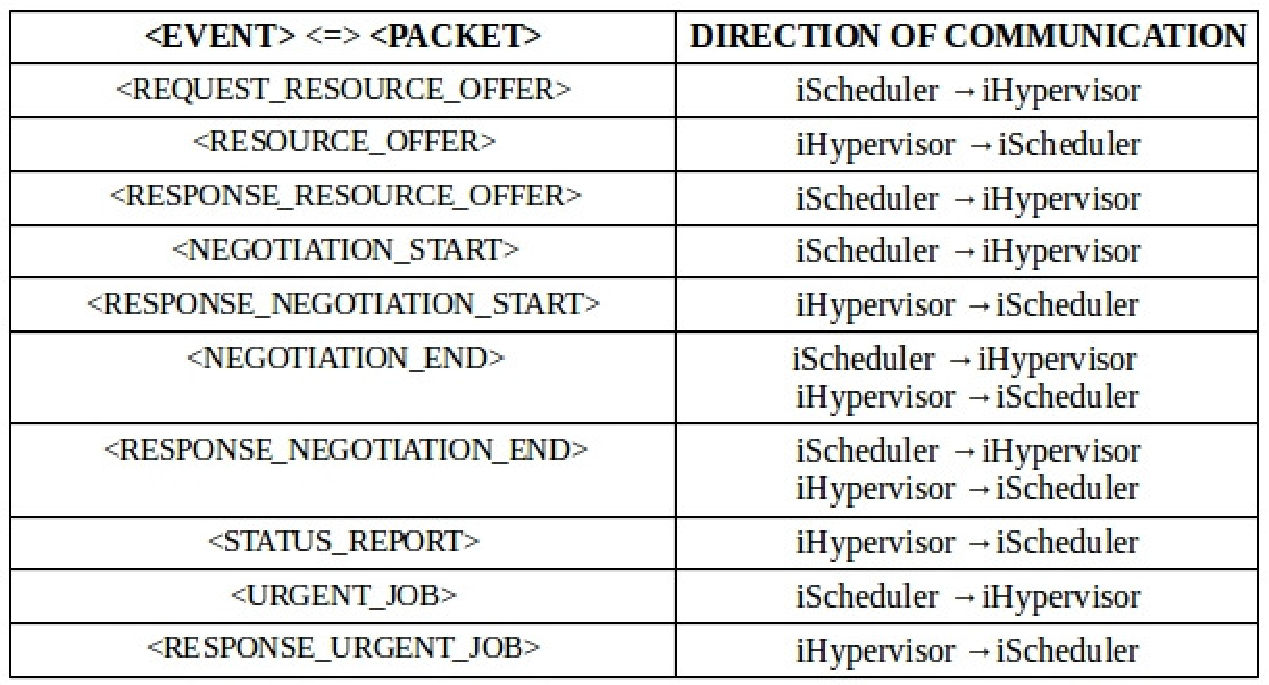
\includegraphics[width=1.0\textwidth, height=80mm]{./figures/table.pdf}
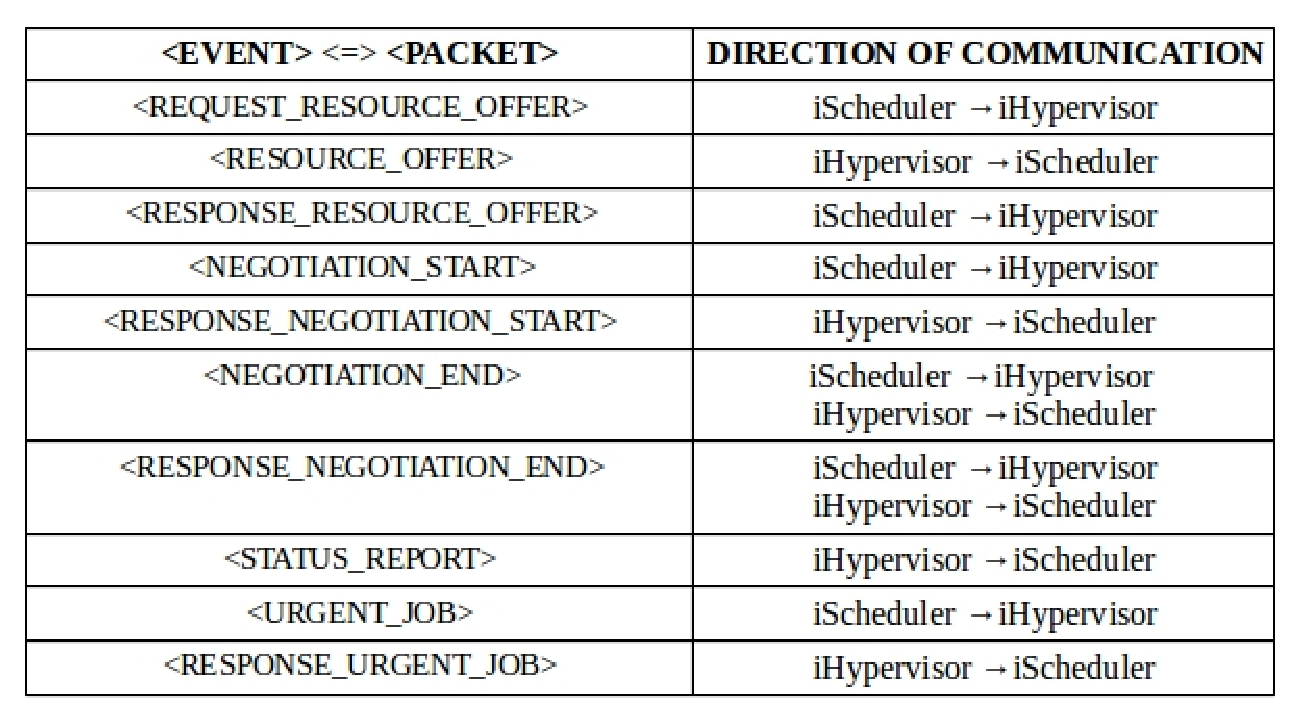
\includegraphics[width=1.0\textwidth, height=80mm]{./figures/table.eps}
\caption{Message Types}
\label{fig:8}
\end{figure}

\textbf{Communication Phases}
\begin{itemize}
\item \textbf{\textit{Protocol Initialization:}} This phase basically establishes the initial environment between the communicating parties (iScheduler and iHypervisor) for proper communication later on. Successful initialization of this phase prepares both the parties to start negotiating based on the negotiation protocol described in the following points. During this protocol initialization various parameters such as protocl version, maximum attempts for negotiation, timer intervals and several others could be exchanged to set up the internal data structures and configuration tables for both the communicating parties. This protocol is a bi-directional communication.
\item \textbf{\textit{Protocol Finalization:}} This phases signals the end of communication between iHypervisor and iScheduler using negotiation protocol. It leads to a safe termination of this communication followed by the release of any internal data structures allocated earlier along with configuration parameters. This results in consistent behaviour of both the communicating parties which can then proceed to safely terminate and exit. This protocol is a bi-directional communication.
\item \textbf{\textit{Negotiation:}} This is the most important phase in this whole approach to support invasive computing as discussed in the previous chapter. It is the phase during which both iHypervisor and iScheduler are negotiating with each other till they reach an agreement. If they do not then they continue till a certain limit to the number of negotiating attempts are reached after which both of them just agree in their final attempt closing the current negotiation. After this a new transaction of negotiation begins.
\item \textbf{\textit{Feedback:}} This concerns the periodic feedback sent by the iHypervisor to the iScheduler containing useful information such as the job states, latest snapshot of the resources in the invasic partition and many other statistical measures not limited to system utilization, job throughput, waiting times of jobs to help and influence the iScheduler in its decision making for scheduling jobs during its future transactions of negotiation. This protocol is a uni-directional communication.
\item \textbf{\textit{Urgent Jobs:}} This protocol concerns the support for urgent jobs. At any given point of time a cluster or supercomputing center may want to support very high priority jobs immediately without any further delay. By introducing support for invasive computing, it makes it all the more feasible to help run these urgent jobs immediately by either shrinking the resources of other jobs or suspending/Killing them.
\end{itemize}

\textbf{\textit{Separation of Concerns: }}In this thesis, The idea of separating the batch and runtime scheduling components of a Job Scheduler is explored. 

\subsection{Batch Scheduler}
Today almost all resource management systems fall into the category of queuing systems. Several queues with different limits on the number of requested resources and the duration exist for the submission of resource requests. Jobs within a queue are ordered according to a scheduling policy, e. g. FCFS (first come, first serve). Queues might be activated only for specific times (e. g. prime time, non prime time, or weekend). The task of a queuing system is to assign free resources to waiting requests. The highest prioritized request is always the queue head. If it is possible to start more than one queue head, further criteria like queue priority or best fit (e. g. leaving less resources idle) are used to select a request. There might also exist a high priority queue whose jobs are preferred at any time. If not enough resources are available to start any of the queue heads, the system waits until enough resources become available. These idle resources may be utilized with less prioritized requests by backfilling mechanisms.
\subsection{Distributed Run Time Scheduler}
\subsection{MPI Process Manager}


\section{Negotiation Protocol}
\subsection{Protocol Sequence Diagrams}
\vspace{-0.15in}
\begin{figure}[!htbp]
%\begin{figure}[H]
\centering
%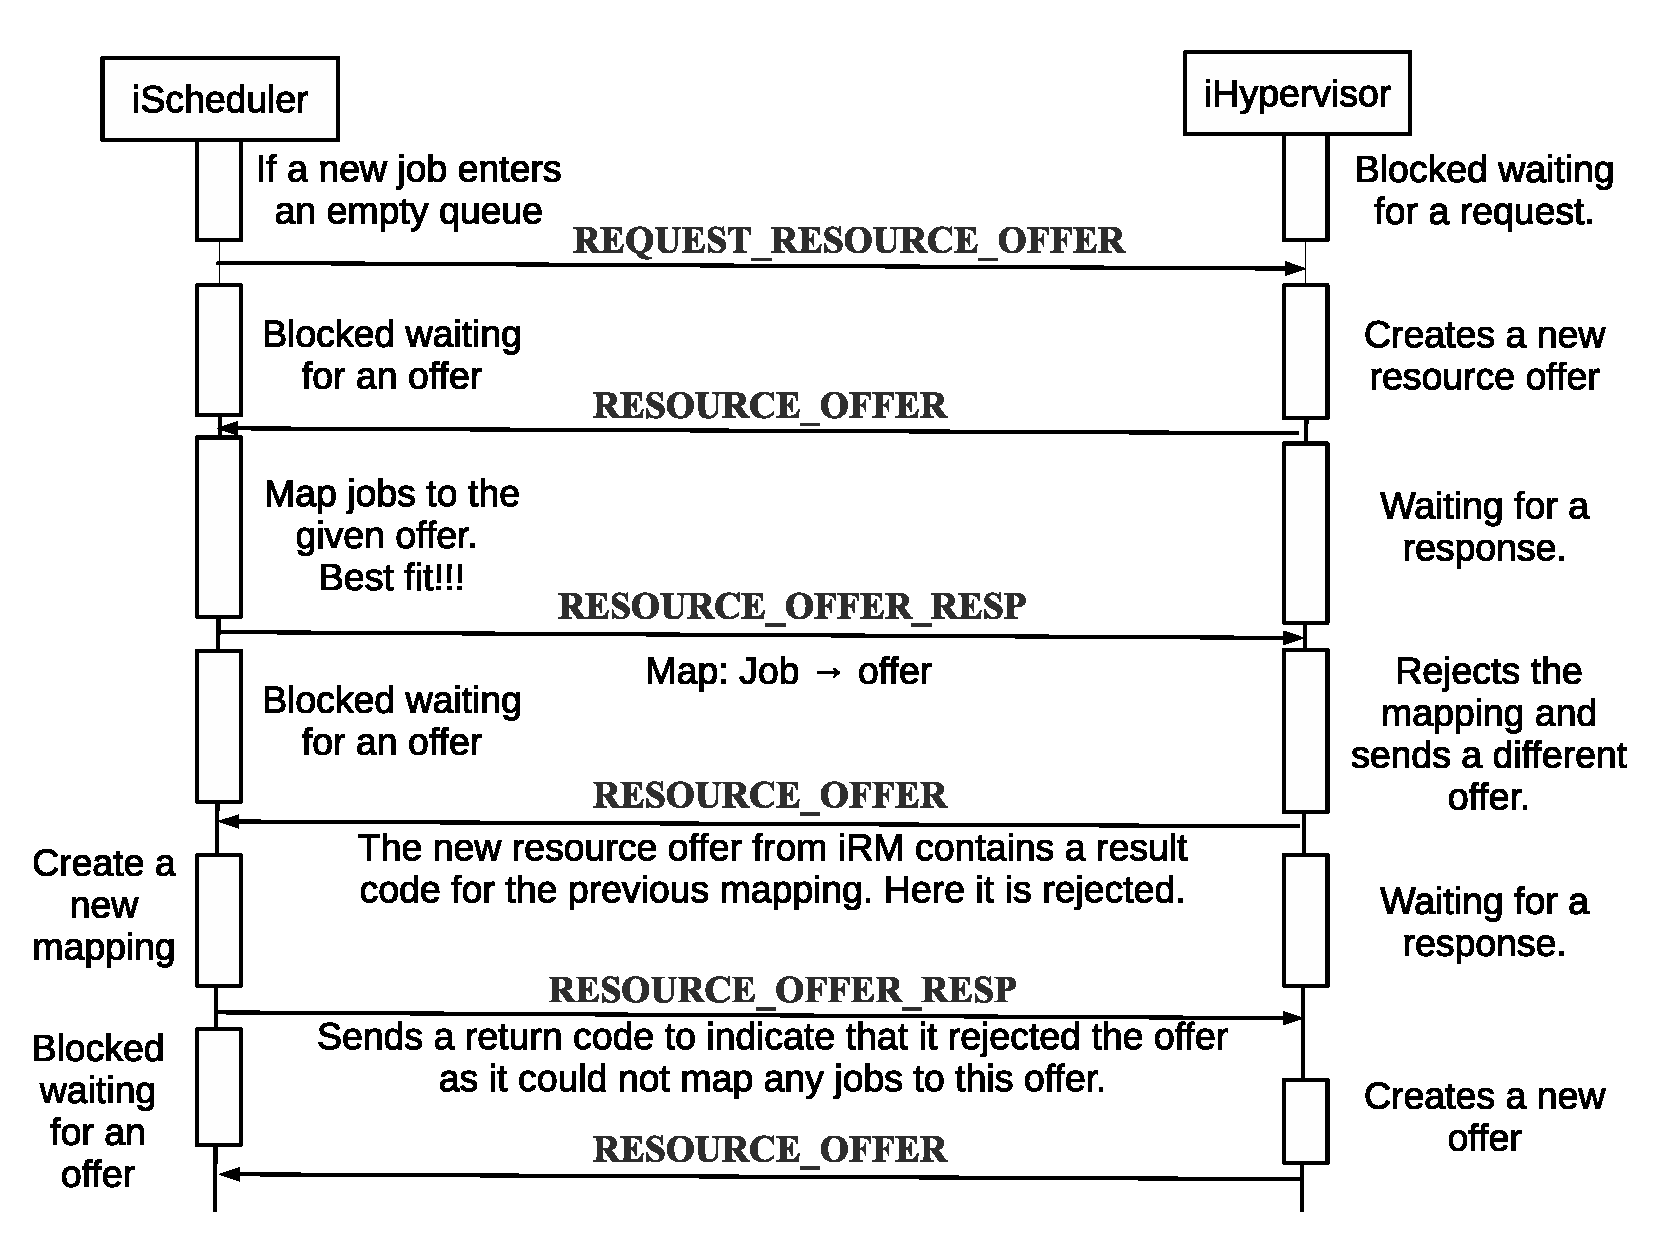
\includegraphics[width=1.0\textwidth, height=100mm]{./figures/figures.pdf}
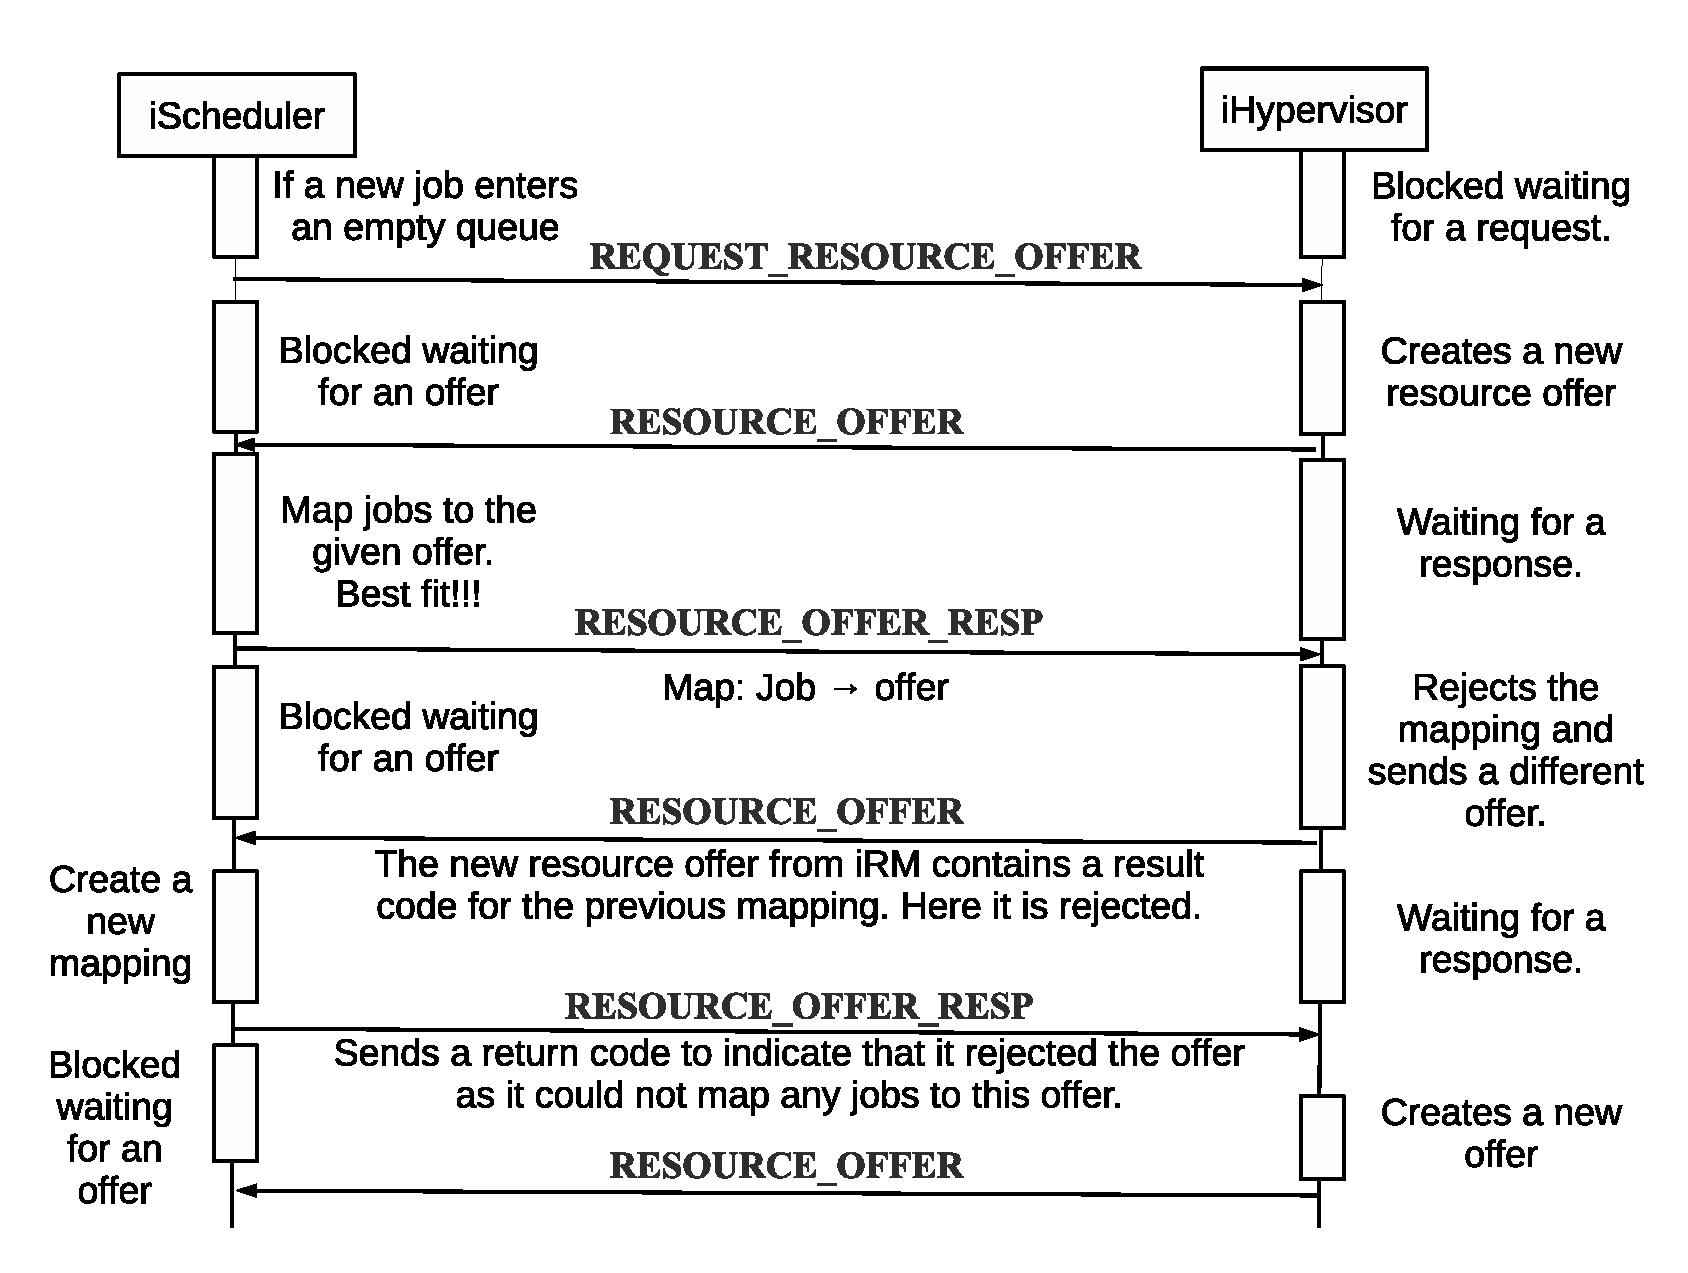
\includegraphics[width=1.0\textwidth, height=100mm]{./figures/figures.eps}
\caption{Scenario 1}
\begin{itemize}
\item Above diagram illustrates a scenario where both iScheduler and iHpervisor are negotiating with each other. The scenario is continued in the next page. \ref{fig:Seq2} illustrates another scenario where negotiations may stop when job queue becomes empty and iHypevisor then will wait for a request from iScheduler for a resource offer that will happen when new jobs arrive.
\item iScheduler makes scheduling decisions at a coarser level of granularity which is nodes whereas iHypervisor does at the granularity of cores and sockets. Both will negotiate with each other till they reach an agreement.
\item It is an event based scheduling which means iScheduler makes a scheduling decision only when it is triggered by receiving a resource offer from iHypervisor. It is only at the start when there are no jobs in the queue and during the operations when the queue may become empty that the iScheduler will have to explicitly send a request message to iHypervisor for a resource offer otherwise at all other times scheduling is event based.
\end{itemize}
\label{fig:Seq1}
\end{figure}
\vspace{-0.25in}
\begin{figure}[!htbp]
\centering
%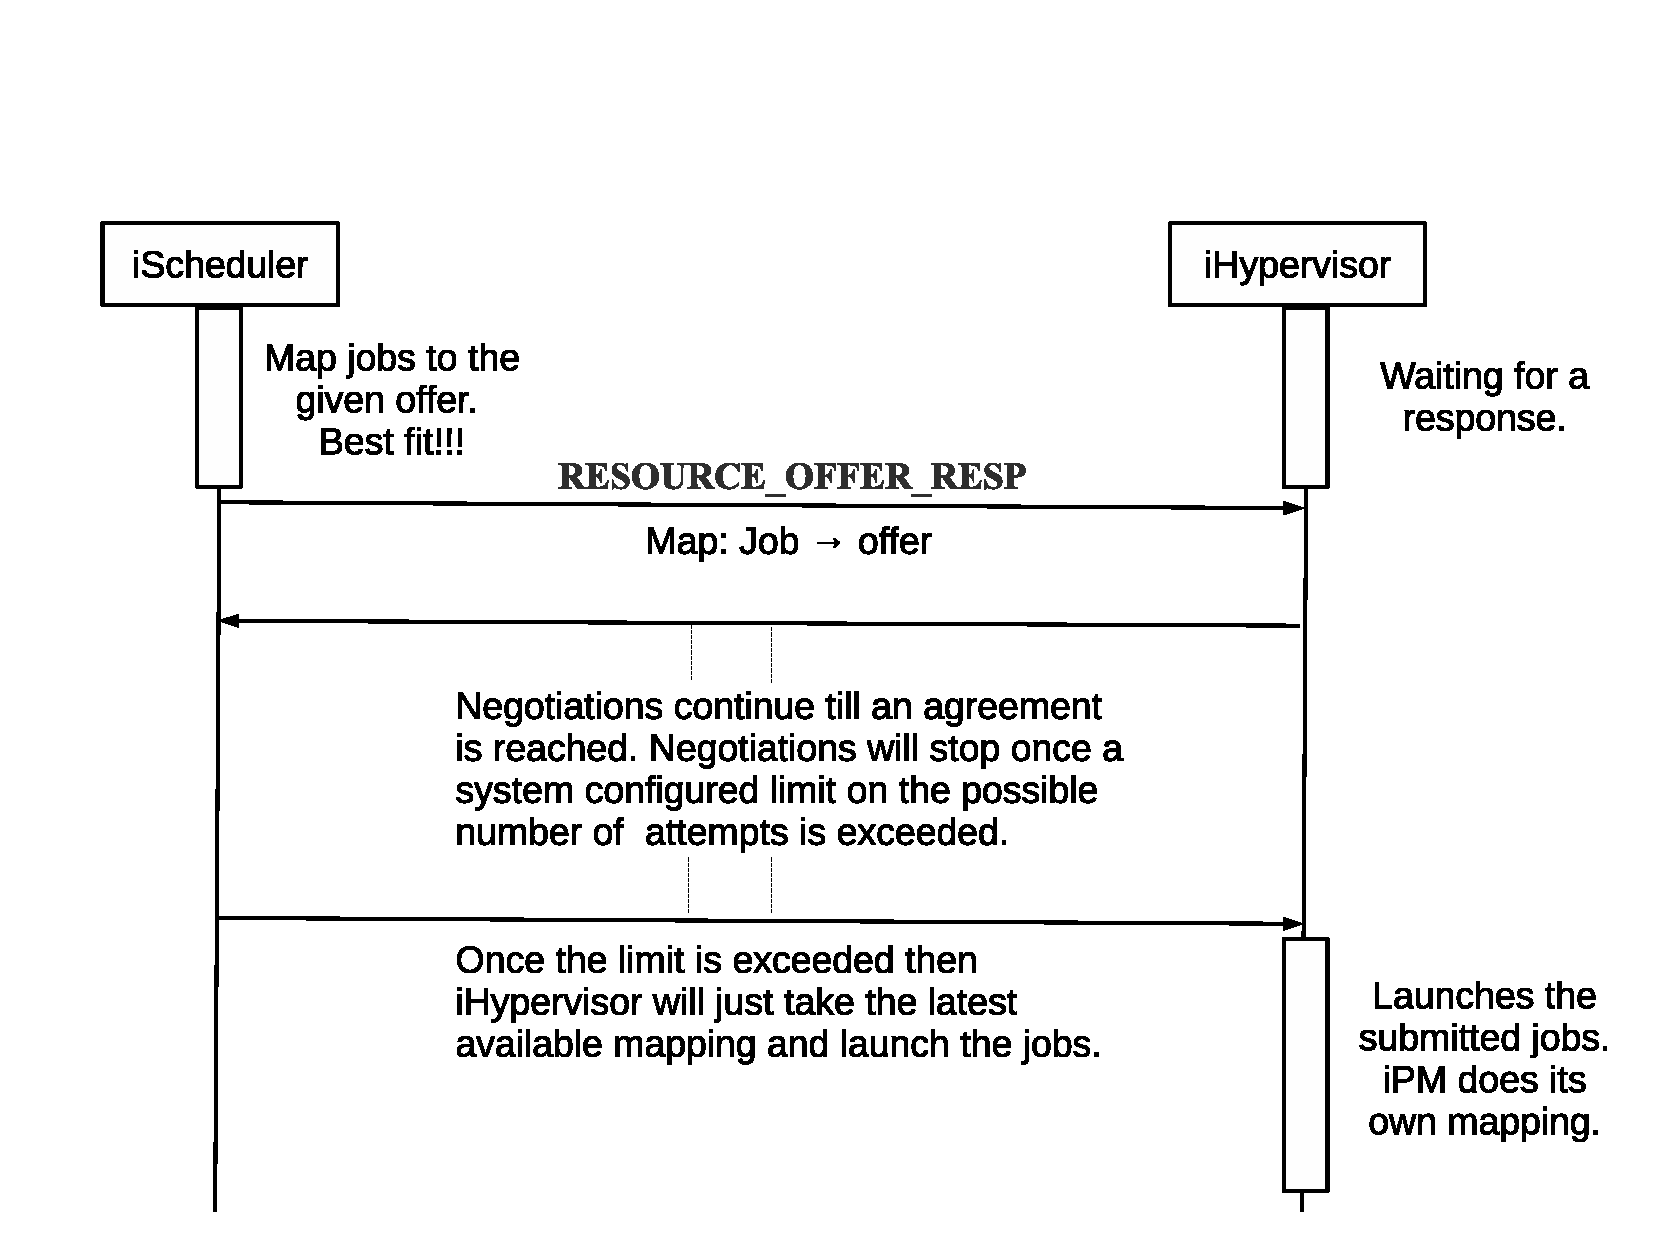
\includegraphics[width=0.9\textwidth, height=100mm]{./figures/figures1.pdf}
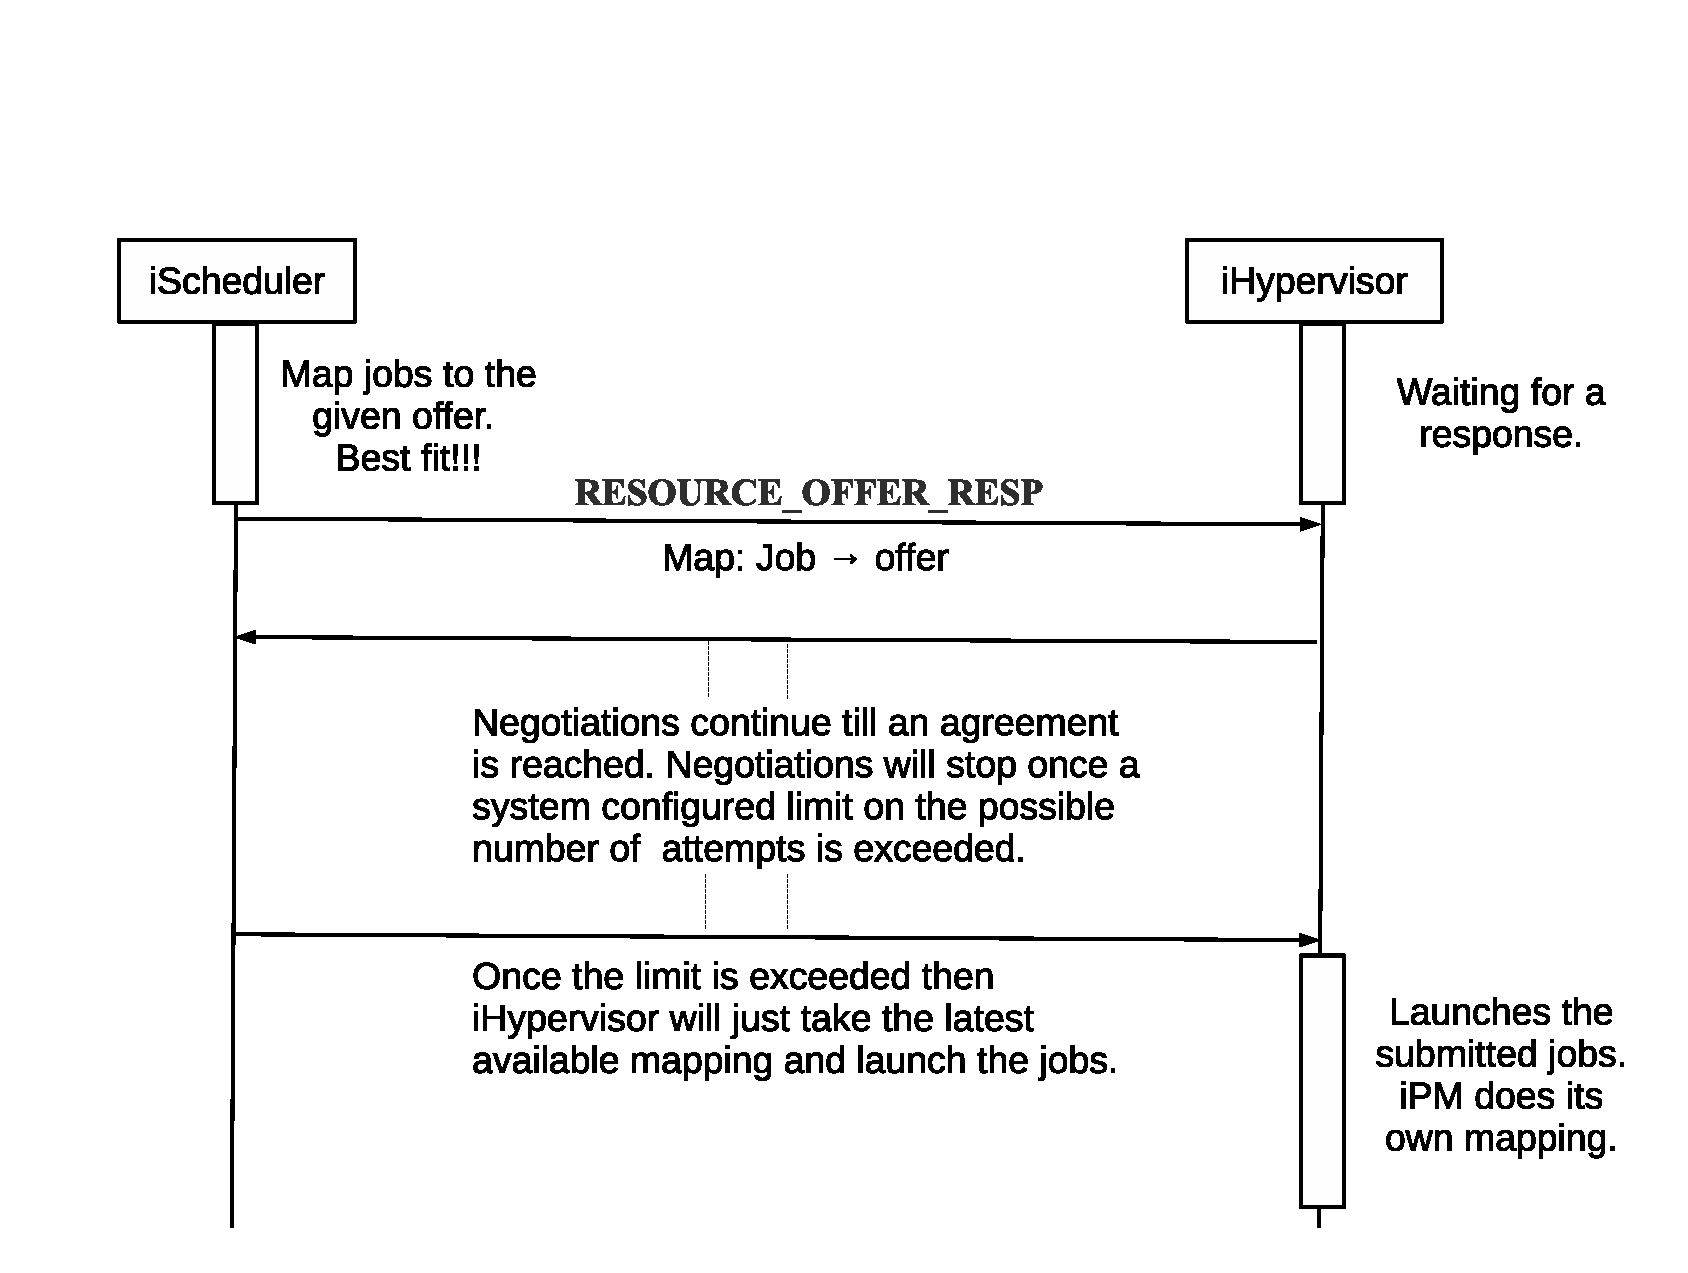
\includegraphics[width=0.9\textwidth, height=100mm]{./figures/figures1.eps}
\caption{Scenario 1 contd.}
\label{fig:Seq1}
\vspace{0.25in}
%\end{figure}
%\begin{figure}[b]
\centering
%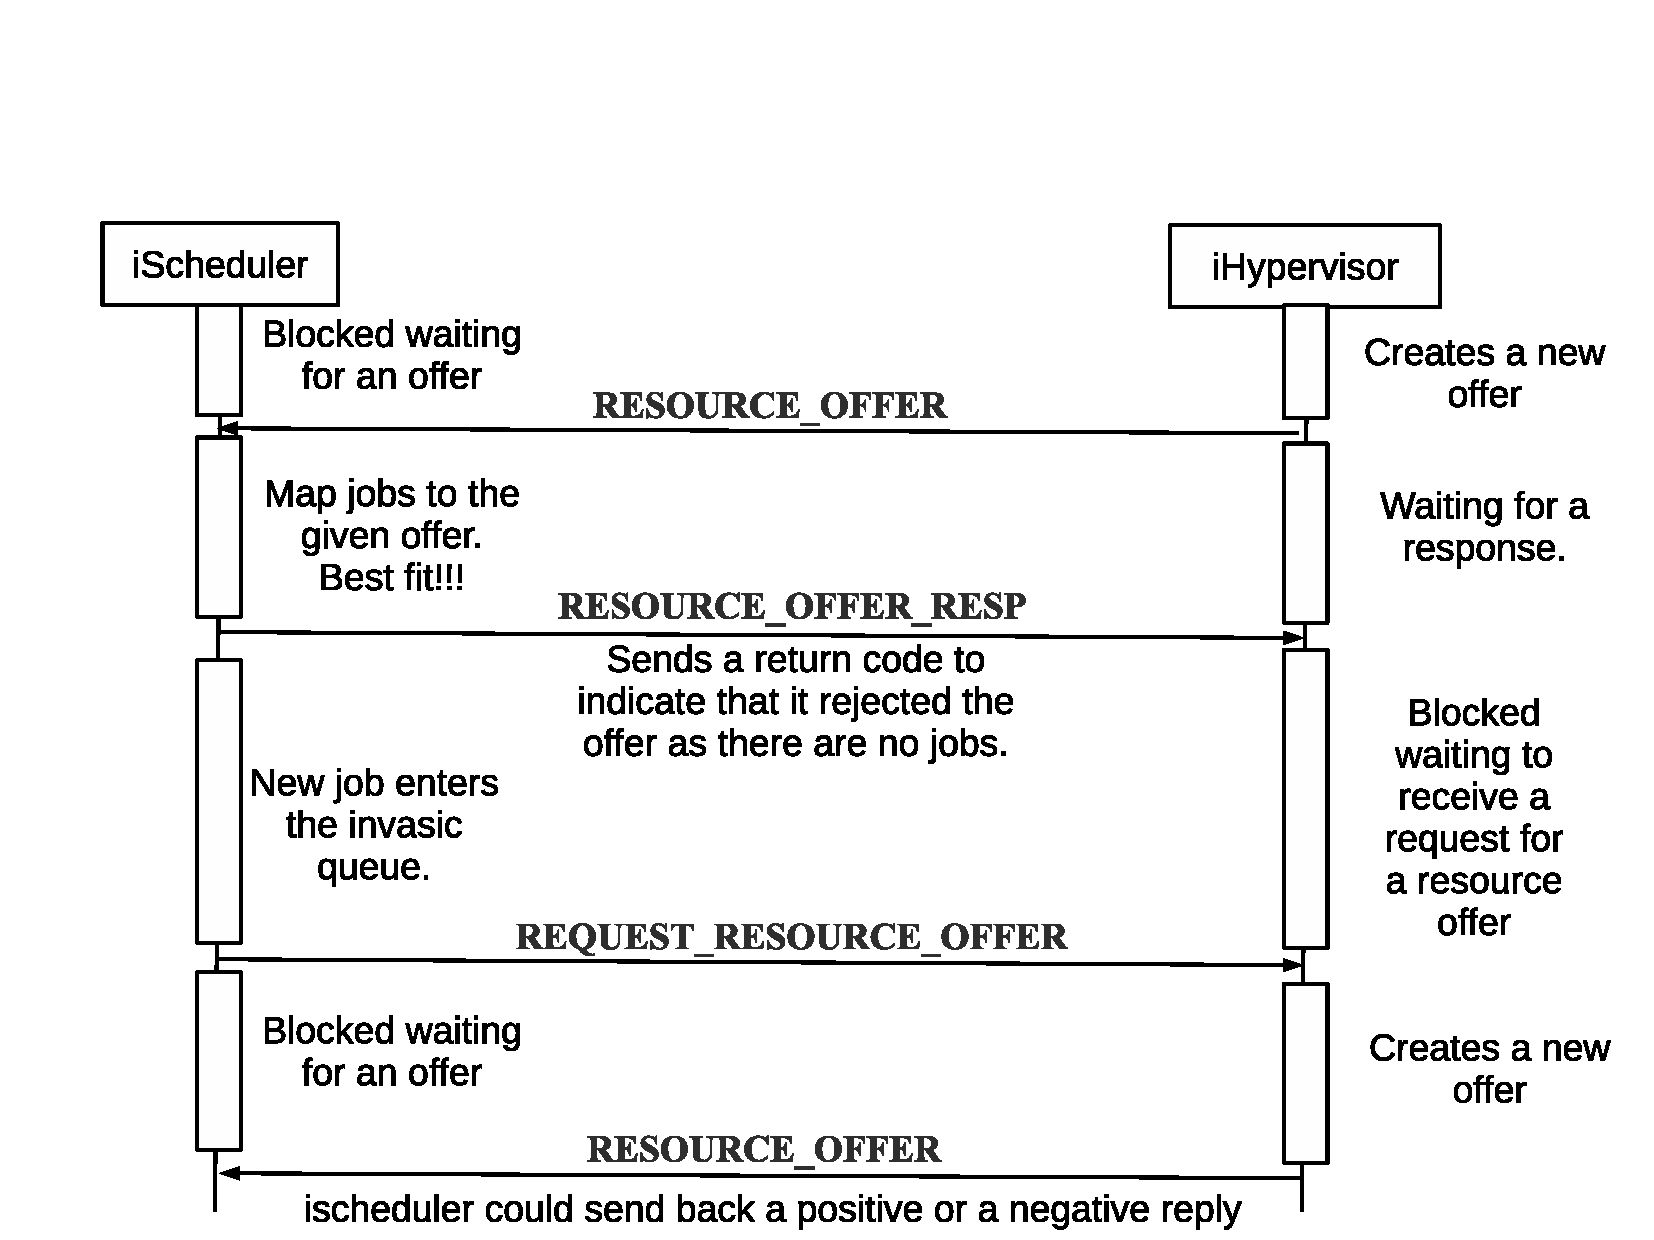
\includegraphics[width=0.9\textwidth, height=100mm]{./figures/figures2.pdf}
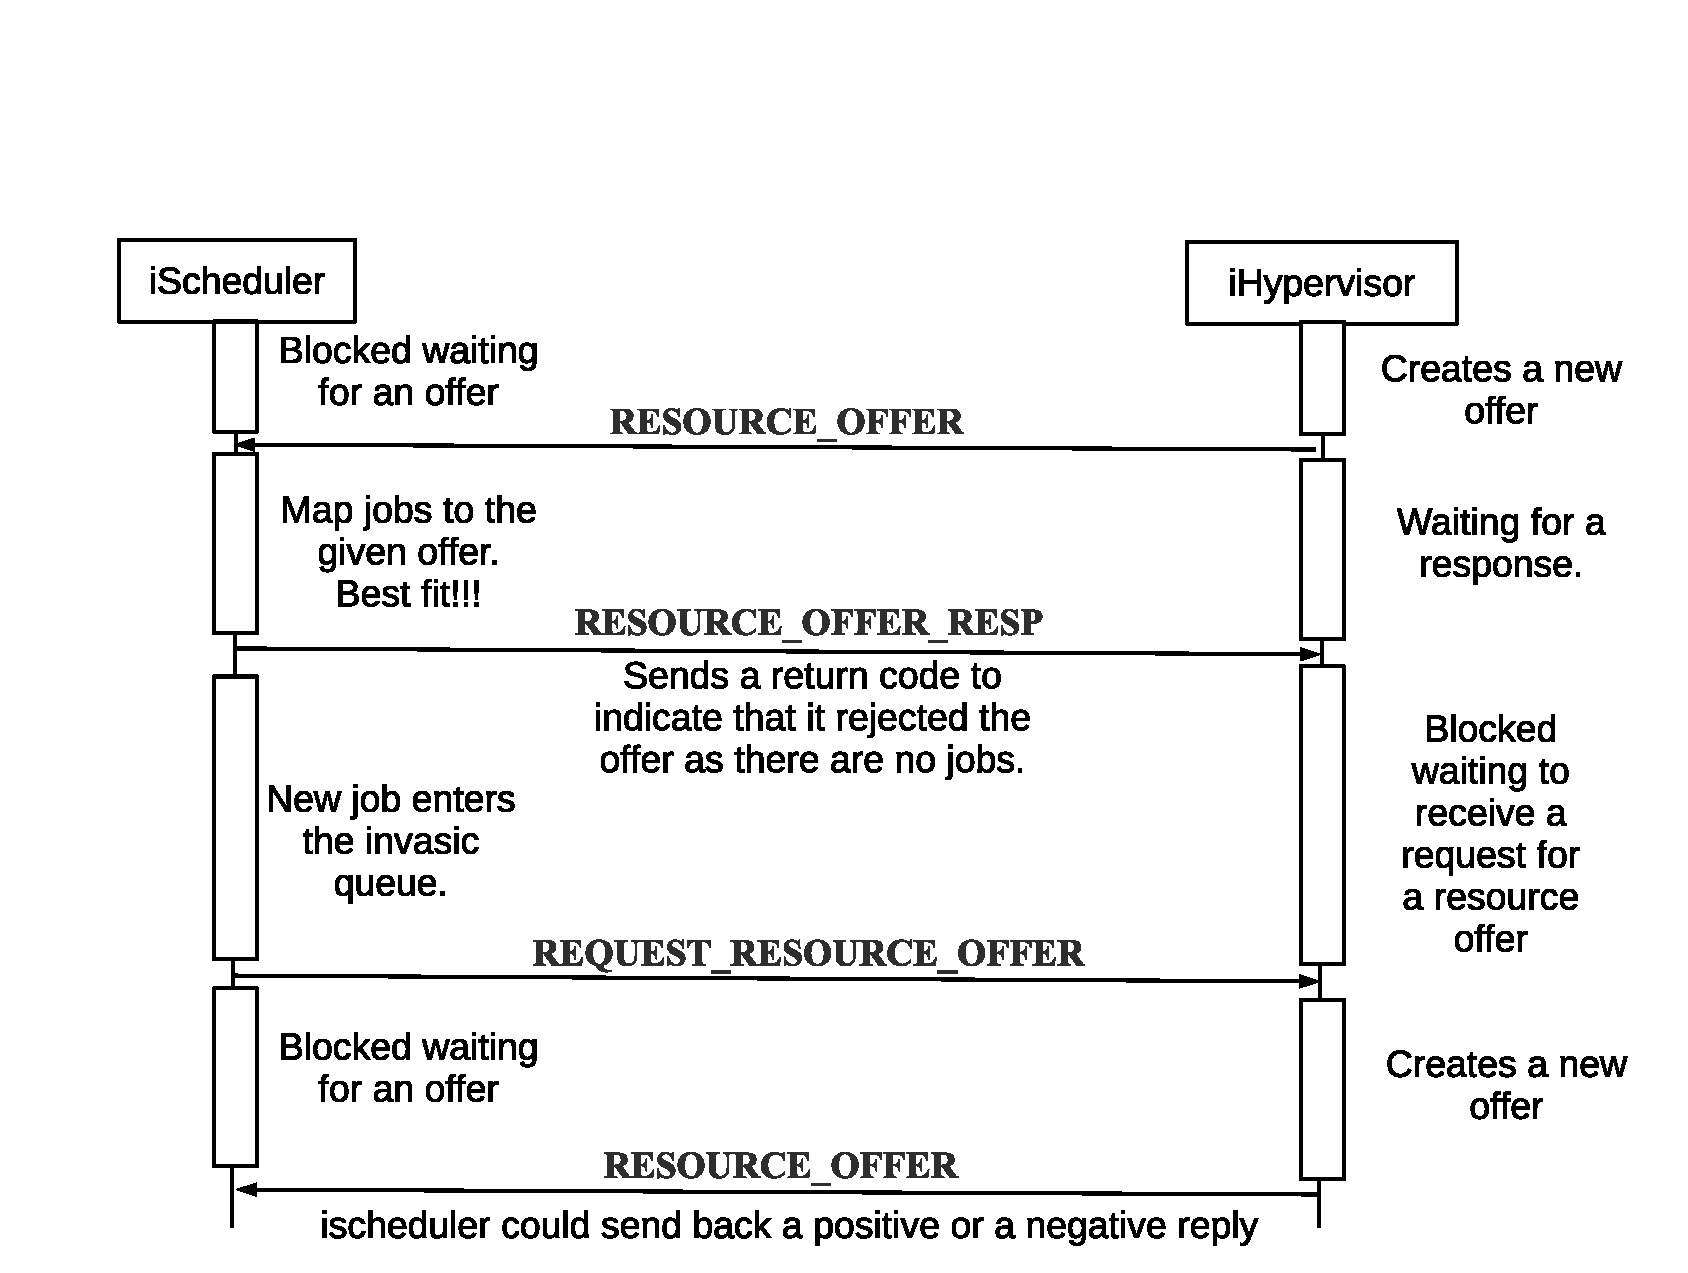
\includegraphics[width=0.9\textwidth, height=100mm]{./figures/figures2.eps}
\caption{Scenario 2}
\label{fig:Seq2}
\end{figure}
\subsection{State Machine Diagrams}
This section focuses on iScheduler and a thread iRM\_AGENT that it spawns which is the one responsible for all the communication with the iHypervisor including spawning other agent threads for handling feedbacks and urgent jobs.
\vspace{10mm}
\begin{figure}[h]
\centering
%\includegraphics[width=1.0\textwidth, height=150mm]{./figures/"iRM Agent".pdf}
\includegraphics[width=1.0\textwidth, height=150mm]{./figures/"iRM Agent".eps}
\caption{iRM Agent}
\label{fig:Init}
\end{figure}
\begin{itemize}
\item Above diagram and the ones in the following pages illustrate state machine diagrams for few of the communication phases described earlier starting first with a general diagram of how the mulithreaded component iRM agent inside iScheduler starts up and shuts down.
\end{itemize}
\vspace{-20mm}
\begin{figure}[h]
\centering
%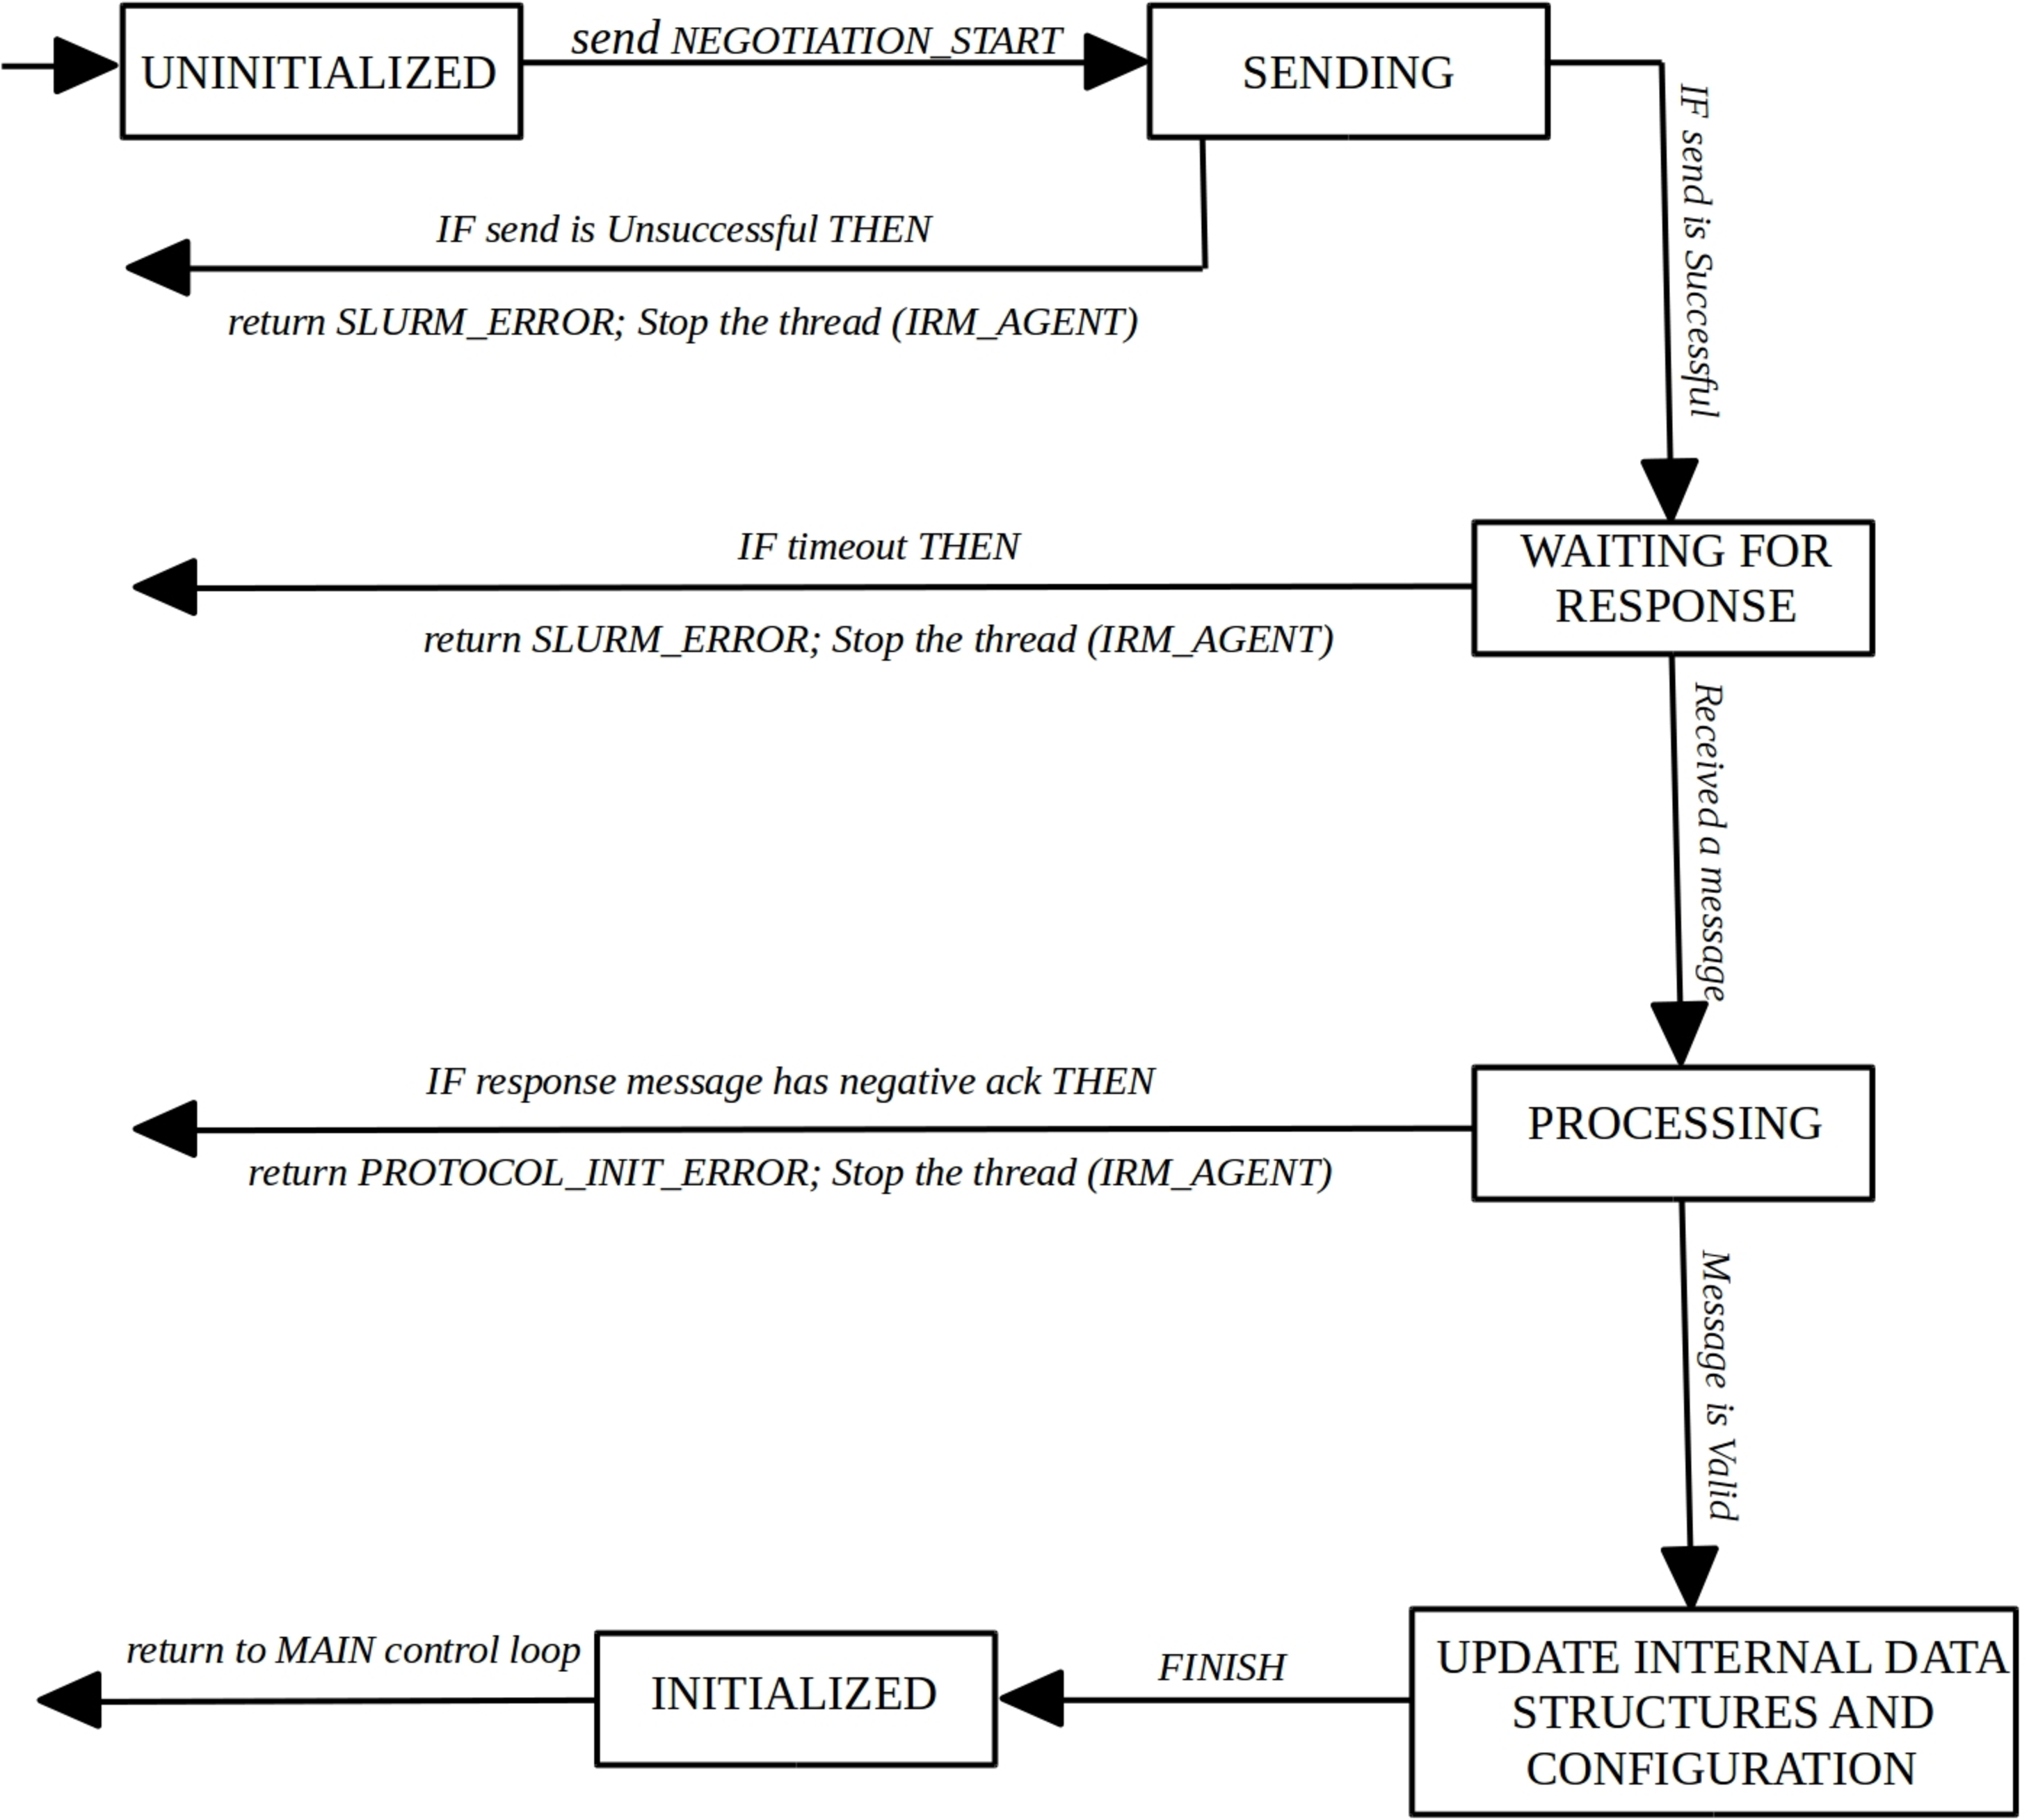
\includegraphics[width=0.9\textwidth, height=90mm]{./figures/Init.pdf}
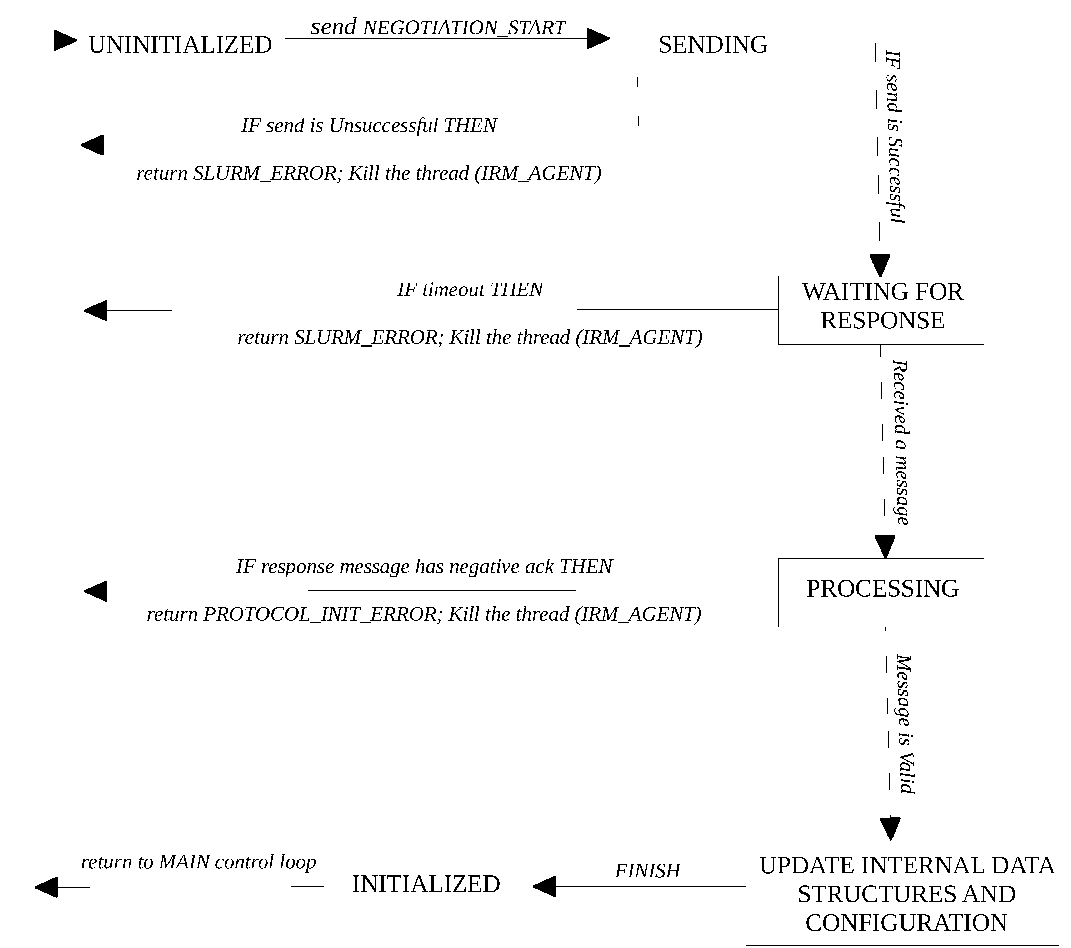
\includegraphics[width=0.9\textwidth, height=90mm]{./figures/Init.eps}
\caption{Protocol Initialization}
\label{fig:Init}
\end{figure}
\vspace{5mm}
\begin{figure}[h]
\centering
%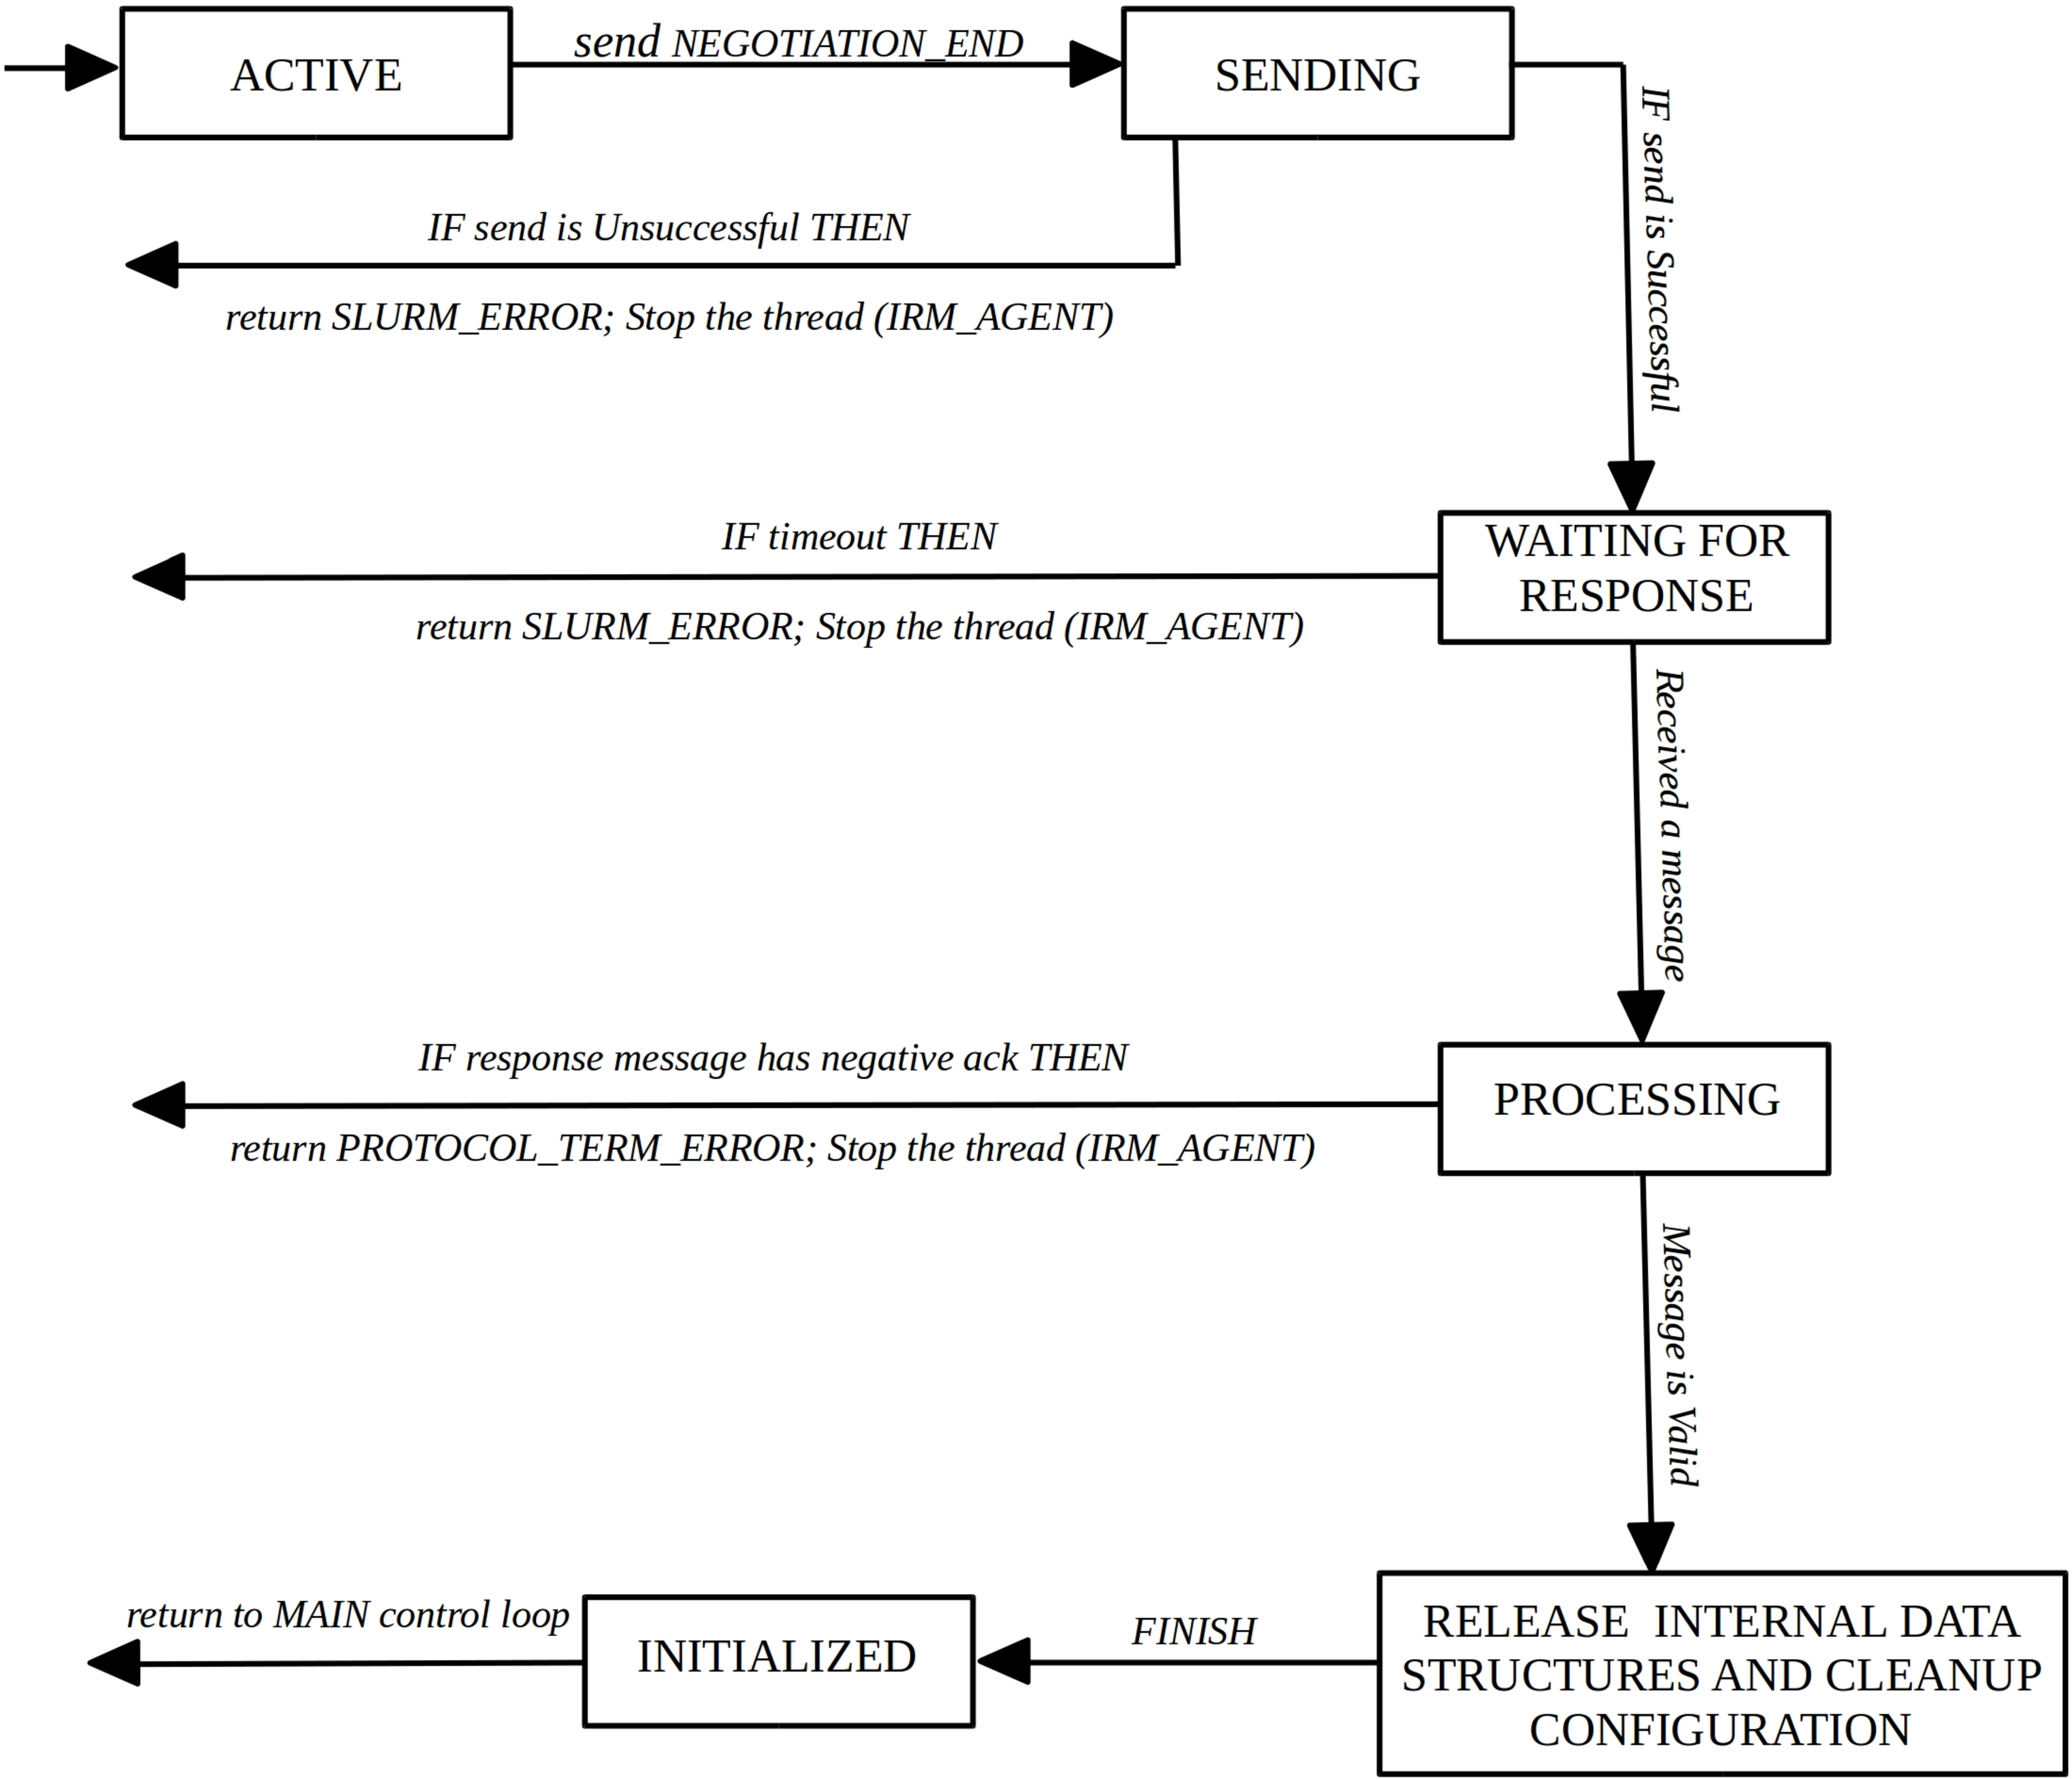
\includegraphics[width=0.9\textwidth, height=90mm]{./figures/Term.pdf}
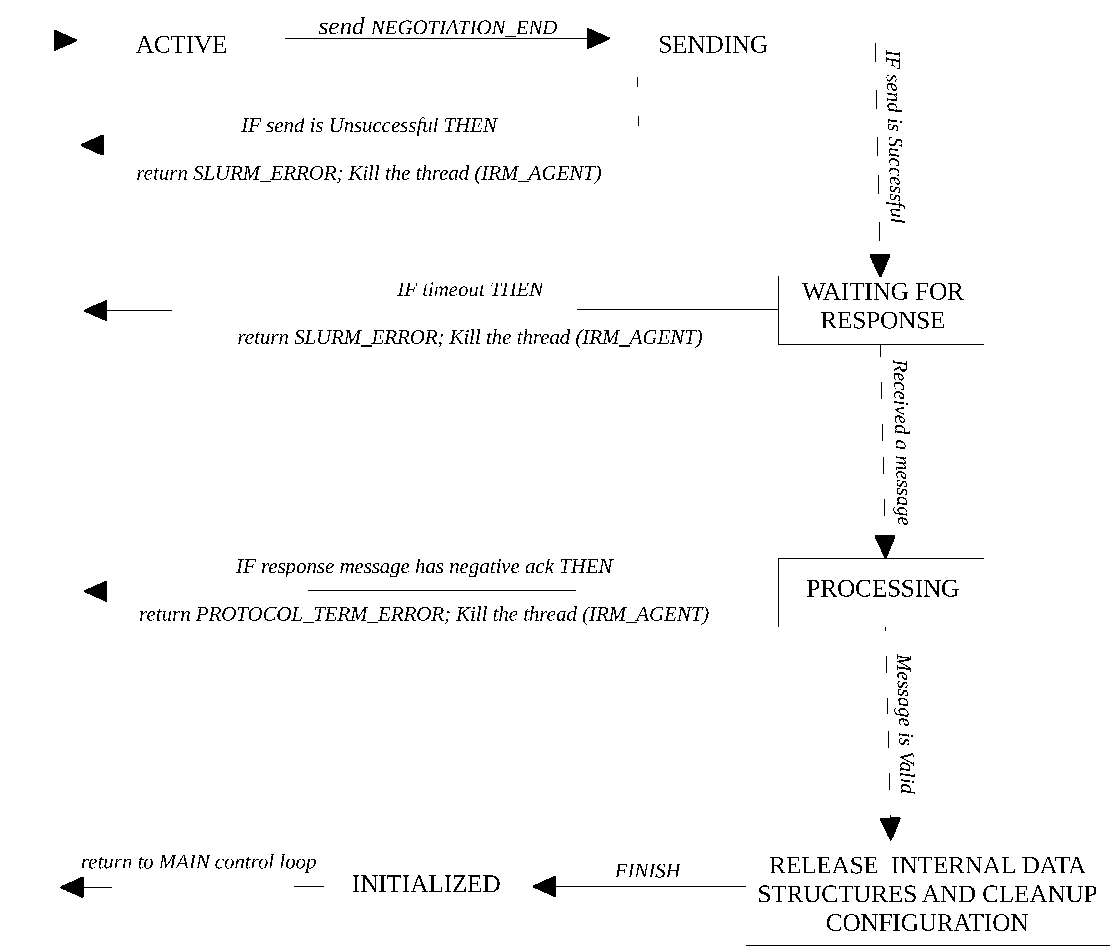
\includegraphics[width=0.9\textwidth, height=90mm]{./figures/Term.eps}
\caption{Protocol Termination}
\label{fig:Term}
\end{figure}
\clearpage
\begin{figure}[h]
\centering
%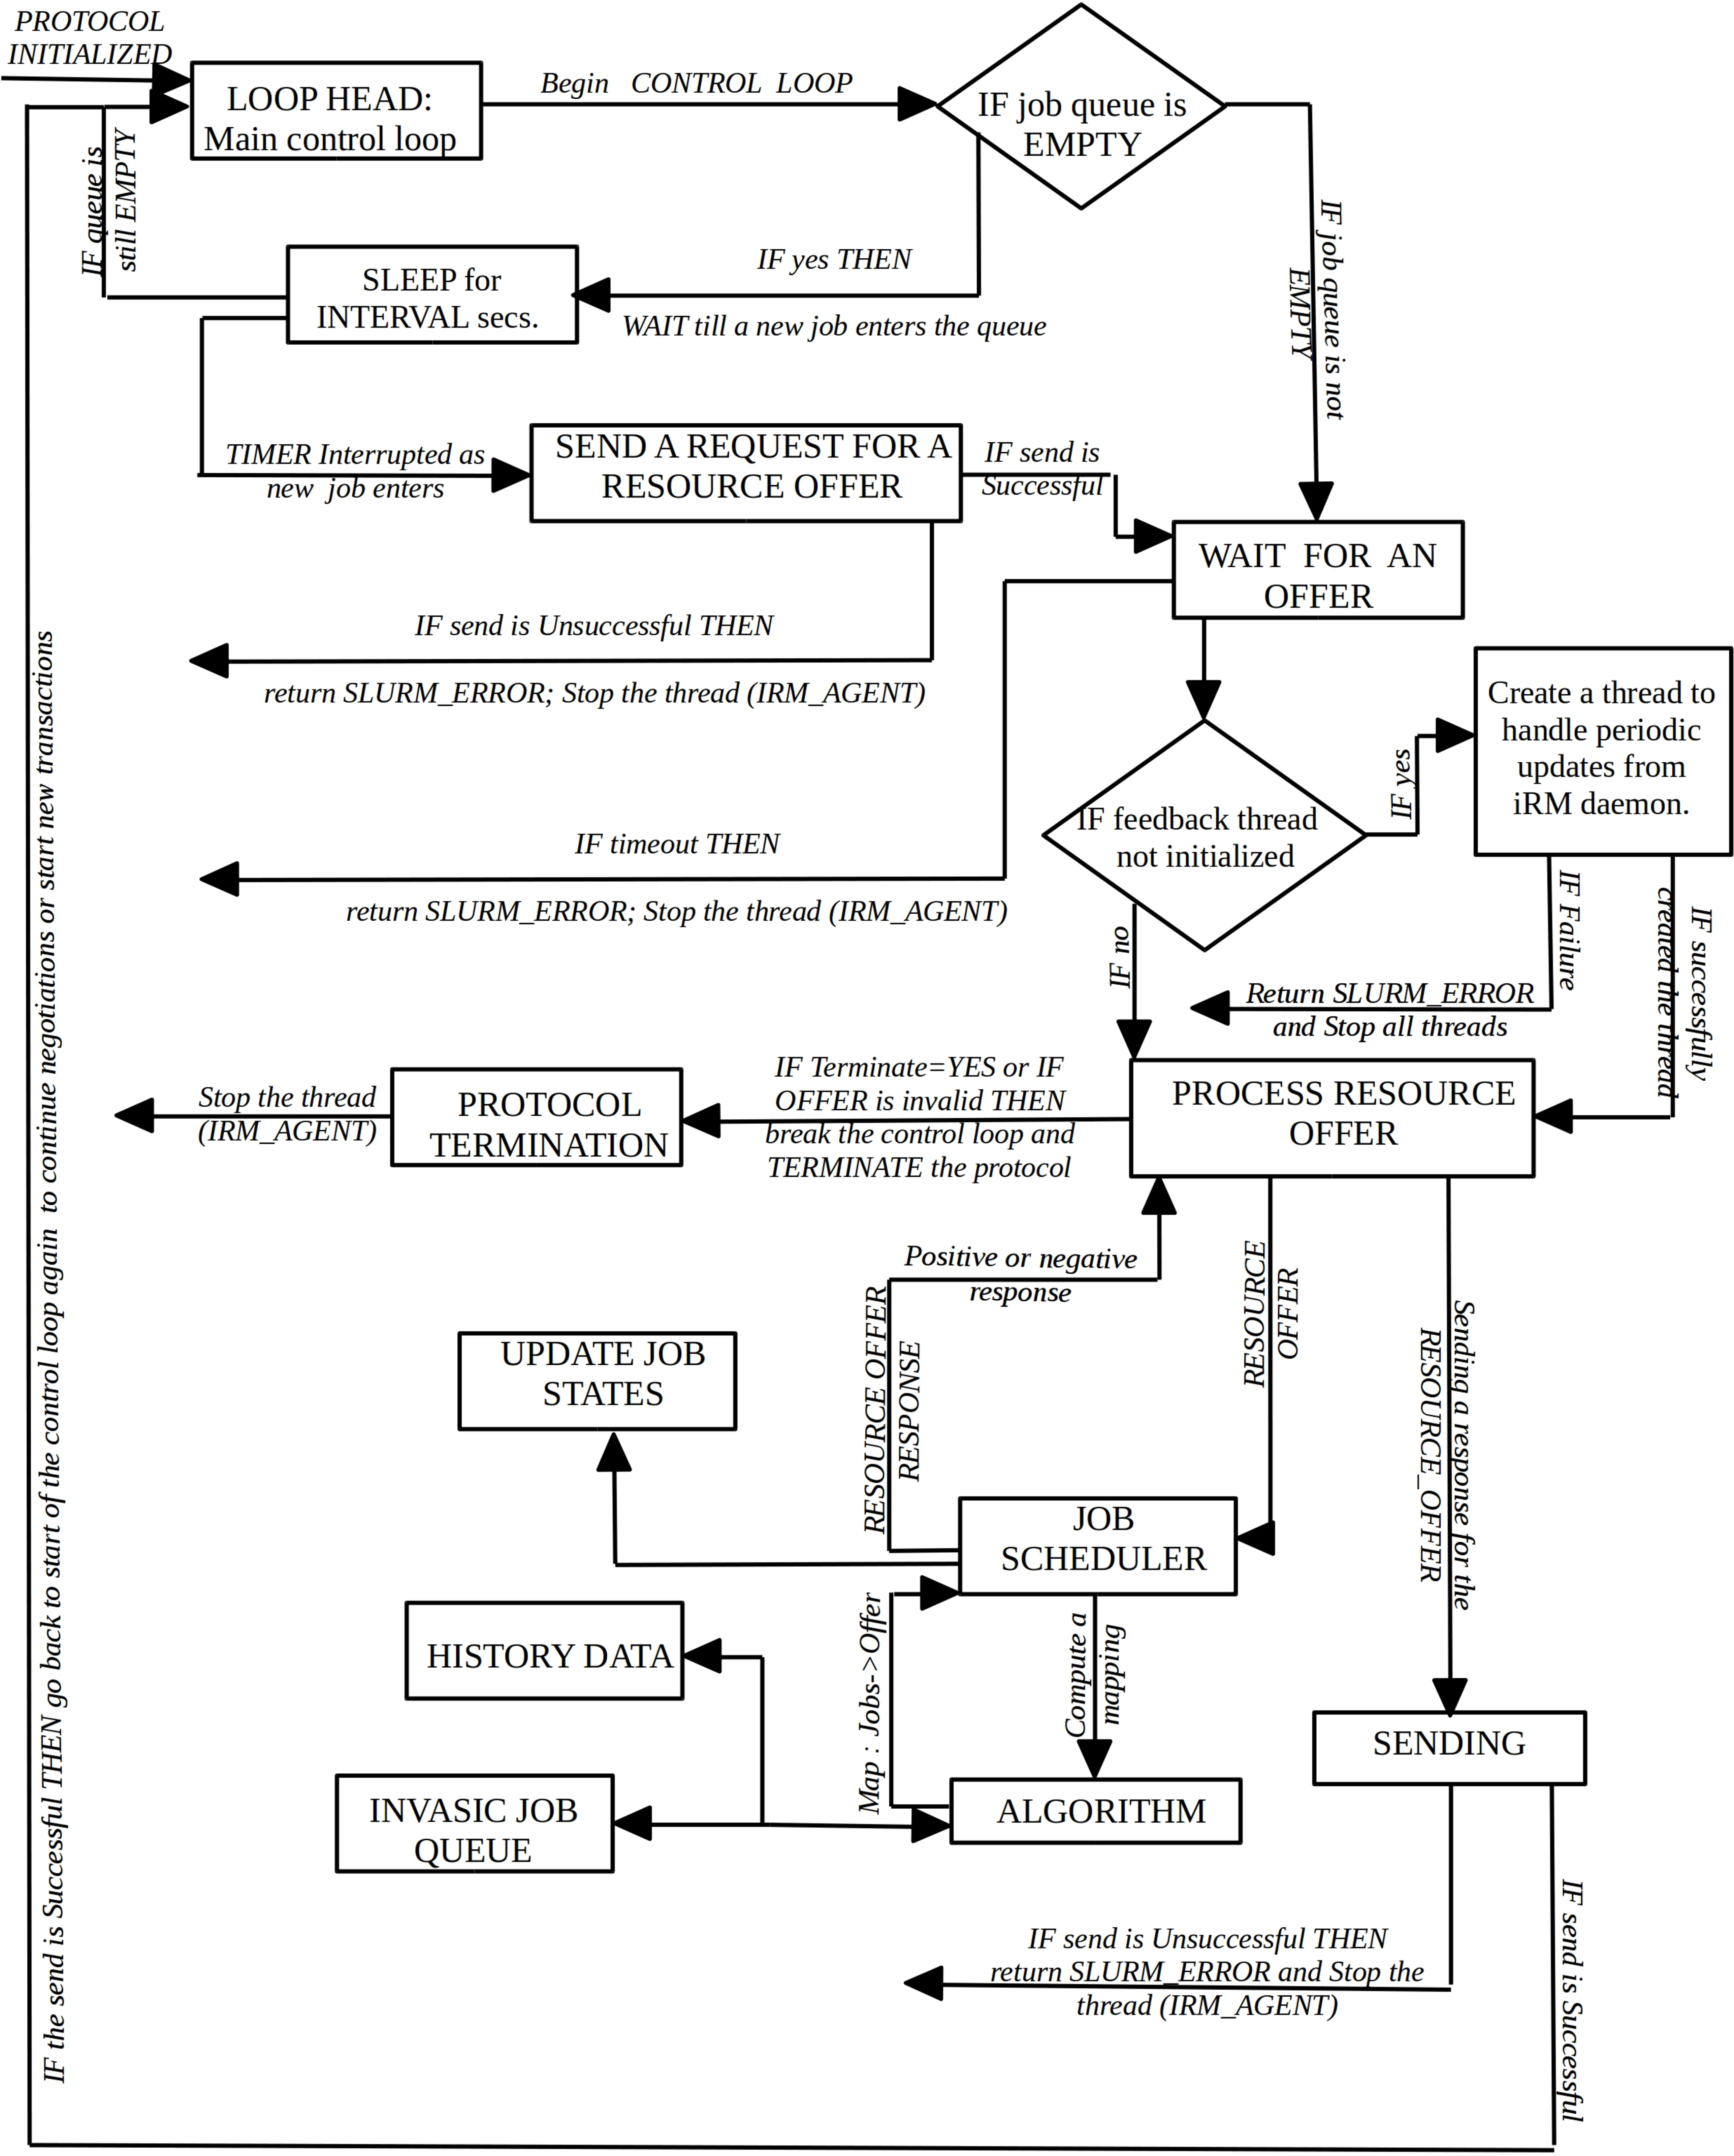
\includegraphics[width=1.0\textwidth, height=210mm]{./figures/Negotiation.pdf}
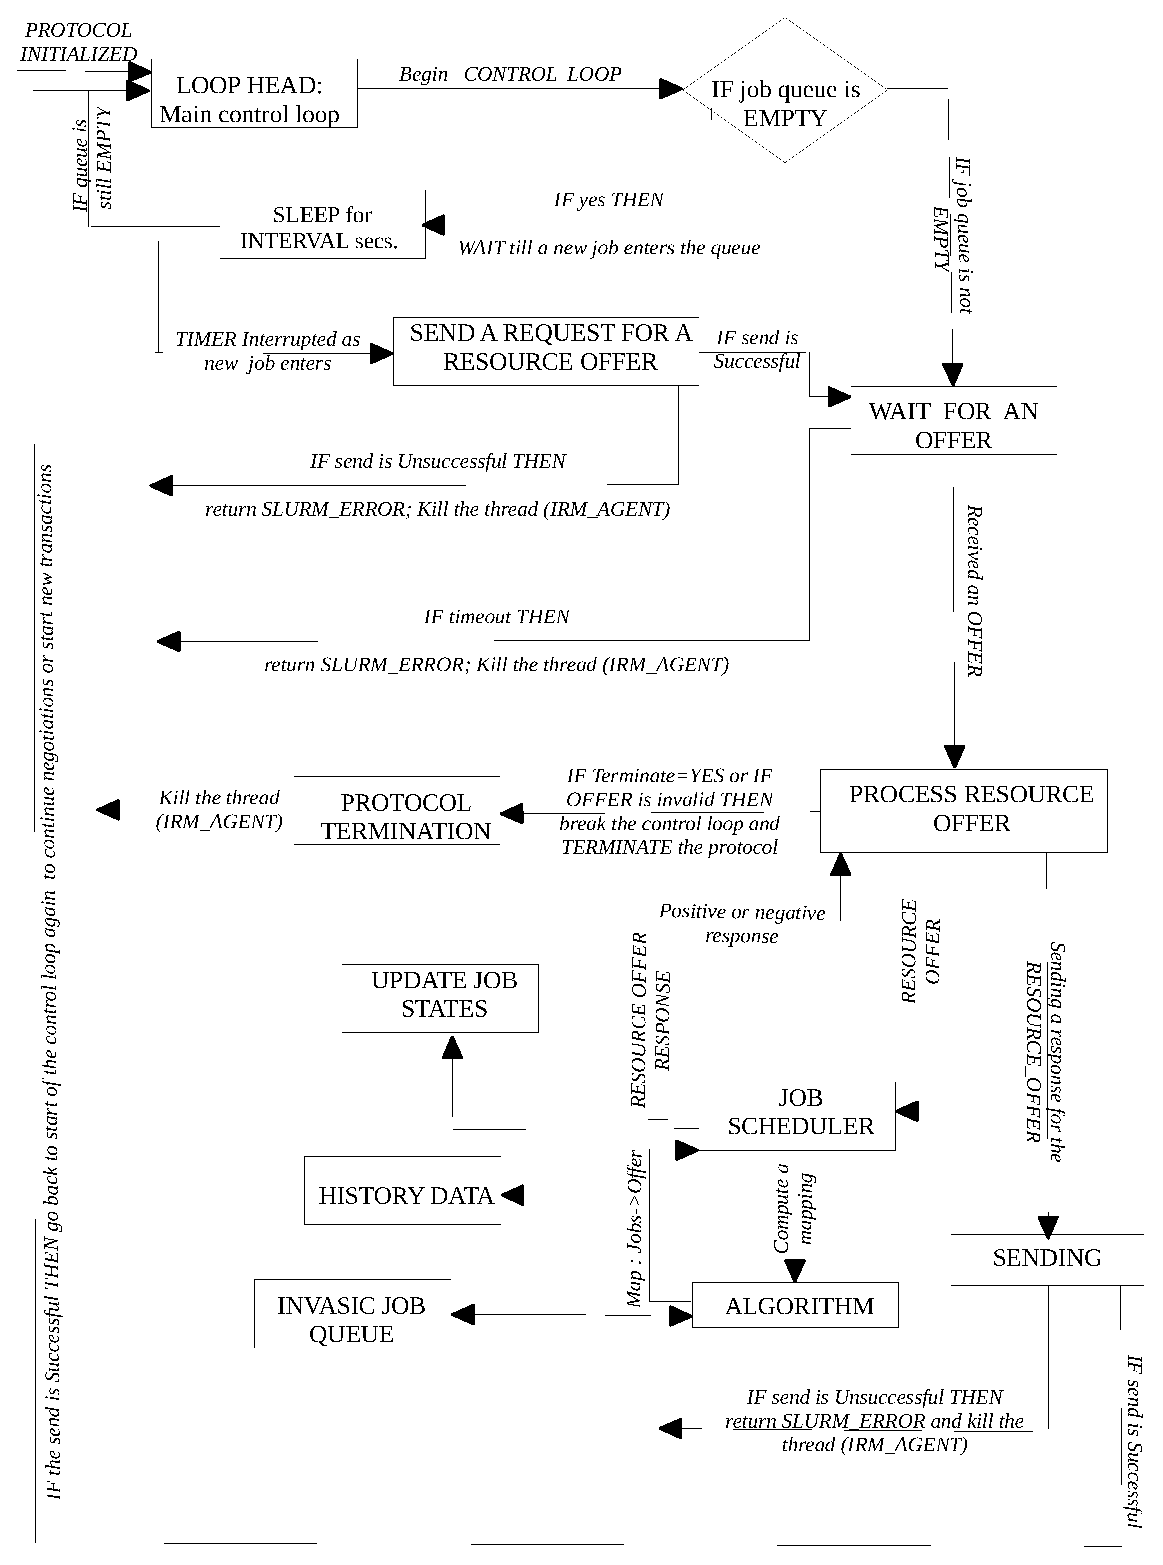
\includegraphics[width=1.0\textwidth, height=210mm]{./figures/Negotiation.eps}
\caption{Negotiation}
\label{fig:Neg}
\end{figure}
\clearpage

\section{Invasive Jobs}

\chapter{Design}
In this section, we will describe the internal details of the components in the architecture specifically on how the scheduling algorithms work in order to realize the negotiation, the meaning of job mappings, resource offers and feedback reports. 
\label{chapter:ischeduler}
\section{Entities}
A design entity is an element(component) of a design that is structurally and functionally distinct from other elements and that is separately named and referenced. They result from the decomposition of the software system requirements. The objective is to divide the system into separate components that can be considered, implemented, changed, and tested with minimal effect on other entities. Examples of design entities are: \textbf{\textit{protocol, application layer, state machine, data model, object, task, sub-systems, modules}} etc.\\ \\
\textbf{Job Mappings}\\
A job mapping is basically a job and its allocated set of resources. A forward job record is a job mapping and other related job details important for its launch. A list of such forward job records are sent by the batch scheduler in response to receiving a resource offer from the runtime scheduler.\\
%\vspace{-0.5in}
%\begin{center}
\begin{equation*}
%\begin{multlined}
\begin{aligned}
&M_{i}\ \ \ \textit{:=\ \ \ Job Mapping\ \ \ :=}\ \ \ \{jobid,node count,bitmap\}\\
&Map_{i}\ \ \ \textit{:=\ \ \ Forward Job Record\ \ \ :=}\ \ \ \{M_{i},details_{i}\}\\
&Map\ \ \ \textit{:=\ \ \ {$<Map_{1}><Map_{2}>...<Map_{n}>$}}
%\end{multlined}
\end{aligned}
\end{equation*}
%\end{center}
In the above description $details_{i}$ refers to the details of any $i^{th}$ job such as \textit{constraints, priority, runtime estimate, max nodes, min nodes, job name, start time, deadline}. In these details, the constraints are specific to the purpose of negotiation and this can be related to node count that the job is requesting for, memory size, exclusive / shared resource access etc. Currently, we support only the constraints for node count. The node count constraint will again have a min and max both of which will fall within the window of max and min nodes of the job. It is using these constraints that the batch scheduler will negotiate with the runtime scheduler and with every negotiation attempt it will relax the constraints to bargain better.\\ \\
\textbf{Resource Offers}\\
A reservation is basically a job being guaranteed a set of resources for a certain period of time. A resource offer is a list of such reservations and the set of nodes which are free in the partition after the runtime scheduler has guaranteed these reservations. The runtime scheduler will send such a resource offer to the batch scheduler if it rejected its mapping or it is sending a new offer that it generated.\\
%\vspace{-0.5in}
%\begin{center}
\begin{equation*}
%\begin{multlined}
\begin{aligned}
&Resv_{i}\ \ \ \textit{:=\ \ \ Job Reservation\ \ \ :=}\ \ \ \{jobid,node count,bitmap,start time,end time\}\\
&IdleNodes\ \ \ \textit{:=\ \ \ Residual Nodes\ \ \ :=}\ \ \ \{bitmap\}\\
&Offer\ \ \ \textit{:=\ \ \ $<Resv_{1}><Resv_{2}>...<Resv_{n}>$,\ IdleNodes}
%\end{multlined}
\end{aligned}
\end{equation*}
%\end{center}
The \textbf{\textit{$Resv_{i}$}} entry in the resource offer corresponding to a particular job id must match the job id of the \textbf{\textit{$Map_{i}$}} entry in the forwarded jobs. This means that the sequence in which jobs were forwarded to runtime scheduler will be the same sequence of jobs for which reservations will be sent to the batch scheduler.\\ \\
%%%%%%%%%
\textbf{Feedback Reports}\\
Periodic or event-driven feedback reports on the latest status of the running jobs are sent by the runtime scheduler to the batch scheduler. It is event-driven for events such as job termination, job completion, acceptance of a mapping received from batch scheduler.
%\vspace{-0.2in}
%\begin{center}
\begin{equation*}
%\begin{multlined}
\begin{aligned}
&P_{i}\ \ \ \textit{:=\ \ \ Performance Data\ \ \ :=}\ \ \ \{model,energy,io,memory,hint\}\\
&Report_{i}\ \ \ \textit{:=\ \ \ Status Report\ \ \ :=}\ \ \ \{jobid,node count,bitmap,run time,end time,state,P_{i}\}\\
&Feedback\ \ \ \textit{:=\ \ \ $<Report_{1}><Report_{2}>...<Report_{n}>$}
%\end{multlined}
\end{aligned}
\end{equation*}
The feedback reports can also contain performance specific data such as energy consumption, performance model of completed jobs that can be used by batch scheduler for making better decisions on same jobs submitted again in the future. For running jobs, the reports can contain similar information but most important ones would be the current assigned node count, expected end time, memory usage etc.
%\end{center}
%%%%%%%%%%
\section{Scheduling Algorithms}
<Include the decision logic algorithm also here in this section>
Following pages present the pseudo code for both the batch and runtime scheduling algorithms. 
\subsection{Batch Scheduling}
%\clearpage
%%%%%%
%%%%%%
%\RestyleAlgo{boxed}
\RestyleAlgo{boxruled}
\IncMargin{1em}
\begin{algorithm}[!htbp]
 \DontPrintSemicolon
 \KwData{Resource Offer}
 \KwResult{Map : Jobs $\rightarrow$ Offer}
 build invasive job queue\;
 \If{empty queue}{
  return empty Map\;
 }
 sort queue by job priorities\;
 reservations $\leftarrow$ Offer.Reservations\;
 freenodes $\leftarrow$ Offer.ResidualNodes\;
 \While{not at end of the invasive job queue}{
  read queue entry\;
  \If{entry.jobId in reservations}{
   resv $\leftarrow$ reservations(entry.jobId)\;
   \eIf{resv.bitmap is NULL}{
    entry.start\_time $\leftarrow$ resv.start\_time\;
    entry.node\_count $\leftarrow$ $0$\;
    adjustNodeCount(entry.jobId)\;
   }{
    entry.start\_time $\leftarrow$ $0$\;
    entry.node\_count $\leftarrow$ resv.node\_count\;
    entry.bitmap $\leftarrow$ resv.bitmap\;
    create forward job record using entry\;
    append record to Map\;
    mapped $\leftarrow$ true\;
   }
  }
  \If{mapped is true}{
   continue\;
  }
  try mapping to the residual nodes\;
  \If{successfully mapped}{
   update the residual nodes\;
  }
  create forward job record using entry\;
  append record to Map\; 
 }
 try\_to\_best\_fit(Map, invasive job queue, Offer)\;
 return Map\;
 \caption{Batch Scheduling Algorithm}
 \label{algo:1}
\end{algorithm}
%%%%%%%
\textbf{\textit{Algorithm }}\ref{algo:1} presents a high level pseudo code of the batch scheduling algorithm. Following points describe the algorithm:
\begin{itemize}
\item It takes as input a resource offer from iRTSched and maps jobs from its queue to the offered resources.
\item \textbf{\textit{Line \boldmath{$1$}}}: A separate job queue is constructed by scanning the main job queue for jobs which have been submitted specifically to the invasic partition. These jobs are then sorted according to their priorities.
\item \textbf{\textit{Line \boldmath{$8$-$34$}}}: For every job in the invasive queue: If it is found in the reservation list from the resource offer and if it can start immediately(has a bitmap allocated) then we will just append this to the Map after creating a new forward job record.
\item If it starts in future(has a NULL bitmap) then we will relax its node count constraints by a step size calculated as below and try to map it to the residual nodes.
\vspace{-0.30in}
\begin{center}
\boldmath\begin{equation*}
step\ size = \frac{(Job.MaxNodes - Job.MinNodes)}{MAX\_NEGOTIATION\_ATTEMPTS}
\end{equation*}
\end{center}
\item If \textbf{\textit{step size}} in the above calculation comes up as $0$ then we will set it as $1$.
\item \textbf{\textit{job.node\_count.min $=$ job.node\_count.min - step size}}. If the computed value is negative or less than the job's minimum number of nodes then we just set \textbf{\textit{job.node\_count.min $=$ job.min\_nodes}}.
\item If the job is not found in the reservation list then this must be a new job that was submitted after the previous dispatch of jobs was completed by batch scheduler in the previous negotiation attempt. We will directly try to map it to the residual nodes.
\item If a job could not be mapped, then we will just append it to the Map by creating a new forward job record. If it was mapped, then we will set the current node count of that job to the count of the allocated nodes. The node count constraints remain the same.
\item \textbf{\textit{Line \boldmath{$35$}}}: We will try to map batch jobs that could not be mapped due to lack of sufficient resources in the offer by shrinking jobs which have been currently mapped. The shrink operation considers mapped jobs in the reverse order of their priority so that the operation can start from the lowest priority mapped job till the highest one.
\item Result would be a best fit mapping of the invasic jobs ready to be forwarded to iRTSched.
\item \textbf{\textit{Algorithm 2:}} This algorithm shows how the best fit mapping is computed. It considers all those jobs which could not be mapped. For every such job, it will try to shrink the mapped jobs in an increasing order of priorities until sufficient nodes have been found to map the job. 
\item If we were successful in mapping any new jobs by shrink operations, then we must rescan the invasive job queue to fill the Map by jobs which had been previously skipped due to a limit on the reservation depth. This means that we have a limit on the number of jobs that have not been successfully mapped to be forwarded to runtime scheduler.
\item \textbf{\textit{Algorithm 3:}} This algorithm shows how the analysis of running jobs are done in order to shrink them to satisfy a job request. Analysis will consider shrinking the jobs by a step size computed as shown below. If analysis is successful, then jobs are shrunk.
\vspace{-0.30in}
\begin{center}
\boldmath\begin{equation*}
step\ size = \frac{(Job.node\_cnt - Job.node\_count.min)}{MAX\_NEGOTIATION\_ATTEMPTS}
\end{equation*}
\end{center}
\end{itemize}
Batch scheduler will provide \textbf{\textit{fairness}} to jobs while scheduling by considering them in the order of decreasing priorities. It also avoids any \textbf{\textit{job starvation}} by forwarding jobs that could not get mapped to the available resource offer. This will result in the runtime scheduler giving these jobs future start times as per its backfill algorithm and only then process other job requests after it  in the list of forwarded jobs. Batch scheduler will also adjust the expected end times of those jobs that it will transform by expand / shrink. This adjustment will take into consideration the performance model of the running application.\\ \\
%%%%%%
\textbf{\textit{Decision Logic}} The batch scheduler currently has a very simple decision making routine. It tries to maximize the sum of the priorities(objective) of jobs that have been mapped to some resources in the offer. Below are the key points:
\begin{itemize}
\item Batch scheduler will keep sending a reject if the job at the front of the queue could not be mapped or atleast some fraction of the total number of jobs in the queue have not been mapped(ex: one-third of the total jobs). But, if the number of negotiations have crossed half the limit, then it will ignore these constraints.
\item If the batch scheduler had sent an accept decision on the previous negotiation attempt, then it will send an accept again in the current attempt if the objective value has remained the same or improved. It will also stop relaxing the node count constraints of jobs for further negotiations in case the number of jobs which have been mapped are more than the previous attempt.
\item If the batch scheduler had sent a reject on the previous negotiation attempt, then it will send a reject again in the current attempt if the objective has reduced. If the objective has remained the same or improved, then it will accept if it does not violate the first point.
\end{itemize}
%%%%%
\setcounter{AlgoLine}{0}
%%%%%%%
%\pagebreak
%\newpage
\begin{algorithm}[!htbp]
 \DontPrintSemicolon
 \KwData{Map, Invasive Job Queue, Offer}
 \KwResult{Updated Map : Jobs $\rightarrow$ Offer}
 avail\_bitmap $\leftarrow$ Offer.ResidualNodes\;
 \While{not at end of the Map}{
  read Map entry\;
  \If{(entry.start\_time EQ $0$) AND (entry.bitmap NEQ NULL)}{
   continue\;
  } 
  \tcc{Try to map this job by shrinking other mapped jobs}
  try\_sched(entry, Map, avail\_bitmap)\;
  \If{successfully scheduled}{
   update avail\_bitmap\;
  }
 }
 \If{avail\_bitmap not empty}{
  Rescan the invasive job queue to fill the residual nodes with some new jobs\;
 }
 \caption{Best Fit Algorithm}
\end{algorithm}
\setcounter{AlgoLine}{0}
%%%%%%%%%
%\IncMargin{1em}
\begin{algorithm}[!htbp]
 \DontPrintSemicolon
 \KwData{Entry, Map, avail\_bitmap}
 \KwResult{Updated entry: Mapped to some nodes}
 \tcc{The mapped jobs in the Map would be analyzed in the reverse order which is increasing in the priority}
 Analyze in increasing order of priority if the mapped jobs in the Map can be shrunk to find enough nodes for entry\;
 \If{sufficient nodes available}{
  shrink the mapped jobs as per the analysis\;
 }
 entry.bitmap $\leftarrow$ bitmap(available nodes)\;
 \caption{Try Schedule Algorithm}
\end{algorithm}
\setcounter{AlgoLine}{0}
%%%%%%%
\subsection{Runtime Scheduling}
\begin{algorithm}[!t]
 \DontPrintSemicolon
 \KwData{Attempts, Jobs2Map, Error Code, Offer<empty>}
 \KwResult{Offer<Reservations, Residual nodes>}
 \If{Error Code is SUCCESS}{
 \tcc{Batch Scheduler accepted the previously sent offer}
  \If{(Jobs2Map NEQ NULL) AND (Attempts GT $1$)}{
   initialize runtime state\;
  }
  \tcc{Repeat the transformation of the system which was done for the previous attempt}
  schedule((Attempts GT $1$) ? (Attempts - 1) : Attempts, Jobs2Map, Error Code, Offer)\;
  \tcc{Offer being generated for the first time if attempts is equal to $1$}
  \If{Attempts EQ $1$}{
   return SUCCESS\;
  }
  \If{schedule was successful AND Jobs2Map NEQ NULL AND Attempts GT $1$}{
   commit the mapped jobs to the running list\;
   return SUCCESS\;
  }
 }
 \tcc{Batch Scheduler rejected the previously sent offer}
 \If{Error Code NEQ SUCCESS}{
  initialize runtime state\;
  schedule(Attempts, Jobs2Map, Error Code, Offer)\;
 }
 return error code\; 
 \caption{Algorithm for generating a resource offer}
\end{algorithm}
\noindent
\textbf{\textit{Algorithm 4}} presents a high level pseudo code of the algorithm to generate a resource offer. Following points describe the algorithm:
\begin{itemize}
\item If batch scheduler accepted the previously sent offer, then we will repeat the system transformation of the previous negotiation attempt to check if runtime scheduler will accept this mapping. If the mapping was accepted, then the runtime scheduler will commit the mapped jobs to the running list. 
\item If this is the first attempt and there are no forwarded jobs then it means that the runtime scheduler is generating a new offer. In this case it will perform a partial transformation and will return back from the function to send the offer.
\item If the mapping was rejected after repeating the previous transformation, then the runtime scheduler will reset the runtime state of the system and perform a new transformation for generating an offer to satisfy the forwarded job requests.
\item If the response from batch scheduler was reject, then the runtime scheduler will go through the same step as described in the previous point.
\end{itemize}
\textbf{\textit{Algorithm 5}} presents a high level pseudo code of the runtime scheduling algorithm. The runtime scheduling algorithm in this thesis is based on the \textbf{\textit{DBES}} algorithm from \cite{laxmikant}. It has been adapted for negotiation based scheduling in this work. Following points describe the algorithm:
\begin{itemize}
\item \textit{Line 1:} Run the backfill algorithm to schedule the forwarded job requests. Some jobs can immediately start whereas for others it will give reservations. Both of these are written into the resource offer.
\item \textit{Line 2:} If there were no forwarded job requests then this was a new offer being generated.
\item \textit{Line 5:} Update job dependencies according to the new system state. This means that some running malleable jobs may be maintaining invalid job dependencies. If a forwarded job can immediately start and a running malleable job has a dependency from the same job id, then this dependency should be cleared now as it is no longer valid. 
\item \textit{Line 6-9:} For every reserved job, Analyze running malleabe jobs according to the approach mentioned in the pseudo code for shrink operations to generate sufficient resources for immediate start of reserved jobs. If analysis was successful, then shrink the jobs.
\item \textit{Line 14:} Reschedule forwarded job requests using backfill algorithm and compute reservations(without job start). In this step we will not consider jobs which could get immediate start time in the previous steps. Update the resource offer accordingly.
\item \textit{Line 15:} Update job dependencies according to the new system state similar to point $3$.
\item \textit{Line 16-20:} For every reserved job, if it has a dependency on a running malleable job then we will expand that running job to the maximum possible node count and update the dependency on that running malleable with the job id of this forwarded job. Expansion of the running job will also consider shrinking other running jobs for its needs. For the purpose of shrinking, it will follow the same approach as shown in \textbf{\textit{Line $7$}} except that it will follow only the second and third steps.
\item \textit{Line 25:} Once all the previous steps of the algorithm have been completed, runtime scheduler will finally decide whether to accept or reject the mapping based on some decision making logic. If the number of negotiation attempts have reached the limit then it will just accept. If it rejects then it will send back the constructed offer to iBSched.
\end{itemize}
Runtime scheduler can generate a resource offer for the following events: \textbf{\textit{job termination, job completion, request for a resource offer, periodic runtime transformations of the running jobs resulting in free resources}}.\\ \\
A resource offer is sent to the batch scheduler on almost every alternate periodic time step except in the case where batch scheduler has already indicated that its job queue is empty and does not need any offer to be sent until it asks for it explicitly. Between any two transactions(set of negotiations), the runtime scheduler will perform periodic runtime transformations of running jobs based on their peformance. If any of these transformations result in a gap in the resources, then an offer will be sent to the batch scheduler. Also, The runtime scheduler will try to explicitly create an offer by doing a partial transformation which means that it will shrink those running jobs which are shrinkable based on their performance but not use the free resources to expand other jobs and instead use it to send an offer. These partial transformations will only be done on every alternate periodic time step in order to favor running jobs and batch jobs equally. Sending an offer at every periodic time step may degrade the performance of running applications by driving them towards their minimum node counts whereas sending an offer too infrequently may effect throughput and quality of service to batch scheduler. A running malleable job always keeps track of the job id of a forwarded job that did not start but had its dependency on this running job. During the periodic runtime transformations(not partial), if there are any running malleable jobs which have such dependencies then they will be given complete preference for expansion at the cost of shrinking all other jobs without any dependencies.
%%%%%%
\clearpage
\setcounter{AlgoLine}{0}
%%%%%%%
%\pagebreak
%\newpage
\begin{algorithm}[H]
 \DontPrintSemicolon
 %\TitleOfAlgo{Runtime Scheduling Algorithm}
 \KwData{Attempts, Jobs2Map, Error Code, Offer}
 \KwResult{Updated Offer}
 schedule requests and create reservations(without job start)\;
 \If{Jobs2Map EQ NULL}{ 
  return  \tcc*[h]{new resouce offer generated}\;
 }
 update job dependencies according to the new system state\;
 \For{each reserved job}{ \do 
  Prioritize malleable jobs in the order: (1) malleable job expanded for this reserved job, (2) malleable job expanded for no specific reserved  job, (3) malleable job expanded for other reserved jobs\;
  Analyze if expanded malleable jobs can be shrunk in the above order to make enough nodes available to start the reserved job\;
  \If{enough nodes found then}{
   Shrink the selected malleable jobs\;
   Insert the job as an entry in Offer.Reservations\;
  }
 }
 reschedule requests and create reservations(without job start)\;
 update job dependencies according to the new system state\;
 \For{each reserved job}{ \do 
  \If{job depends on a malleable job}{
   Expand the malleable job with the available nodes\;
   Update the dependency information for this job\;
  }
 }
 \If{Error Code is SUCCESS}{ \tcc{Runtime scheduler will decide now whether to accept / reject the mapping}
  \If{Attempts LT MAX\_LIMIT}{
   decision $\leftarrow$ decision\_logic(Offer, Jobs2Map, Attempts, count(idle nodes))\;
  }
 }
 \If{Attempts EQ MAX\_LIMIT}{
  decision $\leftarrow$ accept\;
 }
 \caption{Runtime Scheduling Algorithm}
\end{algorithm}
\RestyleAlgo{boxed}
\pagebreak
%%%%%%%%
\begin{algorithm}[!t]
 \DontPrintSemicolon
 \If{Error Code is SUCCESS AND decision is reject}{
  return\;
 }
 equipartition the available idle nodes among other remaining running malleable jobs\;
 %\caption{Runtime Scheduling Algorithm}
\end{algorithm}
\RestyleAlgo{boxruled}
%%%%%%
\noindent
\textbf{\textit{Decision Logic:}} Runtime scheduler like batch scheduler uses a very simple decision making routine. This is due to the fact th
at it does not manage any resources and only simulates it. Below are the rules it follows to accept / reject a mapping:
\begin{itemize}
\item If there are any idle nodes left after the complete runtime scheduling algorithm has run, then the received mapping will be rejected.
\item If only one job could be immediately started out of the many that have been forwarded, then it will reject the mapping else accept. This
constraint will be ignore, however, if the number of negotiations have crossed half the limit.
\item If it rejected on any negotiation attempt, then on subsequent attempts it will keep rejecting if the number of jobs immediately starting does not improve.
\item If the batch scheduler had rejected the previous offer but accepted the current offer, then runtime scheduler will again employ the same rules for making a decision as enumerated in the last three points.
\end{itemize}
 %%%%%%
\section{Negotiation}
%%%%%%%%
The figure \ref{fig:2} illustrates one possible scenario of the negotiation between batch and runtime scheduler. Following points describe it in detail:
\begin{itemize}
\item The alphabets \textbf{A,B,C,D,E} represent runtime states(running jobs and idle nodes) of the system. \textbf{TRF} means transformation of the system state through expand and shrink operations. This happens when a list of forwarded job requests are received from batch scheduler and the runtime scheduler runs its algorithm to fit as many requests as possible by expanding / shrinking running jobs.
\item \textbf{INIT} means initialize state. It will reset the transformed state back to the original state that the system was at the beginning of the negotiation. This is done in order to perform a new system transformation from the original state otherwise the state of the system will be saturated very soon.
\item Saturation means that we can no more perform any expand / shrink operations on the running jobs as they will be either at there min or max node counts due to a result of the previous transformations. This would result in making no progress.
\item The green boxes labelled \textbf{"Algo 1"} represent the batch scheduling algorithm which will run every time the batch scheduler receives a resource offer. On every such attempt, it will relax the constraints of the job much more than its previous attempt for all those jobs which could not be mapped.
\item The box labelled \textbf{"Update"} will update its job details once it receives a feedback. This is important as a subsequent negotiation must not result in the batch scheduling algorithm dispatching a job that is already running.
\item Once the negotiation completed then the runtime scheduler will accept the mapping and commit the jobs. The box labelled \textbf{"COMM"} represents the step where the commit of new forwarded jobs to the running list happens. These jobs would be started very soon. The runtime state of the system will take up the transformed state going forward as shown by the box \textbf{E}.
\end{itemize}
\begin{figure}[!b]
%\centering
\vspace{-0.50in}
\hspace*{-0.5in}
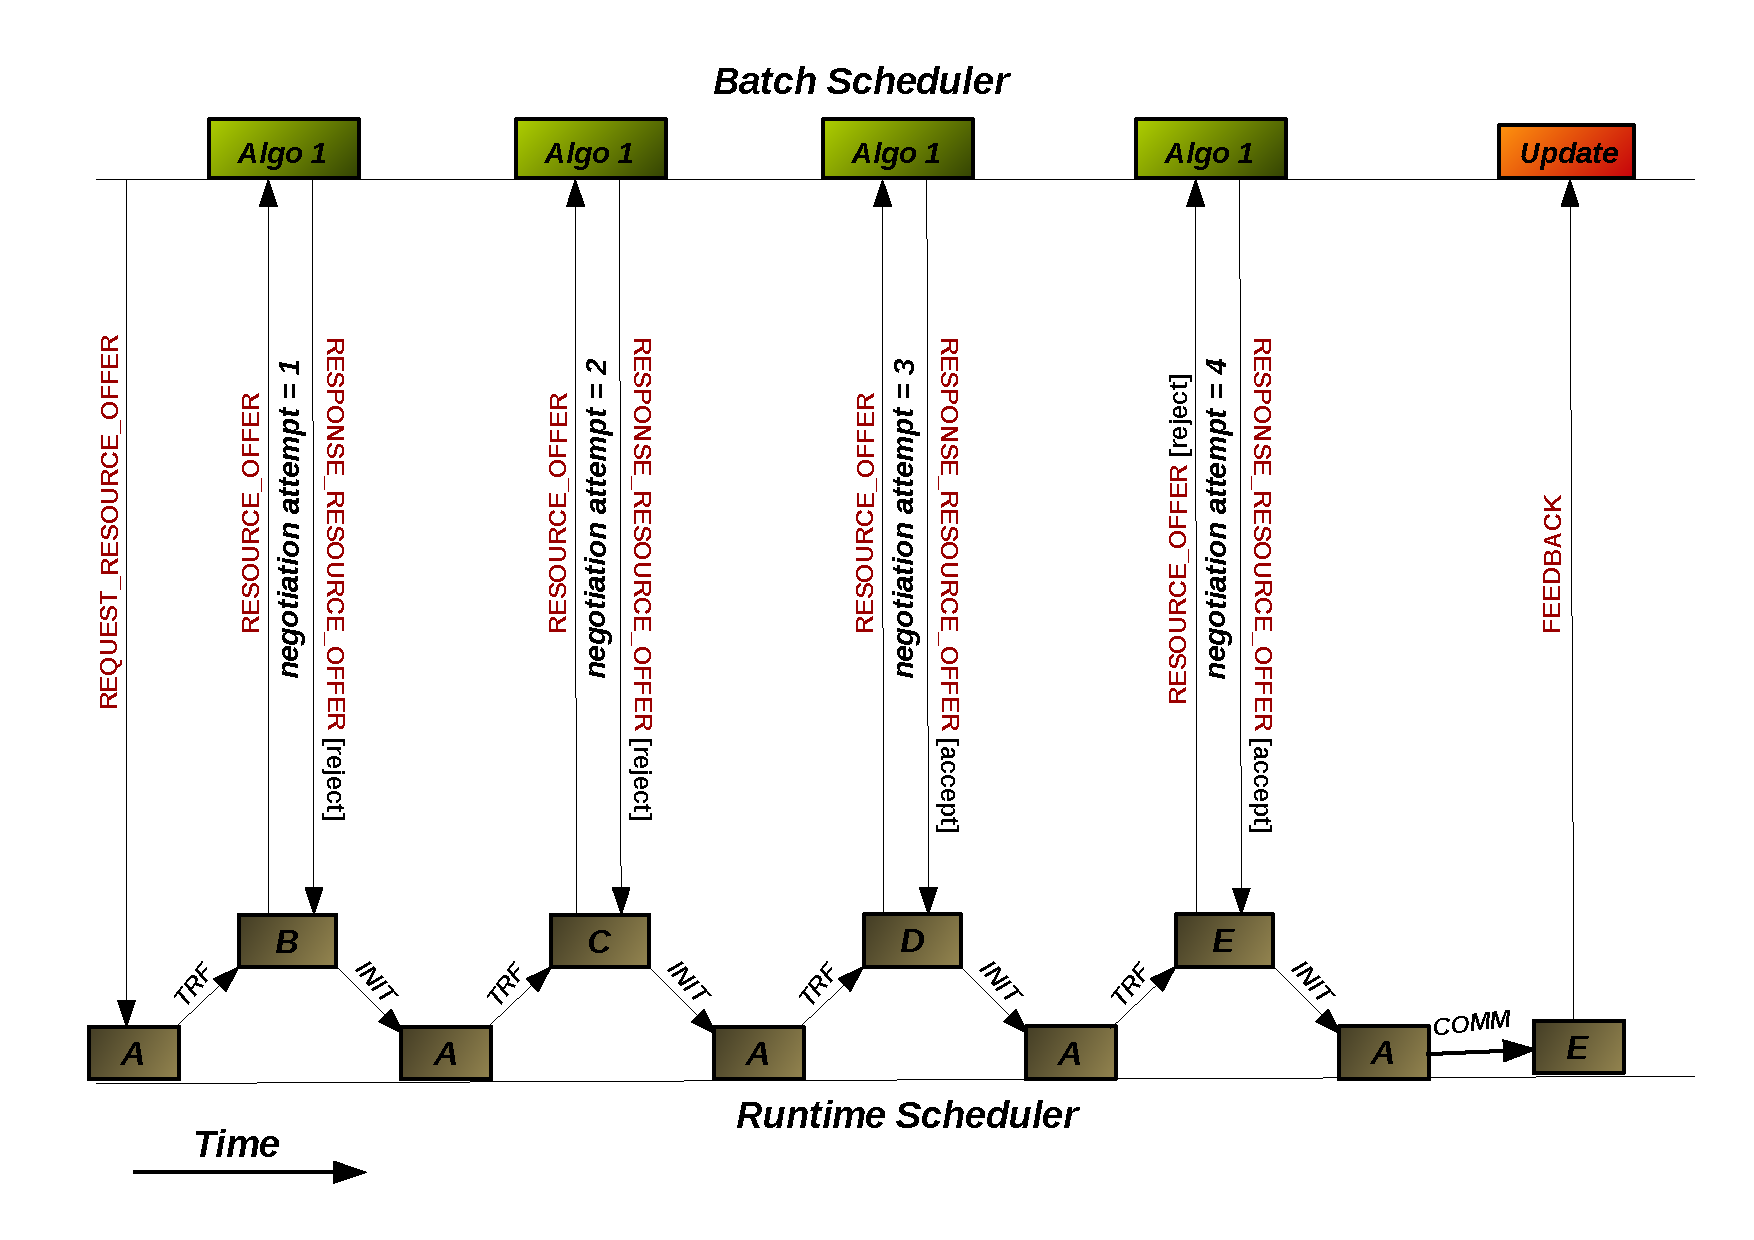
\includegraphics[width=1.2\textwidth, height=95mm]{./figures/negotiation.pdf}
\caption{Negotiation protocol}
\label{fig:2}
\end{figure}

\chapter{Implementation}\label{chapter:implementation}
\section{Plugin}
iBSched is implemented as an extension to SLURM in the form of a scheduler plugin. A Slurm plugin is a dynamically linked code object which is loaded explicitly at run time by the Slurm libraries. A plugin provides a customized implementation of a well-defined API connected to tasks such as authentication, interconnect fabric, and task scheduling. There are several other existing scheduler plugins of SLURM such as: the default(FCFS) plugin, Backfill, wiki and wiki2(Interfaces to external schedulers) etc. A related plugin that is of importance to scheduling is the priority plugin because the job queue is first constructed and then sorted based on priorities before the scheduling algorithm runs through it. Slurm provides a basic priroity plugin and a multifactor priority plugin. The basic version provides a standard FIFO based job priority whereas the multifactor version provides priorities to job based on several factors such as age, fair-share, job size(also considers the job duration to calculate a weight factor for job size relative to time), partition, quality of service etc. The multifactor priority plugin has been refactored for this work to be better suitable for our implementation. Specifically, the multifactor priority plugin now assigns priority to jobs based on age and size(relative to time). As its default behavior it periodically re-calculates the priorities of the jobs.\\ \\
%%%%%
For the current scope of the work, iRTSched has been implemented as an independent binary that talks to iBSched via the negotiation protocol. The purpose of this independent binary is to fake an actual runtime scheduler by simulating the runtime states of the system in time by employing the runtime scheduling algorithm and also negotiating with iBSched. In reality, a full-fledged runtime scheduler will be managing the resources in the invasic partition, will launch the jobs and perform dynamic resource management. In order to evaluate the negotiation-based separation of batch and runtime scheduling system, a simulation of the same would be very useful and sufficient for our objectives. 
\section{Data Structures}
This section will enumerate some of the important data structures that are a part of the implementation.\\ \\
\lstset{breaklines=true}
\textbf{Job Mappings}\\
Below is enum that represents the possible characterstics of a job. This hint can be supplied at job submission time or can be inferred during runtime and profiling the application performance. By default it will be considered as NONE.
\begin{lstlisting}[mathescape]
enum job_hint {
        COMP_BOUND,
        MEMORY_BOUND,
        IO_BOUND,
	NONE
};
\end{lstlisting}
Below is an enum that represents the type of a job. This needs to be specified at submission time by the user. By default it will be considered as rigid.
\begin{lstlisting}[mathescape]
enum job_type {
        RIGID,
        MOLDABLE,
        EVOLVING,
        MALLEABLE
};
\end{lstlisting}
Below structure represents the node count constraint that is used by the batch scheduler during the negotiations with runtime scheduler. At the submission time max will be set to the job's max nodes and min will be set to a value of max nodes - step\_size where step\_size is calculated from the formula given in x.x. This step will be repeated when a new transaction starts.
\begin{lstlisting}[mathescape]
typedef struct qos_rsrc {   
        uint32_t min;
        uint32_t max;
} qos_rsrc_t;
\end{lstlisting}
%%%%%%%%
Below structure represents the details of a job necessary for its launch. This is packed within the following structure and it gets forwarded to the runtime scheduler.
\begin{lstlisting}[mathescape]
struct forward_job_details {
        qos_rsrc_t node_count;          /* Job resource requirements */
        uint16_t cpus_per_task;         /* number of processors required for
                                         * each task */
        uint8_t hint;                   /* Job characteristic: IO / Compute / Memory bound */
        uint8_t job_type;                       /* Type of job: Static or Dynamic */
        /* Ideally this structure should further contain all the necessary details required for launching this job. For the purpose of this thesis, we are only doing a simulation without running jobs, hence other details in this structure are not important */
};
\end{lstlisting}
%%%%%%%
The below structure makes up a single entry in the Map that is constructed by batch scheduler. A list of such entries make up the mapping of jobs to offer which is sent to the runtime scheduler. In addition to the details of the job as mentioned for the previous structure, this structure include details such as the bitmap of nodes allocated, priority, job id, min / max nodes etc.
\begin{lstlisting}[mathescape]
struct forward_job_record {
        struct forward_job_details *details;    /* job details */
        uint32_t job_id;                /* job ID */
        uint32_t magic;                 /* magic cookie for data integrity */
        char *name;                     /* name of the job */
        bitstr_t *node_bitmap;          /* bitmap of nodes allocated to job */
        uint32_t node_cnt;              /* Current node count assigned */
        uint32_t min_nodes;
        uint32_t max_nodes;
        uint32_t priority;              /* relative priority of the job,
                                         * zero == held (don't initiate) */
        time_t start_time;              /* Expected or Actual start time */
        uint32_t time_limit;            /* time_limit minutes or INFINITE,
                                         * NO_VAL implies partition max_time */
        uint32_t time_min;              /* minimum time_limit minutes or
                                         * INFINITE,
                                         * zero implies same as time_limit */
};
\end{lstlisting}
%%%%%%%
Below structure represents the message used by batch scheduler to request for a resource offer. It contains a value field used for the purpose of protocol communication followed by the most important field which is the Map.
\begin{lstlisting}[mathescape]
typedef struct request_resource_offer_msg {
        uint16_t value; /* info */
        List jobs2map; /* This is the list of jobs waiting to be dispatched. And communicates the current requirements to rt scheduler which 
                          can then try to suitably construct a resource offer to satisfy the requirements as best as possible */
} request_resource_offer_msg_t;
\end{lstlisting}
%%%%%%%%
Below structure represents the response to a resource offer sent by the batch scheduler. It resembles very closely to the previous message but has in addition the error code and the error msg fields. These fields which identify the error are important for batch scheduler to convey its response to the runtime scheduler for the offer it sent.
\begin{lstlisting}[mathescape]
typedef struct resource_offer_resp_msg {
        uint16_t value;         /* info */
        List map_jobs2offer;    /* Jobs mapped to the given offer. This depends on whether the batch scheduler accepted / rejected / countered
                                 the resource offer it received */
        uint32_t error_code;    /* error code on failure */
        char   * error_msg;     /* error message on failure */
} resource_offer_resp_msg_t;
\end{lstlisting}
%%%%%%%
\textbf{Resource Offers}\\
Below structure represents the reservation for a job which can begin immediately or in the future. This depends on the response from the runtime scheduler.
\begin{lstlisting}[mathescape]
typedef struct job_resv {
        time_t end_time;        /* end time of reservation              */
        uint8_t full_nodes;        /* when reservation uses full nodes or not */
        uint32_t job_id;        /* job ID */
        bitstr_t *node_bitmap;  /* bitmap of reserved nodes             */
        uint32_t node_cnt;      /* count of nodes required              */
        time_t start_time;      /* start time of reservation            */
} job_resv_t;
\end{lstlisting}
Below structure represents the message format for resource offer message sent by runtime scheduler. It contains a list of reservations for each of the jobs that were sent by batch scheduler in its mapping. It contains the set of residual or free nodes available.
\begin{lstlisting}[mathescape]
typedef struct resource_offer_msg {
        uint16_t value;      /* info */
        uint8_t negotiation; /* if negotiation is ongoing then this value is 1 else it becomes 0 to indicate ischeduler that previous negotiat
                                ion is over */
        List resource_offer;   /* List of node space records */
        List resv_jobs;        /* List of jobs with actual reservations. Can also include jobs with virtual reservations that are those with
                                  future start / service times */
        uint32_t error_code;    /* error code on failure */
        char   * error_msg;     /* error message on failure */
} resource_offer_msg_t;
\end{lstlisting}
%%%%%%%%%%
\textbf{Feedback Reports}\\
Below structures represent the format of a feedback report and a list of reports respectively. For the scope of this current work, the feedback does not send back any performance model of the running / completed application or any kind of job characteristic and energy consumption. It sends across basic details about the status of running / completed jobs.
\begin{lstlisting}[mathescape]
typedef struct job_status {
        uint32_t job_id;
        time_t run_time;
        time_t end_time;
        uint32_t node_cnt;
        bitstr_t *node_bitmap;
        uint32_t job_state;
} job_status_t;

typedef struct status_report_msg {
        List status_reports;
} status_report_msg_t;
\end{lstlisting}
%%%%%%%%%%%
\textbf{Running Job Record}\\
The below structure is very important as the runtime scheduler uses this as the job record for each of the running jobs. Since the scope of this work is simulation, We do not include many other details of a job that would be necessary for its launch, logging etc. Dependency of a forwarded job onto a running malleable job is saved in the variables depend\_job\_id and depend\_job\_prio of a running job record. This dependency information is used by the PDBES algorithm.
\begin{lstlisting}[mathescape]
struct run_job_record {
        uint32_t job_id;
        bitstr_t *node_bitmap;
        time_t start_time;
        uint32_t priority;
        uint32_t time_limit;
        uint8_t hint;
        uint8_t job_type;
        time_t end_time;
        time_t orig_end_time;
        uint32_t job_state;
        uint32_t orig_node_cnt;
        uint32_t node_cnt;
        uint32_t last_node_cnts[2];
        bitstr_t *next_node_bitmap;
        uint32_t next_node_cnt;
        uint32_t depend_job_id;
        uint32_t depend_job_prio;
        uint32_t save_depend_job_id;
        uint32_t save_depend_job_prio;
        uint32_t min_nodes;
        uint32_t max_nodes;
        uint8_t adapt;  /* 0 - No change, 1 - Expand, 2 - Shrink */
        uint8_t transformed;
        time_t exp_end_time;
};
\end{lstlisting}
%%%%%%%
\textbf{Node Space Map}\\
Below is an existing structure used by SLURM for its backfilling algorithm. This is used to form a chain of records chronologically ordered in time that represent the set of available nodes in those timeslots. The backfill algorithm uses this structure to prepare the view of resources in time and resembles a two dimensional space of nodes and time. This is used in order to compute when and where a job can start by looking at the reservations that higher priority jobs already have and these must be respected by lower priority jobs in case they can start now.
\begin{lstlisting}[mathescape]
typedef struct node_space_map {
        time_t begin_time;
        time_t end_time;
        bitstr_t *avail_bitmap;
        int next;       /* next record, by time, zero termination */
} node_space_map_t;
\end{lstlisting}
%%%%%%%%
\section{Important APIs}
\begin{lstlisting}[mathescape,frame=single]
extern List schedule_invasic_jobs(resource_offer_msg_t *, List, uint16_t *, uint32_t *);
\end{lstlisting}
This routine is responsible for creating a map of jobs to the available offer. It will fill the offer that has been passed as a an argument to it with the list of invasive jobs that have been selected according to its algorithm. Jobs in this list would be mapped to some number of nodes that satisfy the job constraints. Those jobs which could not be mapped will have their constraints relaxed and just forwarded along with other jobs. Also, The batch scheduler has a limit on the number of jobs that can be forwarded but have not been mapped to any resources as it did not satisfy its constraints. This is the reservation depth similar to what is used in backfill algorithms. Once the limit has been reached the scheduling algorithm will then just scan the rest of the invasive job queue to look for jobs that can fit the remaining available nodes in the offer.\\ 
\begin{lstlisting}[mathescape,frame=single]
extern uint32_t adjustQoS_node_count(struct job_record *);
\end{lstlisting}
This routine relaxes the node count constraint of a job. The original constraints are min and max nodes supplied at the job submission time. Negotiation begins by setting a node count constraint(node\_count.min, node\_count.max) within this window of min and max. With more negotiation attempts in a single transaction, the constraints would keep getting relaxed and node\_count.min would approach the original min value.\\
\begin{lstlisting}[mathescape,frame=single]
extern void resetQoS_node_counts();
\end{lstlisting}
This routine is called before the start of a new set of negotiations. It will reset the node count constraint for every job in the queue to their original values.\\
\begin{lstlisting}[mathescape,frame=single]
extern int _decision_logic(List, int, uint32_t);
\end{lstlisting}
This routine is where the batch scheduler makes a final decision on whether the received resource offer form runtime scheduler is accepted / rejected. It does so by checking through the mapping that has been constructed after the scheduling algorithm processed the offer. The mapping is supplied as the first argument to this function.\\
\begin{lstlisting}[mathescape,frame=single]
extern void *irm_agent(void *);
\end{lstlisting}
This is the routine that is associated with the main runtime scheduler thread. It gets called once the thread has been created. It basically runs an infinite control loop for the scheduler to initiate various operations such as processing the response for an offer from batch scheduler, performing a transformation of the runtime system state, waiting for a request for resource offer in a separate spawned thread, sending back an offer to batch scheduler, terminating the scheduler etc.\\
\begin{lstlisting}[mathescape,frame=single]
extern int process_resource_offer(resource_offer_msg_t *, uint16_t *, int *, List *, List);
\end{lstlisting}
This routine initiates the processing of a resource offer, calls the appropriate scheduling algorithm.\\
\begin{lstlisting}[mathescape,frame=single]
extern int _request_resource_offer(slurm_fd_t);  /* Wrapper for request_resource_offer to construct the list of job requirements to be sent */
\end{lstlisting}
This routine sends a request for resource offer to the runtime scheduler. It does so by constructing a list of job requests to be forwarded.\\
%%%%%%%%%%%%%
\begin{lstlisting}[mathescape,frame=single]
extern int process_rsrc_offer_resp(resource_offer_resp_msg_t *, int, resource_offer_msg_t **);
\end{lstlisting}
This routine is responsible for processing the mapping received from the batch scheduler and invoking the appropriate runtime scheduling algorithm. If the response from batch scheduler was accept for its previous offer, then it will recreate the transformation of the previous attempt else it will create a new transformation. It will run the algorithm to satisfy as many jobs forwarded as possible by using the PDBES algorithm and then determine whether it will accept / reject this mapping. If it does not accept then it will send a new offer created as a result of this new transformation.\\
\begin{lstlisting}[mathescape,frame=single]
extern int create_resource_offer(int, List, uint16_t, resource_offer_msg_t **);
\end{lstlisting}
This routine is called from within the "process\_rsrc\_offer\_resp" routine to initiate the scheduling algorithm to run through the mapping. It is also called in the "irm\_agent" routine in situations when a request for a resource offer is received. Or, a new offer needs to be generated by the runtime scheduler since some running applications have shrunk to create a gap in the resources that can be utilized to serve some new batch jobs.\\
\begin{lstlisting}[mathescape,frame=single]
static int 
_schedule(int attempts, List job_queue,
                uint16_t *recv_err_code, resource_offer_msg_t **rsrc_offer_msg);
\end{lstlisting}
This is the runtime scheduling algorithm whose steps have been described in the form of a pseudo code x.x.x. It will use the PDBES algorithm to scan through the mapping and provide start times for each of them.\\
\begin{lstlisting}[mathescape,frame=single]
extern bitstr_t * _try_transf(bool);
\end{lstlisting}
This routine performs a runtime transformation of the system state by performing expand / shrink of the running malleable jobs considering their performance and scalability. In case the result of this transformation are some free resources, then those will be sent up to batch scheduler as a new resoruce offer. The boolean argument passed here represents the negotiation flag. If it is true then it means we have received a request for an offer and must perform a partial transformation by doing only the shrink operations to create a gap in the resources. If it is false then it means that we must do the full transformation as no offer is being sent out.\\
\begin{lstlisting}[mathescape,frame=single]
extern int _commit_state(bool);
\end{lstlisting}
This routine will commit the forwarded jobs(with immediate start time) to the running jobs list. It will also change the node bitmaps of running jobs to their new node bitmaps if they have been subjected to some sort of transformation during the phase of runtime scheduling algorithm. In alignment with the new node counts for many of the running malleable jobs, there expected end times will also be updated based on whatever performance model is know until this point.\\
\begin{lstlisting}[mathescape,frame=single]
extern bool _get_delta(uint32_t *, time_t, time_t);
\end{lstlisting}
This routine will compute the next time slice for which the runtime scheduler will sleep. This could be a fixed time interval for periodic wake ups of the runtime scheduler or it can wake up earlier if there was some job that is expected to complete within this time interval.
\begin{lstlisting}[mathescape,frame=single]
extern void _initialize_state(void);
\end{lstlisting}
This routine resets the state of the system back to the point before the start of the negotiation. During the negotiation process, a lot of the details in the running job records would be temporarily updated to account for negotiations and the associated expand / shrink operations. With every negotiation attempt within a transaction, the state will have to be reset before the runtime scheduler can run its algorithm again.\\
\begin{lstlisting}[mathescape,frame=single]
extern int _decision_logic(resource_offer_msg_t *, List, int, bool);
\end{lstlisting}
The runtime scheduler decides whether to accept / reject the mapping received from batch scheduler by calling this routine. This routine checks through the mapping to see how many jobs can be started immediately and based on how well it is suitable for its metrics a decision will be taken.
%%%%%%%%%%%%%
\section{State Machine Diagrams}
Following pages give the state machines diagrams of both the batch and the runtime scheduler. These diagrams illustrate their implementation and the general flow of their working highlighting the important details. Many of the error handling or subordinate threads related to feedback, urgent job handling, signal handling for termination etc. have not been shown here due to space constraints. The diagrams in both the pages represent the main control thread for both the batch and runtime scheduler. This control thread is responsible to spawn other subordinate threads, drive the control loop responsible for doing / initiating all the work such as receiving processing and sending protocol messages.\\ \\
%%%%%%%%
\begin{figure}[!htbp]
\hspace*{0.1in}
\centering
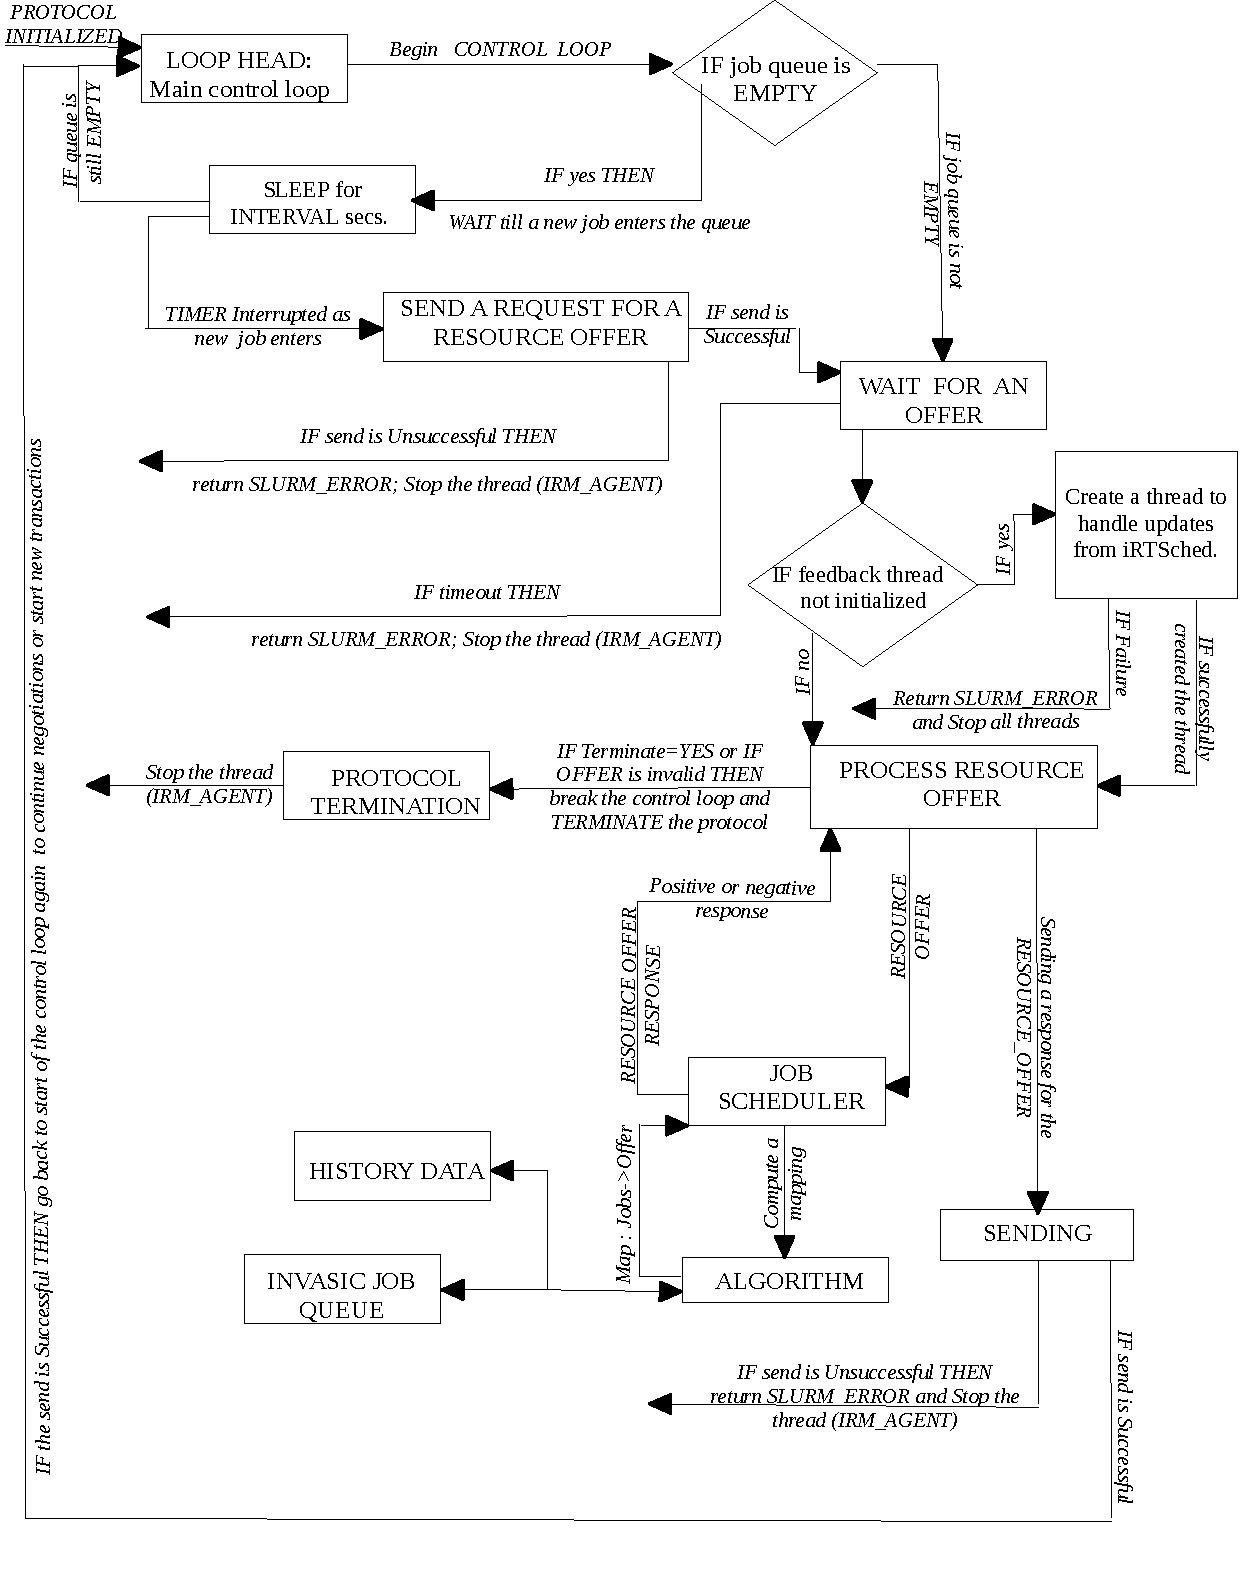
\includegraphics[width=1.0\textwidth, height=195mm]{./figures/iBSched.pdf}
%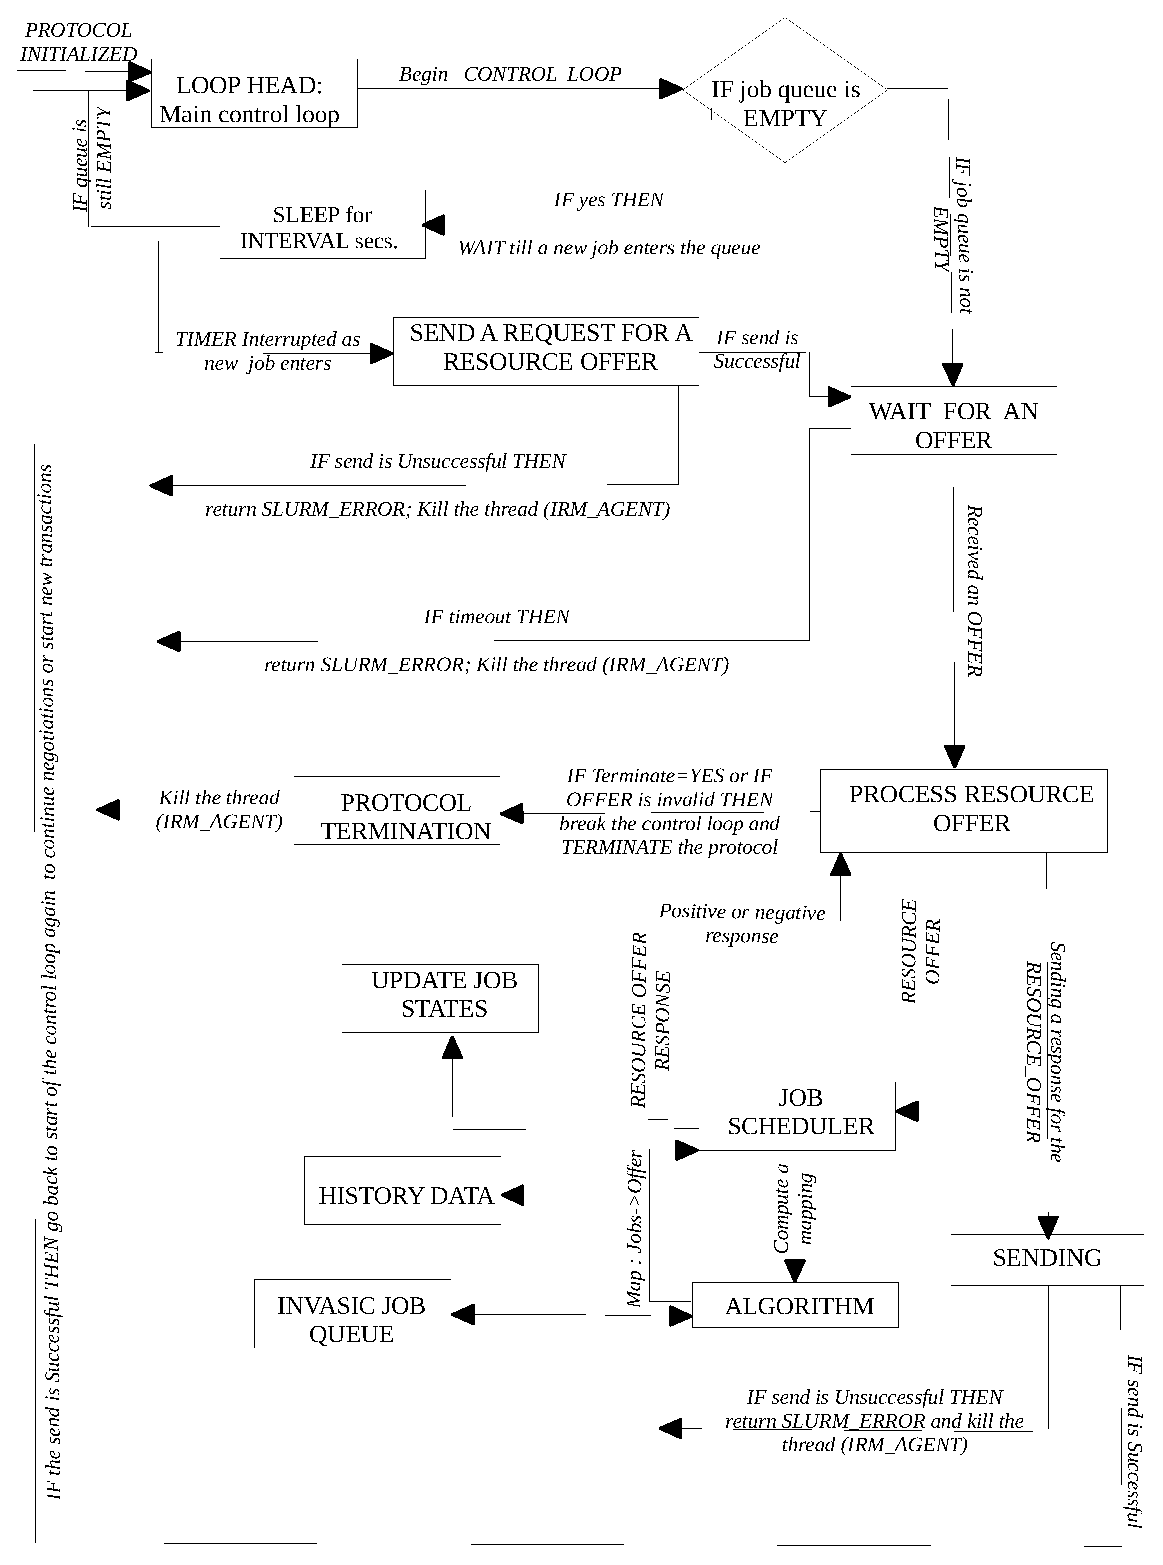
\includegraphics[width=1.0\textwidth, height=180mm]{./figures/Negotiation.eps}
\caption{iBSched}
\label{fig:Neg}
\end{figure}
\noindent
iBSched is a SLURM plugin, hence it is dynamically loaded by the SLURM controller(slurmctld) due to which a plugin initialization happens for iBSched during which a main plugin thread is created. This plugin thread is then responsible to create the main control thread for iBSched. The plugin thread is responsible for starting and shutting down this plugin(in case slurmctld sends a shutdown signal) and other threads it spawned. The main control thread is responsible for shutting down all the slave threads it had spawned. iRTSched also has multithreaded design exactly similat to iBSched except that it is an independent binary and is launched independently but not by any SLURM application.
%\begin{figure}[!htbp]
%\hspace*{0.1in}
%\centering
%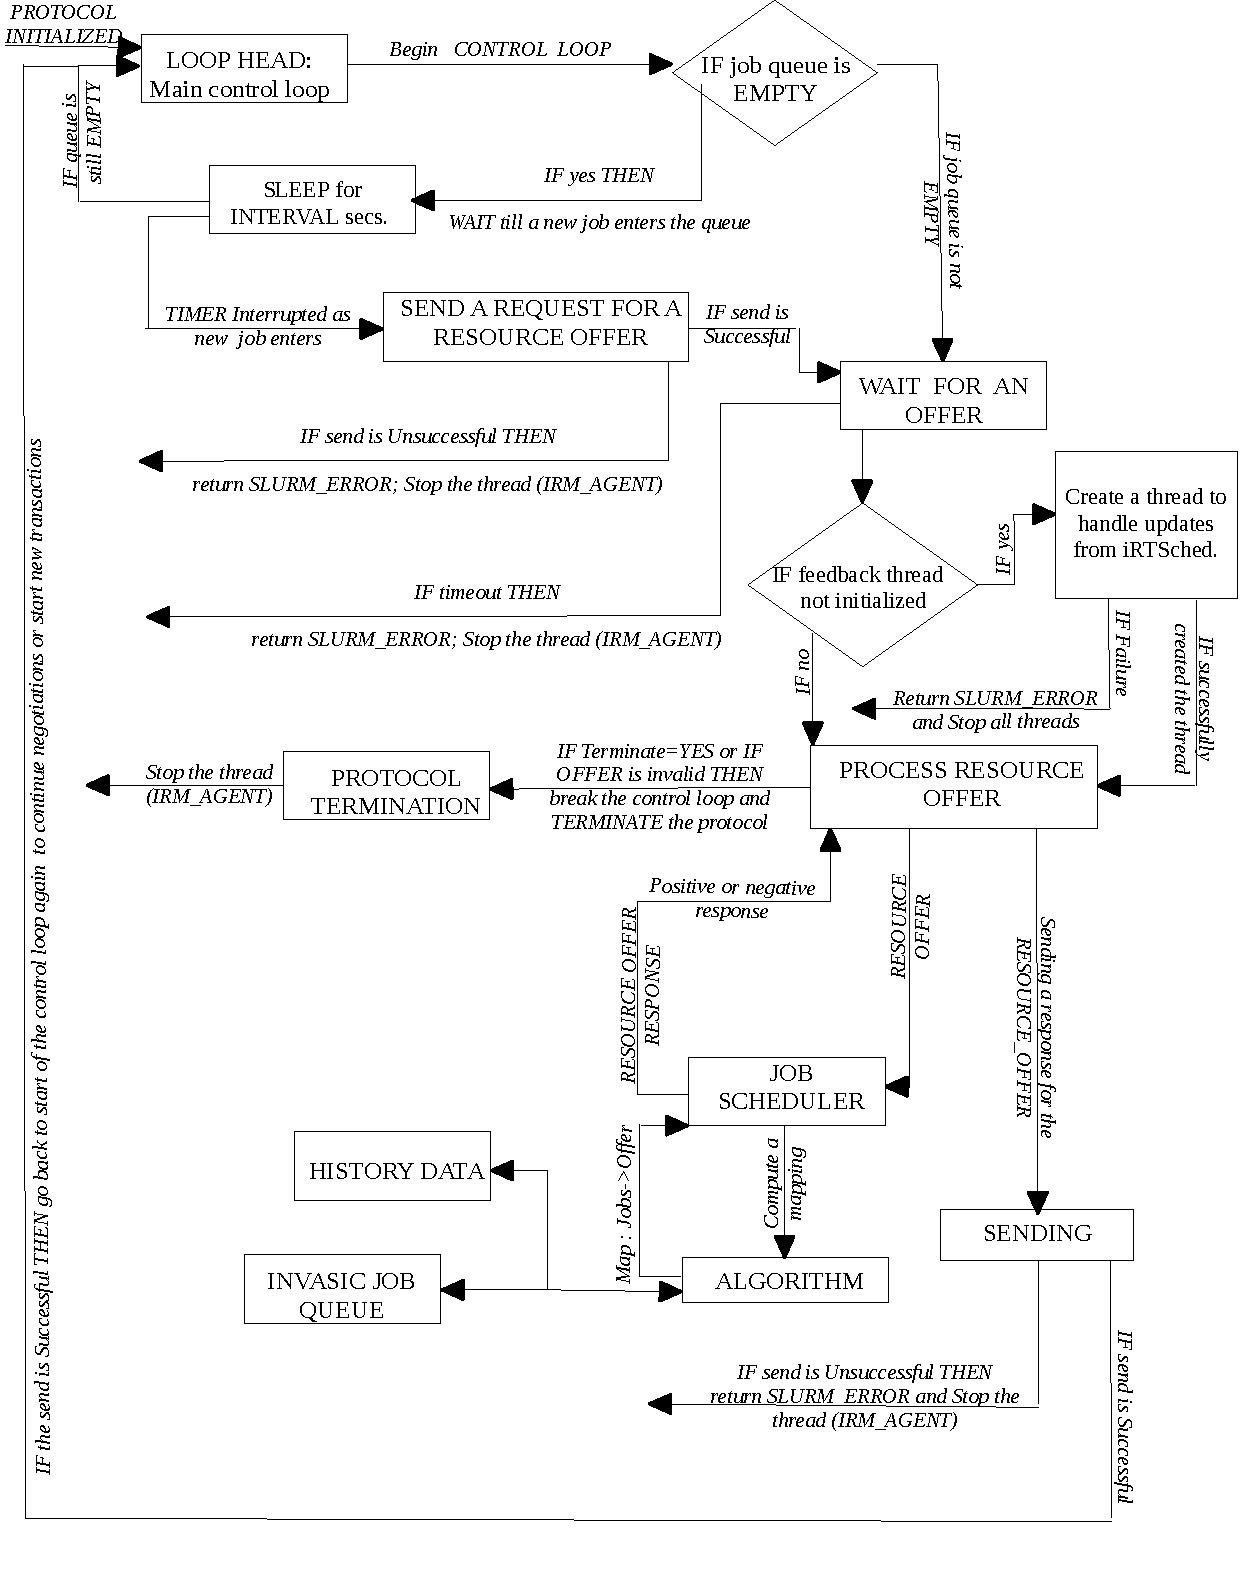
\includegraphics[width=1.0\textwidth, height=195mm]{./figures/iBSched.pdf}
%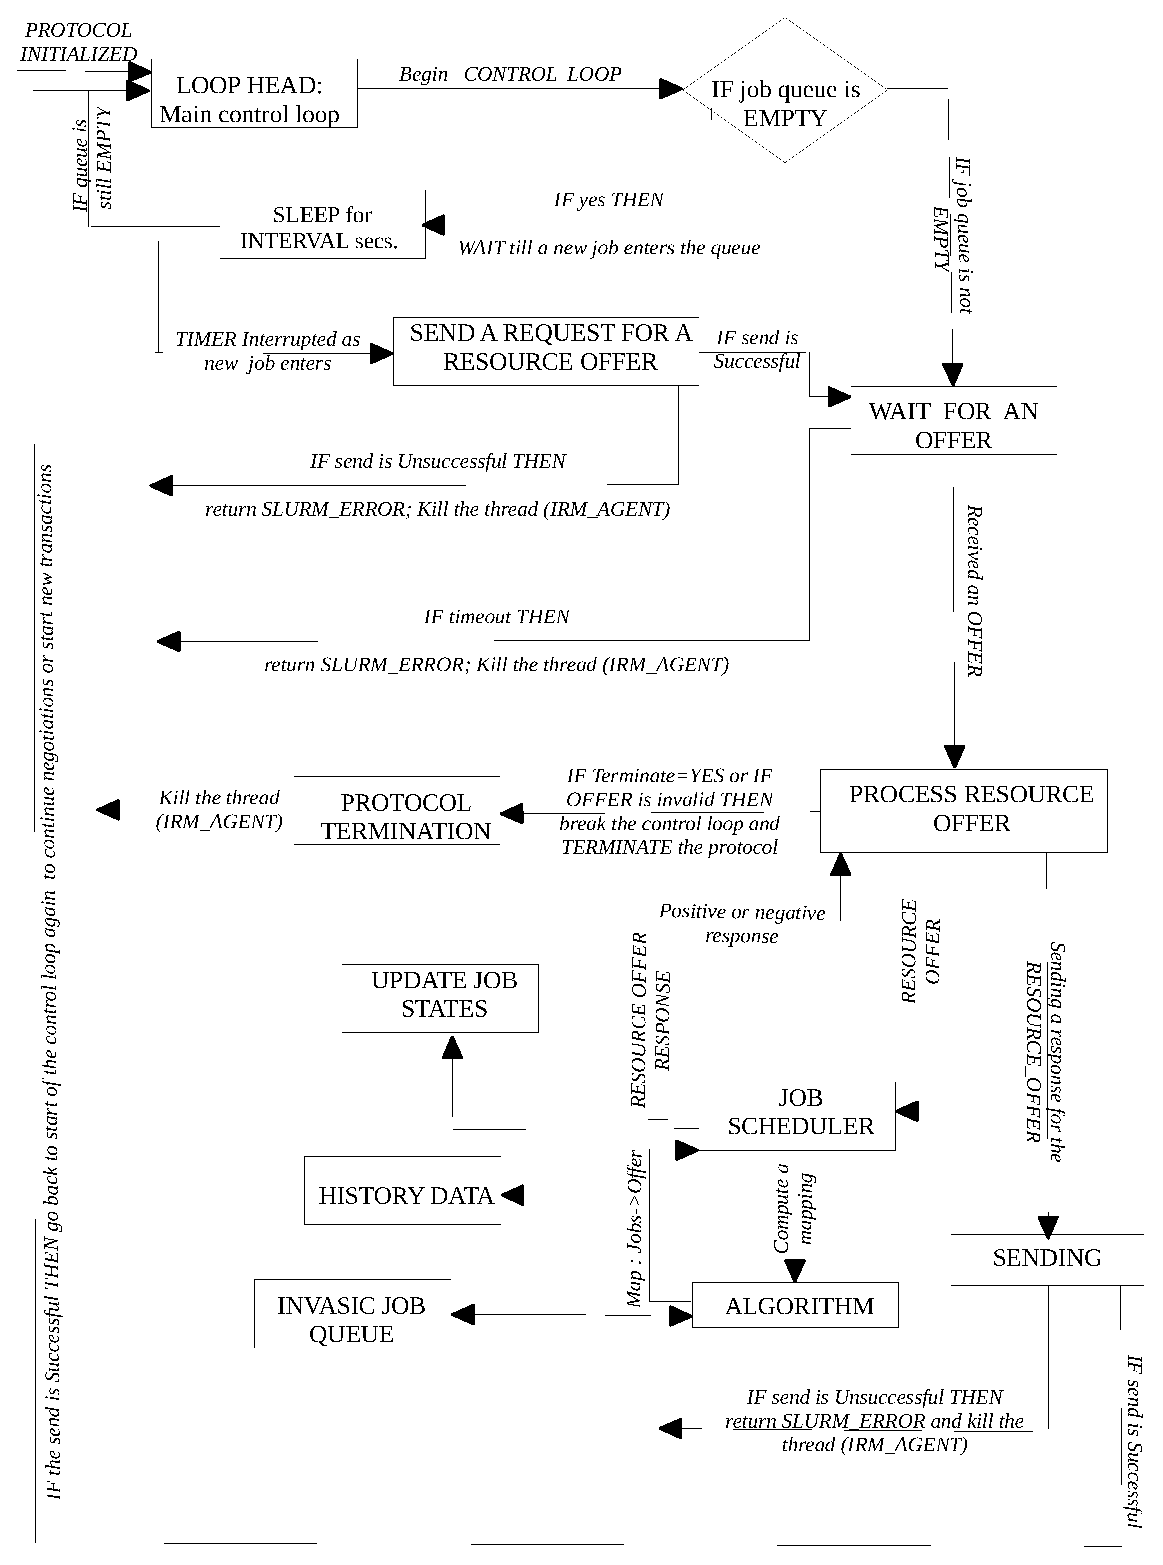
\includegraphics[width=1.0\textwidth, height=180mm]{./figures/Negotiation.eps}
%\caption{iBSched}
%\label{fig:Neg}
%\end{figure}
\begin{figure}[!htbp]
\centering
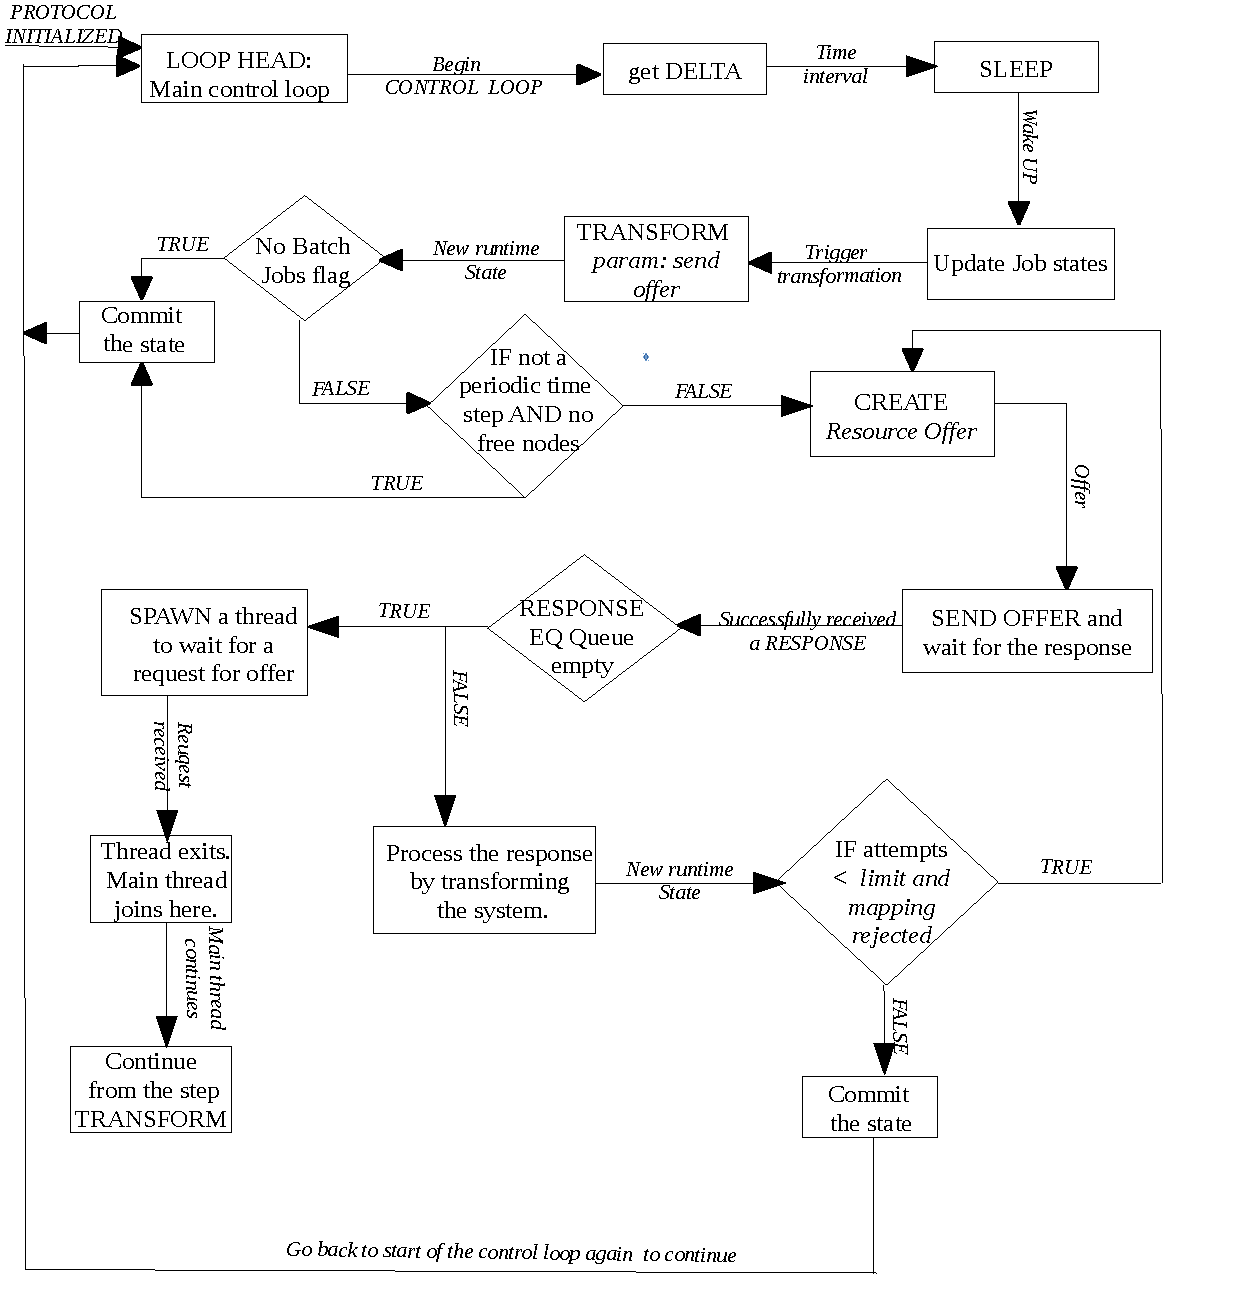
\includegraphics[width=1.0\textwidth, height=160mm]{./figures/iRTSched.pdf}
%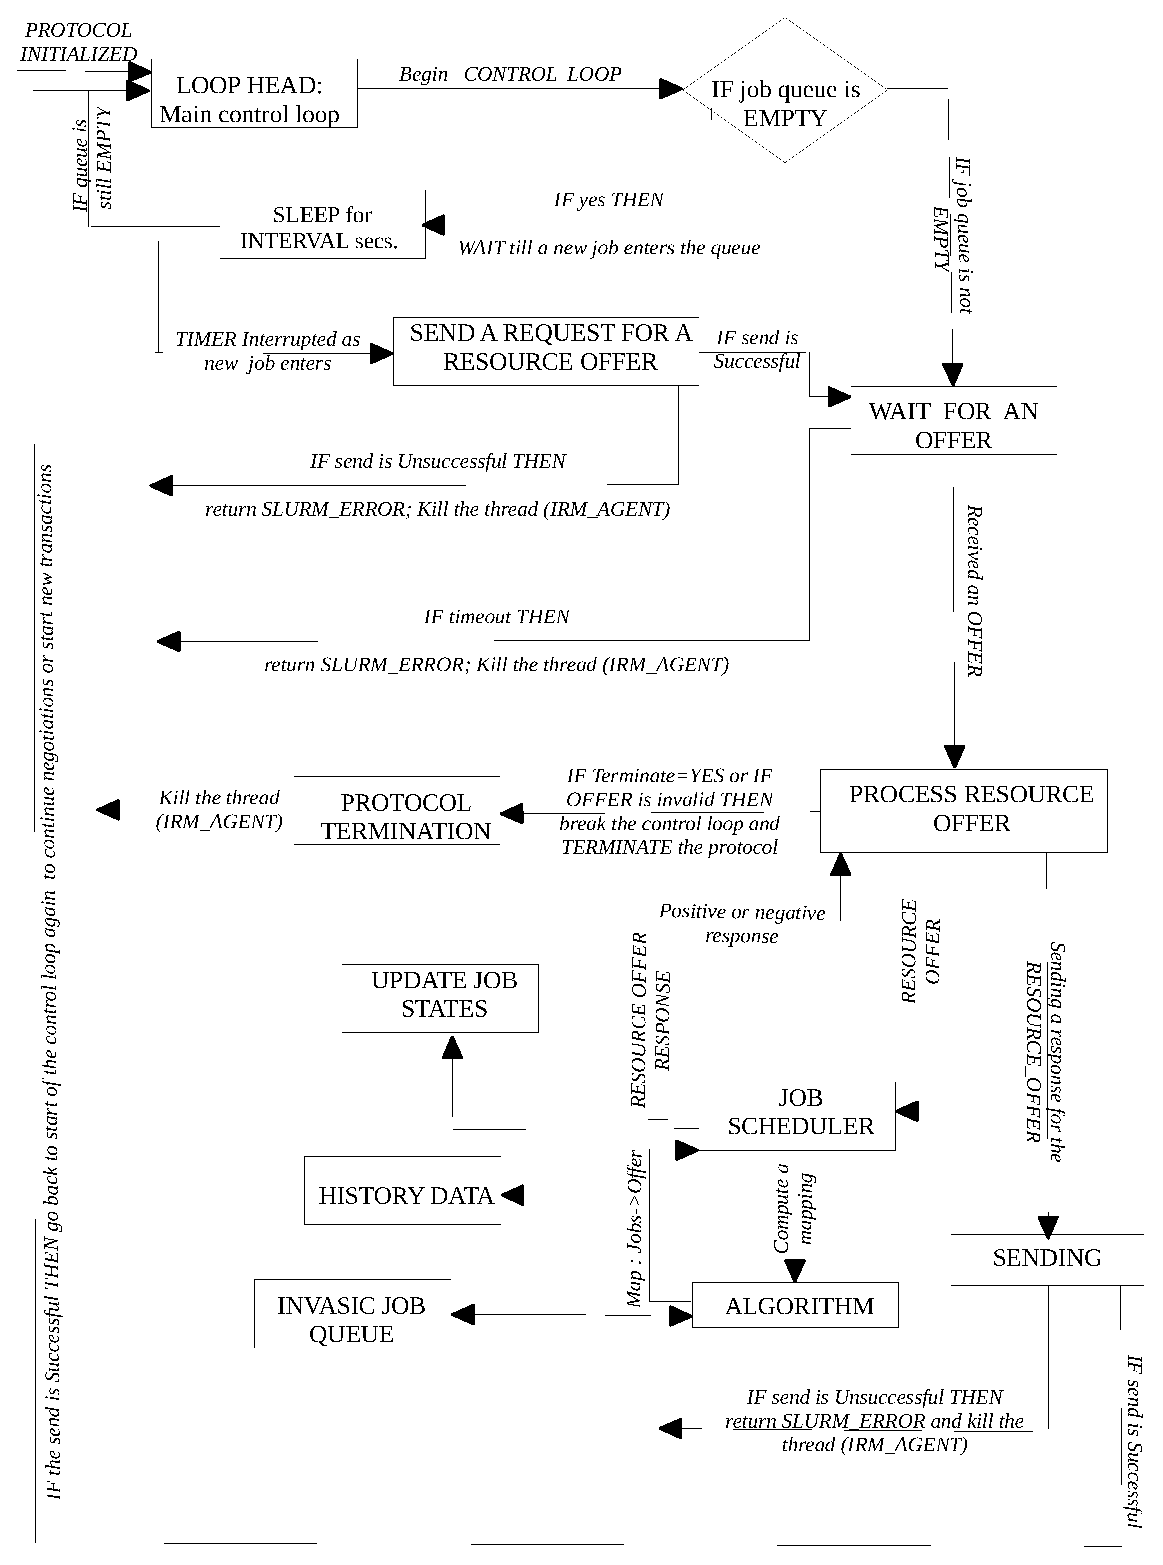
\includegraphics[width=1.0\textwidth, height=180mm]{./figures/Negotiation.eps}
\caption{iRTSched}
\label{fig:Neg1}
\end{figure}

\chapter{Evaluation}\label{chapter:evaluation}
May be a page illustrating a scenario of negotiation with 2d node space map diagrams will be good.
\section{Method of Evaluation}
\subsection{Emulation of Workload}
\subsection{Real Invasic Applications}
\section{Setup}
\section{Experiments and Results}
\section{Performance and Graphs}

\chapter{Conclusion and Future Work}\label{chapter:conclusion and future}
The objective of this Master Thesis was to explore the idea of separating the concerns of batch and runtime scheduling with the help of a negotiation protocol to provide a dynamic and flexible scheduling strategy for adaptive applications. A prototype realizing this idea has been successfully designed and implemented with scheduling algorithms for both batch and runtime scheduler respectively. The runtime scheduling algorithm is based on the recently proposed \textbf{\textit{DBES}} algorithm that has been adapted for being suitable to negotiation. The batch scheduler uses a simple but effective algorithm to compute an approximation of the best-fit selection of jobs to a given resource offer through one or more negotiations. This approach of splitting up the batch and runtime concerns by using a negotiation protocol was named as \textbf{\textit{DN-DBES}} algorithm in this thesis. The proposed objectives in the thesis were successfully achieved with satisfactory performance of the simulations for malleable-rigid and moldable-rigid workloads. Following are a few final observations:
\begin{itemize}
\item The expected end times of the running malleable jobs are adjusted by the runtime scheduler only after the job has reached its first periodic runtime transformation step. This will most likely happen after a fixed interval of time or when a job terminates / completes earlier than this interval. In both the cases it is soon after the job has started.
\item This implies that some time in the early part of the job execution is accounted for using only the minimum number of nodes though the job may be running with more than minimum number of nodes. 
\item This was done to simulate what happens in a real system where continuous performance data collected is used for making expand or shrink decisions for an application. But on a real system, the same job may finishes sooner than the simulated system.
\item In a simulation, we create the runtime states of the system and change it with time. Hence, in a real system with exactly the same workloads as the once used in experiments with the same application having linear speedup curves should produce much faster completion times in the case of malleable-rigid workloads. This is similarly the case for moldable jobs in the moldable-rigid workload.
\item Batch and runtime scheduling algorithms run in O($n^{2}$) time complexity for the worst case scenario. A set of negotiations within a transaction does not change this either. Simulations show that it is consuming neglibile time for the experimented workloads. Every transaction consumes not more than $1-2$ seconds in total.
\item These latencies will however be hidden in a real system. This is because the negotiations will happen before the actual transformation of the running jobs is done by the runtime scheduler at its periodic time step. Before this periodic time step, the computation of the transformation and the possibility of new batch jobs for the runtime scheduler are already completed.
\item These factors will again reduce the completion time in a real system compared to the simulation where the latencies are counted by the simulation clock.
\end{itemize}
\section{Future Work}
Below mentioned are some of the possible directions for future research work:
\begin{itemize}
\item Integrating the iRTSched from this prototype with the real iRTSched which is capable of managing resources along with providing the elastic execution model for applications. The full solution stack should then be tested with real workload containing real invasive applications.
\item Runtime performance modeling of the applications should be performed and the model should then be used to estimate the performance and scalability of the applications at different job sizes. This information should then be used for making expand or shrink decisions.
\item Batch scheduling algorithm currently uses an FCFS like algorithm with backfilling style approach in its final step to rescan the invasive job queue and update the job list. Many different algorithms can be used instead of this approach.
\item One such algorithm could be to look at a window of jobs in the batch queue and select the best combination using a knapsack algorithm or by mathematically modeling it in the form of an integer program and solving the same.
\item The negotiation protocol and the batch scheduling algorithm can be enhanced to communicate with multiple runtime schedulers. This can resemble a grid like infrastructure but for a supercomputer this may resemble the different partitions of the system.
\end{itemize}

% TODO: add more chapters here

\appendix{}

 % TODO: remove if glossary not needed
%\glsaddall{} % add all defined terms to glossary, even if not referenced in text
%\printglossaries{}

\microtypesetup{protrusion=false}
\microtypesetup{protrusion=true}
\printbibliography{}

\end{document}
